%
% PROJECT: <ETD> Electronic Thesis and Dissertation Initiative
%   TITLE: LaTeX report template for ETDs in LaTeX
%  AUTHOR: Neill Kipp, nkipp@vt.edu
%     URL: http://etd.vt.edu/latex/
% SAVE AS: etd.tex
% REVISED: September 6, 1997 [GMc 8/30/10]
% 

% Instructions: Remove the data from this document and replace it with your own,
% keeping the style and formatting information intact.  More instructions
% appear on the Web site listed above.

\documentclass[12pt,english]{report}

\makeatletter
\newif\if@restonecol

\let\algorithm\relax
\let\endalgorithm\relax
%\usepackage[tight,footnotesize]{subfigure}
\usepackage{subfigure}
\usepackage {paralist}
\usepackage{comment}
\usepackage{array}
\usepackage{amsmath}
\usepackage{graphicx}
\usepackage{amssymb}
\usepackage{cite}
\usepackage{url}
\usepackage[ruled]{algorithm2e}
\usepackage{babel}
\usepackage{listings}
\usepackage[pdftex, breaklinks,colorlinks=false,pdfborder={0 0 0}]{hyperref}
\usepackage[all]{hypcap}
\makeatother
\makeatletter
\providecommand{\tabularnewline}{\\}


\newtheorem{clm}{Claim}
\newtheorem{proof}{Proof}
\newtheorem{mydef}{Definition}


\makeatletter

%%%%%%%%%%%%%%%%%%%%%%%%%%%%%% LyX specific LaTeX commands.
\pdfpageheight\paperheight
\pdfpagewidth\paperwidth

%% Because html converters don't know tabularnewline
\providecommand{\tabularnewline}{\\}
%% A simple dot to overcome graphicx limitations
\newcommand{\lyxdot}{.}


%%%%%%%%%%%%%%%%%%%%%%%%%%%%%% User specified LaTeX commands.



\makeatother



\setlength{\textwidth}{6.5in}
\setlength{\textheight}{8.5in}
\setlength{\evensidemargin}{0in}
\setlength{\oddsidemargin}{0in}
\setlength{\topmargin}{0in}

\setlength{\parindent}{0pt}
\setlength{\parskip}{0.1in}

% Uncomment for double-spaced document.
% \renewcommand{\baselinestretch}{2}

% \usepackage{epsf}

\begin{document}

\thispagestyle{empty}
\pagenumbering{roman}
\begin{center}

% TITLE
{\Large 
Real-Time Software Transactional Memory: Contention Managers, Time Bounds, and Implementations
}

\vfill

Mohammed El-Shambakey

\vfill

Preliminary Examination Proposal submitted to the Faculty of the \\
Virginia Polytechnic Institute and State University \\
in partial fulfilment of the requirements for the degree of

\vfill

Doctor of Philosophy \\
in \\
Computer Engineering

\vfill

Binoy Ravindran, Chair \\
Robert P. Broadwater \\
Cameron D. Patterson \\
Mohamed Rizk Mohamed. Rizk\\
Anil Kumar S. Vullikanti

\vfill

May 30, 2012\\
Blacksburg, Virginia

\vfill

Keywords: Software Transactional Memory, Embedded Systems, Contention Managers
\\
Copyright 2012, Mohammed El-Shambakey

\end{center}

\pagebreak

\thispagestyle{empty}
\begin{center}

{\large Real-Time Software Transactional Memory: Contention Managers, Time Bounds, and Implementations}

\vfill

Mohammed El-Shambakey

\vfill

(ABSTRACT)

\vfill

\end{center}

Lock-based concurrency control suffers from programmability, scalability, and composability  challenges. These challenges are exacerbated in emerging multicore architectures, on which improved software performance must be achieved by exposing greater concurrency.   Transactional memory (TM) is an alternative synchronization model for shared memory objects that promises to alleviate these difficulties. 

In this dissertation proposal, we consider software transactional memory (STM) for concurrency control in multicore real-time software, and present a suite of real-time STM contention managers for resolving transactional conflicts. The contention managers are called RCM, ECM, LCM, and PNF. RCM and ECM resolve conflicts using fixed and dynamic priorities of real-time tasks, respectively, and are naturally intended to be used with the fixed priority (e.g., G-RMA) and dynamic priority (e.g., G-EDF) multicore real-time schedulers, respectively. LCM resolves conflicts based on task priorities as well as atomic section lengths, and can be used with G-EDF or G-RMA.
%SH-ST
 Transactions under ECM, RCM and LCM can retry due to non-shared objects with higher priority tasks. PNF avoids this problem.
%SH-END

We establish upper bounds on transactional retry costs and task response times under all the contention managers through schedulability analysis. Since ECM and RCM conserve the semantics of the underlying real-time scheduler, their maximum transactional retry cost is double the maximum atomic section length. This is improved in the the design of LCM, which achieves  shorter retry costs.  However, ECM, RCM, and LCM are affected by transitive retries when transactions access multiple objects. 
Transitive retry causes a transaction to abort and retry due to another non-conflicting transaction.  
PNF avoids transitive retry, and also optimizes processor usage by lowering the priority of retrying transactions, enabling other non-conflicting transactions to proceed. 

We also formally compare the proposed contention managers with lock-free synchronization. 
Our comparison reveals that, for most cases, ECM, RCM, G-EDF(G-RMA)/LCM achieve higher schedulability than lock-free synchronization only when the atomic section length does not exceed half of the lock-free retry loop length. Under PNF, atomic section length can equal length of retry loop.
%SH-ST
 With low contention, atomic section length under ECM can equal retry loop length while still achieving better schedulabiltiy. While in RCM, atomic section length can exceed retry loop length. By adjustment of LCM design parameters, atomic section length can be of twice length of retry loop under G-EDF/LCM. While under G-RMA/LCM, atomic section length can exceed length of retry loop.
 %SH-EDF

We implement the contention managers in the Rochester STM framework and conduct experimental studies using a multicore real-time Linux kernel. Our studies confirm that, the contention managers achieve orders of magnitude shorter retry costs than lock-free synchronization. Among the contention managers, PNF performs the best.

Building upon these results, we propose real-time contention managers that allow nested atomic sections -- an open problem -- for which STM is the only viable non-blocking synchronization solution. Optimizations of LCM and PNF to obtain improved retry costs and greater schedulability advantages are also proposed. 

\vfill

% GRANT INFORMATION

%\textbf{NEEDS TO BE WRITTEN}

\pagebreak

% Dedication and Acknowledgments are both optional
% \chapter*{Dedication}
% \chapter*{Acknowledgments}

\tableofcontents
\pagebreak

\listoffigures
\pagebreak

\listoftables
\pagebreak

\listofalgorithms
\pagebreak

\pagenumbering{arabic}
\pagestyle{myheadings}

\chapter{\label{ch:introduction}Introduction}
\markright{Mohammed El-Shambakey \hfill Chapter~\ref{ch:introduction}. Introduction \hfill}

Embedded systems sense physical processes and control their behavior, typically through feedback loops. Since physical processes are concurrent, computations that control them must also be concurrent, enabling them to process multiple streams of sensor input and control multiple actuators, all concurrently. Often, such computations need to concurrently read/write shared data objects. Typically, they must also process sensor input and react, satisfying application-level time constraints. 

The de facto standard for programming concurrency is the threads abstraction, and the de facto synchronization abstraction is locks. Lock-based concurrency control has significant programmability, scalability, and composability challenges~\cite{Herlihy:2006:AMP:1146381.1146382}. Coarse-grained locking (e.g., a single lock guarding a critical section) is simple to use, but permits no concurrency: the single lock forces concurrent threads to execute the critical section sequentially, in a one-at-a-time order. This is a significant limitation, especially with the emergence of multicore architectures, on which improved software performance must be achieved by exposing greater concurrency.  

With fine-grained locking, a single critical section is broken down into several critical sections -- e.g., each bucket of a hash table is guarded by a unique lock. Thus, threads that need to access different buckets can do so concurrently, permitting greater parallelism. However, this approach has low programmability: programmers must acquire only necessary and sufficient locks to obtain maximum concurrency without compromising safety, and must avoid deadlocks when acquiring multiple locks. Moreover, locks can lead to livelocks, lock-convoying, and priority inversion. 

Perhaps, the most significant limitation of lock-based code is its non-composability. For example, atomically moving an element from one hash table to another using those tables' (lock-based) atomic methods is not possible in a straightforward manner: if the methods internally use locks, a thread cannot simultaneously acquire and hold the locks of the methods (of the two tables); if the methods were to export their locks, that will compromise safety. 

Lock-free synchronization~\cite{herlihy2008art}, 
which uses atomic hardware synchronization primitives (e.g., Compare And Swap~\cite{CAS64IA32, CASitanium}, Load-Linked/Store-Conditional~\cite{LL:CS:Sites:1993:AAA:151220.151226}),
also permits greater concurrency, but has even lower programmability: lock-free algorithms must be custom-designed for each situation (e.g., a data structure~\cite{lockfreeLLmichael2002high,lockfreeSL,lockfreeBSTfraser2004practical,HopscotchHashing,KarySearchTreesbrown2011non}). Additionally, it is not clear how to program nested critical sections using lock-free synchronization. Most importantly, reasoning about the correctness of lock-free algorithms is significantly difficult~\cite{herlihy2008art}. 

\section{Transactional Memory}

Transactional memory (TM) is an alternative synchronization model for shared memory data objects that promises to alleviate these difficulties.  With TM, programmers write concurrent code using threads, but organize code that read/write shared memory objects as \emph{memory transactions}, which speculatively execute, while logging changes made to objects--e.g., using an undo-log or a write-buffer. Objects read and written by transactions are also monitored, in read sets and write sets, respectively. Two transactions conflict if they access the same object and one access is a write. (Conflicts are usually detected by detecting non-empty read and write set intersections.) When that happens, a contention manager (CM) resolves the conflict by aborting one and committing the other, yielding (the illusion of) atomicity. Aborted transactions are re-started, after rolling-back the changes--e.g., undoing object changes using the undo-log (eager), or discarding the write buffers (lazy). 

In addition to a simple programming model (locks are excluded from the programming interface), TM provides performance comparable to lock-based synchronization~\cite{Saha:2006:MHP:1122971.1123001}, especially for high contention and read-dominated workloads, and is composable. TM's first implementation was proposed in hardware, called hardware transactional memory (or HTM)~\cite{Herlihy:1993:TMA:165123.165164}. HTM has the lowest overhead, but HTM transactions are usually limited in space and time. Examples of HTMs include TCC~\cite{ham04},
UTM~\cite{UTM1385954}, Oklahoma~\cite{Oklahoma260295}, ASF~\cite{AMDprocHTMchristie2010evaluation}, and Bulk~\cite{BulkCeze:2006:BDS:1135775.1136506}. TM implementation in software, called software transactional memory (or STM) was proposed later~\cite{sha95}. STM transactions do not need any special hardware, are not
limited in size or time, and are more flexible. However, STM has a higher overhead, and thus lower performance, than HTM. Examples of STMs include
RSTM~\cite{RSTM}, TinySTM~\cite{TinySTM}, Deuce~\cite{Deucekorland2010noninvasive},
and AtomJava~\cite{AtomJavahindman2006atomicity}.

\lstset{language=C++}
\begin{lstlisting}[caption={STM example},label=rstm_example]
BEGIN_TRANSACTION;
	stm::wr_ptr<Counter> wr(m_counter);
	wr->set_value(wr->get_value(wr) + 1, wr);
END_TRANSACTION;
\end{lstlisting}

Listing~\ref{rstm_example} shows an example STM code written by  RSTM~\cite{Shriraman:2007:IHA:1250662.1250676}'s interface. RSTM's \texttt{BEGIN\_TRANSACTION} and \texttt{END\_TRANSACTION} keywords are used to enclose a critical section, which creates a transaction for the enclosed code block and guarantees its atomic execution. First line inside the transaction makes a write pointer to a variable ``\lstinline!m_counter!" of type ``\lstinline!Counter!". The second line reads the current value of the counter variable through "\lstinline!wr->get_value!". The counter value is incremented through ``\lstinline!wr->set_value!" operation.

Hybrid TM (or HyTM) was subsequently proposed in~\cite{FirstHyTMlie2004hardware}, 
which combines HTM with STM, and avoids their limitations. Examples of HyTMs include SpHT~\cite{SpHTLev:2008:SHT:1345206.1345236}, VTM~\cite{VTM1431581}, HyTM~\cite{dam06},
LogTM~\cite{logTM1598134}, and LogTM-SE~\cite{logTMSE4147667}.



\section{STM for Real-Time Software}

Given the hardware-independence of STM, which is a significant advantage, we focus on STM. STM's programmability, scalability, and composability advantages are also compelling for concurrency control in multicore embedded real-time software. However, this will require bounding transactional  retries, as real-time threads, which subsume transactions, must satisfy application-level time constraints.  Transactional retry bounds in STM are dependent on the CM policy at hand (analogous to the way thread response time bounds are OS scheduler-dependent). 

Despite the large body of work on STM contention managers, relatively few results are known on real-time contention management. STM concurrency control for real-time systems has been previously studied, but in a limited way. For example, \cite{manson2006preemptible} proposes a restricted version of STM for uniprocessors. Uniprocessors do not need contention management. \cite{fahmy2009bounding} bounds response times in distributed multicore systems with STM synchronization. They consider Pfair scheduling~\cite{holman-thesis04}, which is largely only of theoretical interest\footnote{This is due to Pfair class of algorithm's time quantum-driven nature of scheduling and consequent high run-time overheads.}, limit to small atomic regions with fixed size, and limit transaction execution to span at most two quanta. \cite{sarni2009real} presents real-time scheduling of transactions and serializes transactions based on transactional deadlines. However, the work does not bound transactional retries and response times. 

\cite{schoeberl2010rttm} proposes real-time HTM, which of course, requires hardware with TM support. The retry bound developed in~\cite{schoeberl2010rttm} assumes that the worst case conflict between atomic sections of different tasks occurs when the sections are released at the same time. We show that, this assumption does not cover the worst case scenario (see Chapter~\ref{ecm-rcm}). \cite{6045438} presents a contention manager that resolves conflicts using task deadlines. The work also establishes upper bounds on transactional retries and task response times. However, similar to \cite{schoeberl2010rttm}, \cite{6045438} also assumes that the worst case conflict between atomic sections occurs when the sections are released simultaneously. Besides, \cite{6045438} assumes that all transactions have equal lengths. The ideas in \cite{6045438} are extended in \cite{barrosmanaging}, which presents three real-time CM designs. But no retry bounds or schedulability analysis techniques are presented for those CMs.

Thus, past efforts on real-time STM are limited, and do not answer important fundamental questions:
\begin{enumerate}[(1)]
\item How to design ``general purpose" real-time STM contention managers for multicore architectures? By general purpose, we mean those that do not impose any restrictions on transactional properties (e.g., transaction lengths, number of transactional objects, levels of transactional nestings), which are key limitations of past work. 
\item What tight upper bounds exist for transactional retries and task response times under such real-time CMs?
\item How does the schedulability of real-time CMs compare with that of lock-free synchronization? i.e., are there upper bounds or lower bounds for transaction lengths below or above which is STM superior to lock-free synchronization?
\item How does transactional retry costs and task response times of real-time CMs compare with that of lock-free synchronization in practice (i.e., on average)?
\end{enumerate}

\section{Research Contributions}

In this dissertation proposal, we answer these questions. We present a suite of real-time STM contention managers, called RCM, ECM, LCM, and PNF. The contention managers progressively improve transactional retry and task response time upper  bounds (and consequently improve STM's schedulability advantages) and also relax the underlying task models. RCM and ECM resolve conflicts using fixed and dynamic priorities of real-time tasks, respectively, and are naturally intended to be used with the fixed priority (e.g., G-RMA~\cite{buttazzo2005hard}) and dynamic priority (e.g., G-EDF~\cite{buttazzo2005hard}) multicore real-time schedulers, respectively. LCM resolves conflicts based on task priorities as well as atomic section lengths, and can be used with G-EDF or G-RMA. Transactions under ECM, RCM and LCM can restart because of other transactions that share no objects with them. This is called transitive retry. PNF solves this problem. PNF also optimizes processor usage through reducing priority of aborted transactions. So, other tasks can proceed.

We establish upper bounds on transactional retry costs and task response times under all the contention managers through schedulability analysis.   Since ECM and RCM conserve the semantics of the underlying real-time scheduler, their maximum transactional retry cost is double the maximum atomic section length. This is improved in the design of LCM, which achieves  shorter retry costs.  However, ECM, RCM, and LCM are affected by transitive retries when transactions access multiple objects. 
Transitive retry causes a transaction to abort and retry due to another non-conflicting transaction. PNG avoids transitive retry, and also optimizes processor usage by lowering the priority of retrying transactions, enabling other non-conflicting transactions to proceed. 

We formally compare the schedulability of the proposed contention managers with lock-free synchronization. 
Our comparison reveals that, for most cases, ECM and RCM achieve higher schedulability than lock-free synchronization only when the atomic section length does not exceed half of lock-free synchronization's retry loop length. However, in some cases, the atomic section length can reach the lock-free retry loop length for ECM and it can even be larger than the lock-free retry loop-length for RCM, and yet higher schedulability can be achieved with STM. This means that, STM is more advantageous with G-RMA than with G-EDF. 

LCM achieves shorter retry costs and response times than ECM and RCM. Importantly, the atomic section length range for which STM's schedulability advantage holds is significantly expanded with LCM (over that under ECM and RCM): Under ECM, RCM and LCM, transactional length should not exceed half of lock-free retry loop length to achieve better schedulability. However, with low contention, transactional length can increase to retry loop length under ECM. Under RCM, transactional length can be of many orders of magnitude of retry loop length with low contention. With suitable LCM parameters, transactional length under G-EDF/LCM can be twice as retry loop length. While in G-RMA/LCM, transactional length can be of many orders of magnitude as retry loop length. PNF achieves better schedulability than lock-free as long as transactional length does not exceed length of retry loop.

Why are we concerned about expanding STM's schedulability advantage? When STM's schedulability advantage holds, programmers can reap STM's significant programmability and composability benefits in multicore real-time software. Thus, by expanding STM's schedulability advantage, we increase the range of real-time software for which those benefits can be tapped. Our results, for the first time, thus provides a fundamental understanding of when to use, and not use, STM concurrency control in multicore real-time software.

We also implement the contention managers in the RSTM framework~\cite{Shriraman:2007:IHA:1250662.1250676} and conduct experimental studies using the ChronOS multicore real-time Linux kernel~\cite{dellinger2011chronos}. Our studies confirm that, the contention managers achieve shorter retry costs than lock-free synchronization by as much as 95\% improvement (on average). Among the contention managers, PNF performs the best in case of high transitive retry. PNF achieves shorter retry costs than ECM, RCM and LCM by as much as 53\% improvement (on average).

\section{\label{sec:postprelim work}Summary of Proposed Post Preliminary Research}

Based on our current research results, we propose the following work:

\textit{Supporting nested transactions.} Transactions can be nested \textit{linearly}, where each transaction has at most one pending transaction~\cite{Moss2006186}. Nesting can also be done in \textit{parallel} where transactions execute concurrently within the same parent~\cite{volos2009nepaltm}. Linear nesting can be \textit{1) flat:} If a child transaction aborts, then the parent transaction also aborts. If a child commits, no effect is taken until the parent commits. Modifications made by the child transaction are only visible to the parent until the parent commits, after which they are externally visible. 
%
\textit{2) Closed:} Similar to \textit{flat nesting}, except that if a child transaction conflicts, it is aborted and retried, without aborting the parent, potentially improving concurrency over flat nesting. 
%
\textit{3) Open:} If a child transaction commits, its modifications are immediately externally visible, releasing memory isolation  of objects used by the child, thereby potentially improving concurrency over closed nesting. However, if the parent conflicts after the child commits, then compensating actions are executed to undo the actions of the child, before retrying the parent and the child. 
We propose to develop real-time contention managers that allow these different nesting models and establish their retry and response time upper bounds. Additionally, we propose to formally compare their schedulability with nested critical sections under lock-based synchronization. Note that, nesting is not viable under lock-free synchronization. 


\textit{Combinations and optimizations of LCM and PNF contention managers.} LCM is designed to reduce the retry cost of a transaction when it is interfered close to the end of its execution. In contrast, PNF is designed to avoid transitive retry when transactions access multiple objects. An interesting direction is to combine the two contention managers to obtain the benefits of both algorithms. Further design optimizations may also be possible to reduce retry costs and response times, by considering additional criteria for resolving transactional conflicts. Importantly, we must also understand what are the schedulability advantages of such a combined/optimized CM over that of LCM and PNF, and how such a combined/optimized CM behaves in practice. This will be our second research direction. 

\textit{Formal and experimental comparison with real-time locking protocols.} Lock-free synchronization offers numerous advantages over locking protocols, but (coarse-grain) locking protocols have had significant traction in real-time systems due to their good programmability (even though their concurrency is low).  Example such real-time locking protocols include PCP and its variants~\cite{chen1990dynamic,6031129,Rajkumar:1991:SRS:532621,sha1990priority}, multicore PCP (MPCP)~\cite{lakshmanan2009coordinated,rajkumar2002real}, SRP~\cite{Buttazzo:2004:HRC:1027504, baker1991stack}, multicore SRP (MSRP)~\cite{gai2003comparison}, PIP~\cite{easwaran2009resource}, FMLP~\cite{key-4,brandenburg2008implementation,holman2006locking}, and OMLP~\cite{Baruah:2007:TMG:1338441.1338647}. OMLP and FMLP are similar, and FMLP has been established to be superior to other protocols~\cite{brandenburg2008comparison}. How does their schedulability compare with that of the proposed contention managers? How do they compare in practice? These questions constitute our third research direction. 


\section{\label{sec:proposal outline}Proposal Organization}

The rest of this dissertation proposal is organized as follows. Chapter~\ref{related_work} overviews past and related work on  real-time concurrency control. Chapter~\ref{models_assmuptions} describes our task/system model and assumptions.   Chapter~\ref{ecm-rcm} describes the ECM and RCM contention managers, derives upper bounds for their retry costs and response times, and compares their schedulability between themselves and with lock-free synchronization. Chapters~\ref{ch_lcm} and~\ref{ch_pnf} similarly describe the LCM and PNF contention managers, respectively. Chapter~\ref{ch_exp} describes our implementation and reports our experimental studies. We conclude in Chapter~\ref{conclusions}.

%%%%%%%%%%%%%%%%%%%%%%%%%%%%%%%%

\chapter{\label{related_work}Past and Related Work}
\markright{Mohammed El-Shambakey \hfill Chapter~\ref{related_work}. Past and Related Work \hfill}

Many mechanisms appeared for concurrency control for real-time systems.
These methods include locking \cite{Levine:2012:PIF:2148436.2148438,Buttazzo:2004:HRC:1027504},
lock-free \cite{anderson96framework,563704,anderson1997lock,holman2006supporting,Lai:2009:SSR:1529282.1529660,1656921,726426,4297311,5669659,key-5}
and wait-free \cite{726426,1508449,Cho:2006:UAP:1141277.1141490,4297311,1003807,hohmuth2001pragmatic,1613351,811240,896371,896423,1203552,5953690}.
In general, real-time locking protocols have disadvantages like: 1) serialized access to shared object, resulting in reduced concurrency and reduced utilization. 2) increased overhead due to context switches. 3) possibility of deadlock when lock holder crashes.  3) some protocols requires apriori knowledge of ceiling priorities of locks. This is not always available. 4) Operating system data structures must be updates with this knowledge which reduces flexibility. For real-time lock-free, the most important problem is to bound number of failed retries and reduce cost of a single loop. The general technique to access lock-free objects is {}``retry-loop''. Retry-loop uses atomic primitives (e.g., CAS) which is repeated until success. To access a specific data structure efficiently, lock-free technique is customized to that data structure. This increases difficulty of response time analysis. Primitive operations do not access multiple objects concurrently. Although some attempts made to enable multi-word CAS \cite{563704}, but it is not available in commodity hardware \cite{Meawad:2011:RWQ:2043910.2043912}. For real-time wait-free protocols. It has a space problem due to use of multiple buffers. This is inefficient in some applications like small-memory real-time embedded systems. Wait-free has the same problem of lock-free in handling multiple objects.

The rest of this Chapter is organized as follows, Section~\ref{sec:locking protocols} summarizes previous work on real-time locking protocols. In Section~\ref{sec:lock-free and wait-free}, we preview related work on lock-free and wait-free methods for real-time systems. Section~\ref{sec:db concurrency control} provides concurrency control under real-time database systems as a predecessor and inspiration for real-time STM. Section~\ref{sec:contention manager} previews related work on contention management. Contention management policy affects response time analysis of real-time STM.

\section{\label{sec:locking protocols}Real-Time Locking Protocols}
A lot of work has been done on real-time locking protocols. Locks
in real-time systems can lead to priority inversion \cite{Levine:2012:PIF:2148436.2148438,Buttazzo:2004:HRC:1027504}.
Under priority inversion, a higher priority job is not allowed to
run because it needs a resource locked by a lower priority job. Meanwhile,
an intermediate priority job preempts the lower priority one and runs.
Thus, the higher priority job is blocked because of a lower priority
one. Different locking protocols appeared to solve this problem, but
exposing other problems. Most of real-time blocking protocols are
based on \textit{Priority Inheritance Protocol (PIP)} \cite{sha1990priority,easwaran2009resource,Buttazzo:2004:HRC:1027504},
\textit{Priority Ceiling Protocol (PCP)} \cite{sha1990priority,easwaran2009resource,Buttazzo:2004:HRC:1027504,chen1990dynamic,6031129,Rajkumar:1991:SRS:532621,lakshmanan2009coordinated,rajkumar2002real}
and \textit{Stack Resource Protocol (SRP)} \cite{baker1991stack,Buttazzo:2004:HRC:1027504,990598}.

In PIP \cite{sha1990priority,Buttazzo:2004:HRC:1027504}, resource
access is done in FIFO order. A resource holder inherits highest priority
of jobs blocked on that resource. When resource holder releases the
resource and it holds no other resources, its priority is returned
to its normal priority. If it holds other resources, its priority
is returned to highest priority job blocked on other resources. Under
PIP, a high priority job can be blocked by lower priority jobs for
at most the minimum of number of lower priority jobs and number of
shared resources. PIP suffers from chained blocking, in which a higher
priority task is blocked for each accessed resource. Besides, PIP
suffers from deadlock where each of two jobs needs resources held by
the other. So, each job is blocked because of the other. \cite{easwaran2009resource}
provides response time analysis for PIP when used with fixed-priority
preemptive scheduling on multiprocessor system.

PCP \cite{sha1990priority,Buttazzo:2004:HRC:1027504,Rajkumar:1991:SRS:532621}
provides concept of priority ceiling. Priority ceiling of a resource
is the highest priority of any job that can access that resource.
For any job to enter a critical section, its priority should be higher
the priority ceiling of any currently accessed resource. Otherwise,
the resource holder inherits the highest priority of any blocked job.
Under PCP, a job can be blocked for at most one critical section.
PCP prevents deadlocks. \cite{chen1990dynamic} extends PCP to dynamically
scheduled systems.

Two protocols extend PCP to multiprocessor systems: 1) \textit{Multiprcoessor
PCP (M-PCP)} \cite{Rajkumar:1991:SRS:532621,lakshmanan2009coordinated,rajkumar2002real}
discriminates between global resources and local resources. Local
resources are accessed by PCP. A global resource has a base priority
greater than any task normal priority. Priority ceiling of a global
resource equals sum of its base priority and highest priority of any
job that can access it. A job uses a global resource at the priority
ceiling of that resource. Requests for global resources are enqueued
in a priority queue according to normal priority of requesting job.
2) \textit{Parallel-PCP (P-PCP)} \cite{easwaran2009resource} extends
PCP to deal with fixed priority preemptive multiprocessor scheduling.
P-PCP, in contrast to PCP, allows lower priority jobs to allocate
resources when higher priority jobs already access resources. Thus,
increasing parallelism. Under P-PCP, a higher priority job can be
blocked multiple times by a lower priority job. With reasonable priority
assignment, blocking time by lower priority jobs is small. P-PCP uses
$\alpha_{i}$ parameter to specify permitted number of jobs with basic
priority lower than $i$ and effective priority higher than $i$.
When $\alpha_{i}$ is small, parallelism is reduced, so as well blocking
from lower priority tasks. Reverse is true. \cite{easwaran2009resource}
provides response time analysis for P-PCP.

\cite{6001645} extends P-PCP to provide \textit{Limited-Blocking
PCP (LB-PCP)}. LB-PCP provides more control on indirect blocking from
lower priority tasks. LB-PCP specify additional counters that control
number of times higher priority jobs can be indirectly blocked without
the need of reasonable priority assignment as in P-PCP. \cite{6001645}
analyzes response time of LB-PCP and experimentally compares it to
P-PCP. Results show that LB-PCP is appropriate for task sets with
medium utilization.

PCP can be unfair from blocking point of view. PCP can cause unnecessary
and long blocking for tasks that do not need any resources. Thus,
\cite{6031129} provides Intelligent PCP (IPCP) to increase fairness
and to work in dynamically configured system (i.e., no a priori information
about number of tasks, priorities and accessed resources). IPCP initially
optimizes priorities of tasks and resources through learning. Then,
IPCP tunes priorities according to system wide parameters to achieve
fairness. During the tuning phase, penalties are assigned to tasks
according to number of higher priority tasks that can be blocked.

SRP \cite{Buttazzo:2004:HRC:1027504,baker1991stack,990598} extends
PCP to allow multiunit resources and dynamic priority scheduling and
sharing runtime stack-based resources. SRP uses \textit{preemption
level} as a static parameter assigned to each task despite its dynamic
priority. Resource ceiling is modified to include number of available
resources and preemption levels. System ceiling is the highest resource
ceiling. A task is not allowed to preempt unless it is the highest
priority ready one, and its preemption level is higher than the system
ceiling. Under SRP, a job can be blocked at most for one critical
section. SRP prevents deadlocks. \textit{Multiprocessor SRT (M-SRP)}
\cite{gai2003comparison} extends SRP to multiprocessor systems. M-SRP,
as M-PCP, discriminates between local and global resources. Local
resources are accessed by SRP. Request for global resource are enqueued
in a FIFO queue for that resource. Tasks with pending requests busy-wait
until their requests are granted.

Another set of protocols appeared for PFair scheduling \cite{key-4}.
\cite{1181570} provide initial attempts to synchronize tasks with
short and long resources under PFair. In Pfair scheduling, each task
receives a weight that corresponds to its share in system resources.
Tasks are scheduled in quanta, where each quantum has a specific job
on a specific processor. Each lock has a FIFO queue. Requesting tasks
are ordered in this FIFO queue. If a task is preempted during critical
section, then other tasks can be blocked for additional time known
as \textit{frozen time}. Critical sections requesting short resources
execute at most in two quanta. By early lock-request, critical section
can finish in one quanta, avoiding the additional blocking time. \cite{1181570}
proposes two protocols to deal with short resources: 1)\textit{ Skip
Protocol (SP) }leaves any lock request in the FIFO queue during frozen
interval until requesting task is scheduled again. 2) \textit{Rollback
Protocol (RP)} discards any request in the FIFO queue for the lock
during frozen time. For long resources, \cite{1181570} uses \textit{Static
Weight Server Protocol (SWSP)} where requests for each resource $l$
is issued to a corresponding server $S$. $S$ orders requests in
a FIFO queue and has a static specific weight.

Flexible Multiprocessor Locking Protocol (FMLP) \cite{key-4} is the
most famous synchronization protocol for PFair scheduling. The FMLP
allows non-nested and nested resources access without constraints.
FMLP is used under global and partitioned deadline scheduling. Short
or long resource is user defined. Resources can be grouped if they
are nested by some task and have the same type. Request to a specific
resource is issued to its containing group. Short groups are protected
by non-preemptive FIFO queue locks, while long groups are protected
by FIFO semaphore queues. Tasks busy-wait for short resources and
suspend on long resources. Short request execute non-preemptively.
Requests for long resources cannot be contained within requests for
short resources. A job executing a long request inherits highest priority
of blocked jobs on that resource's group. FMLP is deadlock free.

\cite{key-3} is concerned with suspension protocols. Schedulability
analysis for suspension protocols can be suspension-oblivious or suspension-aware.
In suspension-oblivious, suspension time is added to task execution.
While in suspension-aware, it is not. \cite{key-3} provides \textit{Optimal
Multiprocessor Locking Protocol (OMLP)}. Under OMLP, each resource
has a FIFO queue of length at most $m$, and a priority queue. Requests
for each resource are enqueued in the corresponding FIFO queue. If
FIFO queue is full, requests are added to the priority queue according
to the requesting job's priority. The head of the FIFO queue is the
resource holding task. Other queued requests are suspended until their
turn come. OMLP achieves $O(m)$ priority inversion (\textit{pi})
blocking per job under suspension oblivious analysis. This is why
OMLP is asymptotically optimal under suspension oblivious analysis.
Under suspension aware analysis, FMLP is asymptotically optimal. \cite{6064513}
extends work in \cite{key-3} to clustered-based scheduled multiprocessor
system. \cite{6064513} provides concept of \textit{priority donation}
to ensure that each job is preempted at most once. In priority donation,
a resource holder priority can be unconditionally increased. Thus,
a resource holder can preempt another task. The preempted task is
predetermined such that each job is preempted at most once. OMLP with
priority donation can be integrated with k-exclusion locks (K-OMLP).
Under K-exclusion locks, there are k instances of the same resource
than can be allocated concurrently. K-OMLP has the same structure
of OMLP except that there are K FIFO queues for each resource. Each
FIFO queue corresponds to one of the k instances. K-OMLP has $O(m/k)$
bound for pi-blocking under s-oblivious analysis. \cite{elliott2011optimal}
extends the K-OMLP in~\cite{6064513} to global
scheduled multiprocessor systems. The new protocol is \textit{Optimal
K-Exclusion Global Locking Protocol (O-KGLP)}. Despite global scheduling
is a special case of clustering, K-OMLP provides additional cost
to tasks requesting no resources if K-OMLP is used with global scheduling.
O-KGLP avoids this problem.

\section{\label{sec:lock-free and wait-free}Real-Time Lock-Free and Wait-Free Synchronization}

Due to locking problems (e,g,. priority inversion, high overhead and
deadlock), research has been done on non-blocking synchronization
using lock-free \cite{anderson96framework,563704,anderson1997lock,holman2006supporting,Lai:2009:SSR:1529282.1529660,1656921,726426,4297311,5669659}
and wait-free algorithms \cite{726426,1508449,Cho:2006:UAP:1141277.1141490,4297311,1003807,hohmuth2001pragmatic,1613351,811240,896371,896423,1203552,5953690}.
Lock-free iterates an atomic primitive (e.g., CAS) inside a retry
loop until successfully accessing object. When used with real-time
systems, number of failed retries must be bounded \cite{anderson96framework,563704}.
Otherwise, tasks are highly likely to miss their deadlines. Wait-free
algorithms, on the other hand, bound number of object access by any
operation due to use of sized buffers. Synchronization under wait-free
is concerned with: 1) single-writer/multi-readers where a number of
reading operations may conflict with one writer. 2) multi-writer/multi-reader
where a number of reading operations may conflict with number of writers.
The problem with wait-free algorithms is its space cost. As embedded
real-time systems are concerned with both time and space complexity,
some work appeared trying to combine benefits of locking and wait-free.

\cite{anderson96framework} considers lock-free synchronization for
hard-real time, periodic, uniprocessor systems. \cite{anderson96framework}
upper bounds retry loop failures and derives schedulability conditions
with Rate Monotonic (RM), and Earliest Deadline First (EDF). \cite{anderson96framework}
compares, formally and experimentally, lock-free objects against locking
protocols. \cite{anderson96framework} concludes that lock-free objects
often require less overhead than locking-protocols. They require no
information about tasks and allow addition of new tasks simply. Besides,
lock-free object do not induce excessive context switches nor priority
inversion. On the other hand, locking protocols allow nesting. Besides,
performance of lock-free depends on the cost of {}``retry-loops''.
\cite{563704} extends \cite{anderson96framework} to generate a general
framework for implementing lock-free objects in uniprcocessr real-time
systems. The framework tackles the problem of multi-objects lock-free
operations and transactions through multi-word compare and swap (MWCAS)
implementation. \cite{563704} provides a general approach to calculate
cost of operation interference based on linear programming. \cite{563704}
compares the proposed framework with real-time locking protocols.
Lock-free objects are prefered if cost of retry-loop is less than
cost of lock-access-unlock sequence. \cite{anderson1997lock} extends
\cite{anderson96framework,563704} to use lock-free objects in building
memory-resident transactions for uniprocessor real-time systems. Lock-free
transactions, in contrast to lock-based transactions, do not suffer
from priority inversion, deadlocks, complicated data-logging and rolling
back. Lock-free transaction do not require kernel support.

\cite{key-5} presents two synchronization methods under G-EDF scheduled
real-time multiprocessor systems for simple objects. The first synchronization
technique uses queue-based spin locks, while the other uses lock-free.
The queue lock is FIFO ordered. Each task appends an entry at the
end of the queue, and spins on it. While the task is spinning, it
is non-preemptive. The queue could have been priority-based but this
complicates design and does not enhance worst case response time analysis.
Spinning is suitable for short critical sections. Disabling preemption
requires kernel support. So, second synchronization method uses lock-free
objects. \cite{key-5} bounds number of retries. \cite{key-5} , analytically
and experimentally, evaluates both synchronization techniques for
soft and hard real-time analysis. \cite{key-5} concludes that queue
locks have a little overhead. They are suitable for small number of
shared object operations per task. Queue locks are not generally suitable
for nesting. Lock-free have high overhead compared with queue locks.
Lock-free is suitable for small number of processors and object calls
in the absence of kernel support.

\cite{holman2006supporting} uses lock-free objects under PFair scheduling
for multiprocessor system. \cite{holman2006supporting} provides concept
of \textit{supertasking} to reduce contention and number of failed
retries. This is done by collecting jobs that need a common resource
into the same supertask. Members of the same supertask run on the
same processor. Thus, they cannot content together. \cite{holman2006supporting}
upper bounds worst case duration for lock-free object access with
and without supertasking. \cite{holman2006supporting} optimizes,
not replaces, locks by lock-free objects. Locks are still used in
situations like sharing external devices and accessing complex objects.

Lock-free objects are used with time utility models where importance
and criticality of tasks are separated \cite{Lai:2009:SSR:1529282.1529660,1656921}.
\cite{Lai:2009:SSR:1529282.1529660} presents \textit{MK-Lock-Free
Utility Accrual (MK-LFUA)} algorithm that minimizes system level energy
consumption with lock-free synchronization. \cite{1656921} uses lock-free
synchronization for dynamic embedded real-time systems with resource
overloads and arbitrary activity arrivals. Arbitrary activity arrivals
are modelled with Universal Arrival Model (UAM). Lock-free retries
are upper bounded. \cite{1656921} identifies the conditions under
which lock-free is better than lock-based sharing. \cite{5669659}
builds a lock-free linked-list queue on a multi-core ARM processor. 

Wait-free protocols use multiple buffers for readers and writers.
For single-writer/multiple-readers, each object has a number of buffers
proportional to maximum number of reader's preemptions by the writer.
This bounds number of reader's preemptions. Readers and writers can
use different buffers without interfering each other.

\cite{1508449} presents wait-free protocol for single-writer/multiple-readers
in small memory embedded real-time systems. \cite{1508449} proves
space optimality of the proposed protocol, as it required the minimum
number of buffers. The protocol is safe and orderly. \cite{1508449}
also proves, analytically and experimentally, that the protocol requires
less space than other wait-free protocols. \cite{Cho:2006:UAP:1141277.1141490}
extends \cite{1508449} to present wait-free utility accrual real-time
scheduling algorithms (RUA and DASA) for real-time embedded systems.
\cite{Cho:2006:UAP:1141277.1141490} derives lower bounds on accrued
utility compared with lock-based counterparts while minimizing additional
space cost. Wait-free algorithms experimentally exhibit optimal utility
for step time utility functions during underload, and higher utility
than locks for non-step utility functions. \cite{1003807} uses wait-free
to build three types of concurrent objects for real-time systems.
Built objects has persistent states even if they crash. \cite{1613351}
provides wait-free queue implementation for real-time Java specifications.

A number of wait-free protocols were developed to solve multi-writer/multi-reader
problem in real-time systems. \cite{811240} provides $m$-writer/$n$-reader
non-blocking synchronization protocol for real-time multiprocessor
system. The protocol needs $n+m+1$ slots. \cite{811240} provides
schedulability analysis of the protocol. \cite{896371} presents wait-free
methods for multi-writer/multi-reader in real-time multiprocessor
system. The proposed algorithms are used for both priority and quantum
based scheduling. For a $B$ word buffer, the proposed algorithms
exhibit $O(B)$ time complexity for reading and writing, and $\Theta(B)$
space complexity. \cite{896423} provides a space-efficient wait-free
implementation for $n$-writer/$n$-reader synchronization in real-time
multiprocessor system. The proposed algorithm uses timestamps to implement
the shared buffer. \cite{896423} uses real-time properties to bound
timestamps. \cite{1203552} presents wait-free implementation of the
multi-writer/multi-reader problem for real-time multiprocessor synchronization.
The proposed mechanism replicates single-writer/multi-reader to solve
the multi-writer/multi-reader problem. \cite{1203552}, as \cite{896423},
uses real-time properties to ensure data coherence through timestamps.

Each synchronization technique has its benefits. So, a lot of work
compares between locking, lock-free and wait-free algorithms. \cite{726426}
compares building snapshot tool for real-time system using locking,
lock-free and wait-free. \cite{726426} analytically and experimentally
compares the three methods. \cite{726426} concludes that wait-free
is better than its competitors. \cite{4297311} presents synchronization
techniques under LNREF \cite{4032340} (an optimal real-time multiprocessor
scheduler) for simple data structures. Synchronization mechanisms include
lock-based, lock-free and wait-free. \cite{4297311} derives minimum
space cost for wait-free synchronization. \cite{4297311} compares,
analytically and experimentally, between lock-free and lock-based
synchronization under LNREF.

Some work tried to combine different synchronization techniques to
combine their benefits. \cite{hohmuth2001pragmatic} uses combination
of lock-free and wait-free to build real-time systems. Lock-free is
used only when CAS suffices. The proposed design aims at allowing
good real-time properties of the system, thus better schedulability.
The design also aims at reducing synchronization overhead on uni and
multiprocessor systems. The proposed mechanism is used to implement
a micro-kernel interface for a uni-processor system. \cite{5953690}
combines locking and wait-free for real-time multiprocessor synchronization.
This combination aims to reduce required space cost compared to pure
wait-free algorithms, and blocking time compared to pure locking algorithms.
The proposed scheme is jsut an idea. No formal analysis nor implementation
is provided.

\section{\label{sec:db concurrency control}Real-Time Database Concurrency Control}

Real-time database systems (RTDBS) is not a synchronization technique.
It is a predecessor and inspiration for real-time transactional memory.
RTDBS itself uses synchronization techniques when transactions conflict
together. RTDBS is concerned not only with logical data consistency,
but also with temporal time constraints imposed on transactions. Temporal
time constraints require transactions finish before their deadlines.
External constraints require updating temporal data periodically to
keep freshness of database. RTDBS allow mixed types of transactions.
But a whole transaction is of one type. In real-time TM, a single
task may contain atomic and non-atomic sections.

\textit{High-Priority two Phase Locking (HP-2PL)} protocol \cite{lam1997concurrency,259432,5532682,1541104}
and \textit{Real-Time Optimistic Concurrency (RT-OCC)} protocol \cite{lam1997concurrency,1401009,859541,259432,1541104,495222}
are the most two common protocols for RTDBS concurrency . HP-2PL works
like 2PL except that when a higher priority transaction request a
lock held by a lower priority transaction, lower priority transaction
releases the lock in favor of the higher priority one. Then, lower
priority transaction restarts. RT-OCC delays conflict resolution till
transaction validation. If validating transaction cannot be serialized
with conflicting transactions, a priority scheme is used to determine
which transaction to restart. In \textit{Optimistic Concurrency Control
with Broadcast Commit (OCC-BC)}, all conflicting transactions with
the validating one are restarted. HP-2PL may encounter deadlock and
long blocking times, while transactions under RT-OCC suffer from restart
time at validation point.

Other protocols were developed based on HP-2PL \cite{lam1997concurrency,5532682,1541104}
and RT-OCC \cite{lam1997concurrency,1401009,4680843,495222}. HP-2PL,
and its derivatives, are similar to locking protocols in real-time
systems. They have the same problems in real-time locking protocols
like priority inversion. So, the same solutions exist for the RTDBS
locking protocols. Despite RT-OCC, and its derivatives, use locks
in their implementation, their behaviour is closer to abort and retry
semantics in TM. Some work integrates different protocols to handle
different situations \cite{853991,5532682}.

\cite{lam1997concurrency} presents \textit{Reduced Ceiling Protocol
(RCP)} which is a combination of \textit{Priority Ceiling Protocol
(PCP)} and \textit{Optimistic Concurrency Protocol (OCC)}. RCP targets
database systems with mixed hard and soft real-time transactions (RTDBS).
RCP aims at guarantee of schedulabiltiy of hard real-time transactions,
and minimizing deadline miss of soft real-time transactions. Soft
real-time transactions are blocked in favor of conflicting hard real-time
transactions. While hard real-time transactions use PCP to synchrnonize
among themselves, soft real-time transactions use OCC. Hard real-time
transactions access locks in a \textit{tow phase locking (2PL)} fashion.
Seized locks are released as soon as hard real-time transaction no
longer need them. This reduces blocking time of soft real-time transactions.
\cite{lam1997concurrency} derives analytical and experimental evaluation
of RCP against other synchronization protocols.

\cite{853991}, like \cite{lam1997concurrency}, deals with mixed
transaction. \cite{853991} classifies mixed transactions into hard
(HRT), soft (SRT) and non (NRT) real-time transactions. HRT has higher
priority than SRT. SRT has higher priority than NRT. \cite{853991}
aims at guranting deadlines of HRTs, minimizing miss rate of SRTs
and reducing response time of NRTs. So, \cite{853991} deals with
inter and intra-transaction concurrency. HRTs use PCP for concurrency
control among themselves. SRTs use WAIT-50, and NRTs use 2PL. SRT
and NRT are blocked or aborted in favor of HRT. If NRT requests a
lock held by SRT, then NRT is blocked. If SRT requests a lock held
by NRT, WAIT-50 is applied. Experimental evaluation showed effective
improvement in overall system performance. Performance objectives
of each transaction type was met.

\cite{1401009} is concerned with semantic lock concurrency control.
The semantic lock technique allows negotiation between logical and
temporal constraints of data and transactions. It also controls imprecision
resulting from negotiation. Thus, the semantic lock considers scheduling
and concurrency of transactions. Semantic lock uses a compatibility
function to determine if the release transaction is allowed to proceed
or not.

Time Interval OCC protocols try to reduce number of transaction restarts
by dynamic adjustment of serialization timestamps. Time interval OCC
may encounter unnecessary restarts. \cite{4680843} presents Timestamp
Vector based OCC to resolve these unnecessary restarts. Timestamp
Vector base OCC uses a timestamp vector instead of a single timestamp
as in Time Interval OCC protocols. Experimental comparison between
Timestamp Vector OCC and previous Time Interval OCC shows higher performance
of Timestamp Vector OCC.

\cite{859541} aims to investigate performance improvement of priority
congnizant OCC over incognizant counterparts. In OCC-BC, all conflicting
transactions with the validating transaction are restarted. \cite{859541}
wonders if it is really worthy to sacrifice all other transactions
in favor of one transaction. \cite{859541} proposes \textit{Optimistic
Concurrency Control- Adaptive PRiority (OCC-APR)} to answer this question.
A validating transaction is restarted if it has sufficient time to
its deadline if restarted, and higher priority transactions cannot
be serialized with the conflicting transaction. Sufficient time estimate
is adapted according to system feedback. System feedback is affected
by contention level. \cite{859541} experimentally concludes that
integrating priority into concurrency control management is not very
useful. Time Interval OCC showed better performance.

WAIT-X \cite{495222,859541} is one of the optimistic concurrency
control (OCC) protocols. WAIT-X is a prospective (forward validation)
OCC. Prospective means it detects conflicts between a validating transaction
and conflicting transaction that may commit in the future. In retrospective
(backward validation) protocols, conflicts are detected between a
validating transaction and already committed transactions. Retrospective
validation aborts validating transaction if it cannot be serialized
with already committed conflicting transactions. When WAIT-X detects
a conflict, it can either abort validating transaction, or commit
validating transaction and abort other conflicting transactions, or
it can dealy validating a transction slightly hoping that conflicts
resolve themsleves someway. Which action to take is a function of
priorities of vlaidating and conflicting transactions. WAIT-X can
delay validating transaction until percetage of higher priority transactions
in the conflict set is lower than X\%. WAIT-50 is a common implementation
of WAIT-X.

\cite{853992} is concerned with concurrency control for multiprocessor
RTDBS. \cite{853992} uses priority cap to modify \textit{Reader/Write
Prirority Ceiling Protocol (RWPCP)} \cite{83617} to work on multiprocessor
systems. The proposed protocol, named \textit{One Priority Inversion
RWPCP (1PI-RWPCP)}, is deadlock-free and bounds number of priority
inversions for any transaction to one. \cite{853992} derives feasiblity
condition for any transaction under 1PI-RWPCP. \cite{853992} experimentally
compares performance of 1PI-RWPCP against RWPCP.

\cite{5532682} combines locking, multi-version and valid confirmation
concurrency control mechanisms. The proposed method adopts different
concurrency control mechanism according to idiographic situation.
Experiments show lower rate of transactional restart of the proposed
mechanis compared to 2PL-HP.

\cite{1541104} is concerned with RTDBS containing periodically updated
data and one time transactactions. \cite{1541104} provides two new
concurrency control protocols to balance freshness of data and transaction
performance. \cite{1541104} proposes \textit{HP-2PL with Delayed
Restart (HP-2PL-DR)} and \textit{HP-2PL with Delayed Restart and Pre-declaration
(HP-2PL-DRP)} based on HP-2PL. Before a transaction $T$ restarts
in HP-2PL-DR, next update time of each temporal data accessed by $T$
is checked. If next update time starts before currently re-executing
$T$, then $T$'s restart time is delayed until the next udpate. Otherwise,
$T$ is restarted immediately. If $T_{r}$ and $T_{n}$ are two transactions
under HP-2PL-DRT. $T_{r}$ is requesting a lock held by $T_{n}$.
If priority of $T_{r}$ is greater than priority of $T_{n}$, then
$T_{n}$ releases the lock in favor of $T_{r}$. Othewise, $T_{r}$
fails. If $T_{n}$ releases the lock and $T_{n}$ is a one time transaction,
then $T_{n}$ restarts immediately. Otherwise, $T_{n}$ lock waiting
time is updated. Experiments show improved performance of HP-2PL-DR
and HP-2PL-DRP over HP-2PL.

\section{\label{sec:contention manager}Real-Time TM Concurrency Control}
Concurrency control in TM is done through contention managers. Contention managers are used to ensure progress of transactions. If one or more transactions conflict on an object, contention manager
decides which transaction to commit. Other transactions abort or wait.
Mostly, contention managers are \textit{distributed} or \textit{decentralized}
\cite{Scherer:2005:ACM:1073814.1073861,scherer2004contention,Guerraoui:2005:TTT:1073814.1073863,Guerraoui:2006:TTT:1146381.1146429},
in the sense that each transaction maintains its own contention manager.
Contention managers may not know which objects will be needed by transactions
and their duration. Past work on contention managers can be classified
into two classes: 1) Contention management policy that decides which
transaction commits and which do other actions \cite{Guerraoui:2005:TTT:1073814.1073863,Guerraoui:2006:TTT:1146381.1146429,Scherer:2005:ACM:1073814.1073861,scherer2004contention,Spear:2009:CSC:1504176.1504199,springerlink:10.1007_11561927_23}.
2) Implementation of contention management policy in practice \cite{Spear:2009:CSC:1504176.1504199,Maldonado:2010:SST:1693453.1693465,Blake:2009:PTS:1669112.1669133,gottschlich2008extending,Scherer:2005:ACM:1073814.1073861,Dolev:2008:CSC:1400751.1400769}.
The two classes are orthogonal. The second class tries to increase
the benefit of the the contention management policy in reality by
considering different aspects in TM design (e.g., lazy versus eager,
visible versus invisible readers). Second class suggests contention
managers should be proactive instead of reactive. This can prevent
conflicts before they happen. Contention managers can be supported
a lot if they are integrated into system schedulers. This provides
a global view of the system (due to applications feedback) and reduces
overhead of the implementation of contention manager.

Contention management policy ranges from never aborting enemies to
always aborting them \cite{Scherer:2005:ACM:1073814.1073861,scherer2004contention}.
These two extremes can lead to deadlock, starvation, livelock and
major loss of performance. Contention manager policy lies in between.
Depending on heuristics, contention manager balances between decisions
complexity against quality and overhead.

Different types of contention management policies can be found in
\cite{Scherer:2005:ACM:1073814.1073861,scherer2004contention,Spear:2009:CSC:1504176.1504199,springerlink:10.1007_11561927_23,Guerraoui:2005:TTT:1073814.1073863,Guerraoui:2006:TTT:1146381.1146429}
like:
\begin{enumerate}
\item Passive and Aggressive: Passive contention manager aborts current transaction,
while aggressive aborts enemy.
\item Polite: When conflicting on an object, a transaction spins exponensially
for average of $2^{(n+k)}\, ns$, where $n$ is number of times to
access the object, and $k$ is a tuning parameter. Spinning times
is bounded by $m$. Afterwards, any enemy is aborted.
\item Karma: It assigns priorities to transaction based on the amount of
work done so far. Amount of work is measured by number of opened objects
by current transaction. Higher priority transaction aborts lower priority
one. If lower priority transaction tries to access an object for a
number of times greater than priority difference between itself and
higher priority transaction, enemy is aborted.
\item Eruption: It works like Karma except it adds priority of blocked transaction
to the transaction blocking it. This way, enemy is sped-up, allowing
blocked transactions to complete faster.
\item Kindergarten: A transaction maintains a hit list (initially empty)
of enemies who previously caused current thread to abort. When a new
enemy is encountered, current transaction backs off for a limited
amount of time. The new enemy is recorded in the hit list. If the
enemy is already in the hit list, it is aborted. If current transaction
is still blocked afterwards, then it is aborted.
\item Timestamp: It is a fair contention manager. Each transaction gets
a timestamp when it begins. Transaction with newer timestamp is aborted
in favour of the older. Otherwise, transaction waits for a fixed intervals,
marking the enemy flag as defunct. If the enemy is not done afterwards,
it is killed. Active transaction clear their flag when they notice
it is set.
\item Greedy: Each transaction is given a timestamp when it starts. The
earlier the timestamp of a transaction, the higher its priority. If
transaction A conflicts with transaction B, and B is of lower priority
or is waiting for another transaction, then A aborts B. Otherwise,
A waits for B to commit, abort or starts waiting.
\item Randomized: It aborts current transaction with some probability $p$,
and waits with probability $1-p$.
\item PublishedTimestamp: It works like Timestamp contention manager except
it has a new definition for an {}``inactive'' transaction. Each
transaction maintains a {}``recency'' flag. Recency flag is updated
every time the transaction makes a request. Each transaction maintains
its own {}``inactivity'' threshold parameter that is doubled every
time it is aborted up to a specific limit. If the enemy {}``recency''
flag is behind the system global time by amount exceeding its {}``inactivity''
threshold, then enemy is aborted.
\item Polka: It is a combination of Polite and Karma contention managers.
Like Karma, it assigns priorities based on amount of job done so far.
A transaction backs off for a number of intervals equals difference
in priority between itself and its enemy. Unlike Karma, back-off length
increases exponentially.
\item Prioritized version of some of the previous contention managers appeared.
Prioritized contention managers include base priority of the thread
holding the transaction into contention manager policy. This way,
higher priority threads are more favoured.
\end{enumerate}
\cite{springerlink:10.1007/s00453-008-9195-x} compares performance
of different contention managers against an optimal, clairvoyant contention
manager. The optimal contention manager knows all resources needed
by each transaction, as well as its release time and duration. Comparison
is based on the {}``makespan'' concept which is amount of time needed
to finish a specific set of transactions. The ratio between makespan
of analyzed contention manager and the makespan of the optimal contention
manager is known as competitive ratio. \cite{springerlink:10.1007/s00453-008-9195-x}
proves that any contention manager can be of $O(s)$ competitive ratio
if the contention manager is work conserving (i.e., always lets the
maximal set of non-conflicting transactions run), and satisfies pending
property \cite{Guerraoui:2005:TTT:1073814.1073863}. The paper proves
that this result is asymptotically tight as no on-line work conserving
contention manager can achieve better result. \cite{springerlink:10.1007/s00453-008-9195-x}
also proves that the makespan of greedy contention manager is $O(s)$
instead of $O(s^{2})$ \cite{Guerraoui:2005:TTT:1073814.1073863}.
This allows transactions of arbitrary release time and durations in
contrast to what is assumed in \cite{Guerraoui:2005:TTT:1073814.1073863}.
For randomized contention managers, a lower bound of $\Omega(s)$
if transaction can modify their resource needs when they are reinvoked.

\cite{springerlink:10.1007_11561927_23} analyzes different contention
managers under different situations. \cite{springerlink:10.1007_11561927_23}
concludes that no single contention manager is suitable for all cases.
Thus, \cite{springerlink:10.1007_11561927_23} proposes a polymorphic
contention manager that changes contention managers on the fly throughout
different loads, concurrent threads of single load and even different
phases of a single thread. To implement polymorphic contention manager,
it is important to resolve conflicts resulting from different contention
managers in the same application by different methods. The easiest
way is to abort the enemy contention manager if it is of different
type. \cite{springerlink:10.1007_11561927_23} uses generic priorities
for each transaction regardless of the transaction's contention manager.
Upon conflict between different classes of contention manager, highest
priority transaction is committed.

\cite{Spear:2009:CSC:1504176.1504199} provides a comprehensive contention
manager attempting to achieve low overhead for low contention, and
good throughput and fairness in case of high contention. The main
components of comprehensive contention manager are lazy acquisition,
extendable timestamp-based conflict detection, and efficient method
for capturing conflicts and priorities. 

\cite{Maldonado:2010:SST:1693453.1693465} is concerned with implementation
issues. \cite{Maldonado:2010:SST:1693453.1693465} considers problems
resulting from previous contention management policies like backing
off and waiting for time intervals. These strategies make transactions
suffer from many aborts that may lead to livelocks, and increased
vulnerability to abort because of transactional preemption due to
higher priority tasks. Imprecise information and unpredictable benefits
resulting from handling long transactions make it difficult to make
correct conflict resolution decisions. \cite{Maldonado:2010:SST:1693453.1693465}
discriminates between decisions for long and short transactions, as
well as, number of threads larger or lower than number of cores. \cite{Maldonado:2010:SST:1693453.1693465}
suggests a number of user and kernel level support mechanisms for
contention managers, attempting to reduce overhead in current contention
managers' implementations. Instead of spin-locks and system calls,
the paper uses shared memory segments for communication between kernel
and STM library. It also proposes reducing priority of loser threads
instead of aborting them. \cite{Maldonado:2010:SST:1693453.1693465}
increases time slices for transactions before they are preempted by
higher priority threads. This way, long transactions can commit quickly
before they are suspended, reducing abort numbers.

For high number of cores, back-off strategies perform poorly. This
is due to hot spots created by small set of conflicts. These hotspots
repeat in predictable manner. \cite{Blake:2009:PTS:1669112.1669133}
introduces proactive contention manger that uses history to predict
these hotspots and scheduler transactions around them without programmer's
input. Proactive contention manager is useful in high contention,
but has high cost for low contention. So, \cite{Blake:2009:PTS:1669112.1669133}
uses a hybrid contention managers that begins with back-off strategy
for low contention. After a specific threshold for contention level,
hybrid contention manager switches to proactive manager.

Contention managers concentrate on preventing starvation through fair
policies. They are not suitable for specific systems like real-time
systems where stronger behavioural guarantees are required. \cite{gottschlich2008extending}
proposes user-defined priority transactions to make contention management
suitable for these specific systems. It investigates the correlation
between consistency checking (i.e., finding memory conflicts) and
user-defined priority transactions. Transaction priority can be static
or dynamic. Dynamic priority increases as abort numbers of transaction
increases.

Contention managers are limited in: 1) they are reactive, and suitable
only for imminent conflicts. They do not specify when aborted transaction
should restart, making them conflict again easily. 2) Contention managers
are decentralized because they consume a large part of traffic during
high contention. Decentralization prevents global view of the system
and limit contention management policy to heuristics. 3) As contention
managers are user-level modules, it is difficult to integrate them
in HTM. \cite{Scherer:2005:ACM:1073814.1073861} tackles the previous
problems by \textit{adaptive transaction scheduling} (ATS). ATS uses
contention intensity feedback from the application to adaptively decide
number of concurrent transactions running within critical sections.
ATS is called only when transaction starts in high contention. Thus,
resulting traffic is low and scheduler can be centralized. ATS is
integrated into HTM and STM.

\cite{Dolev:2008:CSC:1400751.1400769} presents CAR-STM, a scheduling-based
mechanism for STM collision avoidance and resolution. CAR-STM maintains
a transaction queue per each core. Each transaction is assigned to
a queue by a dispatcher. At the beginning of the transaction, dispatcher
uses a conflict probability method to determine the suitable queue
for the transaction. The queue with high contention for the current
transaction is the most suitable one. All transactions in the same
queue are executed by the same thread, thus they are serialized and
cannot collide together. CAR-STM uses a serializing contention manager.
If one transaction conflicts with another transaction, the former
transaction is moved to the queue of the latter. This prevents further
collision between them unless the second transaction is moved to a
third queue. Thus, CAR-STM uses another serialization strategy in
which the two transactions are moved to the third queue. This guarantees
conflict between transactions for at most once.

\cite{Meawad:2011:RWQ:2043910.2043912} uses HTM to build single and
double linked queue, and limited capacity queue. HTM is used as an
alternative synchronization operation to CAS and locks. \cite{Meawad:2011:RWQ:2043910.2043912}
provides worst case time analysis for the implemented data structures.
It experimentally compares the implemented data structures with CAS
and lock. \cite{Meawad:2011:RWQ:2043910.2043912} reverses the role
of TM. Transactions are used to build the data structure, instead of
accessing data structures inside transactions. \cite{5694263} presents
an implementation for HTM in a Java chip multiprocessor system (CMP).
The used processor is JOP, where worst case execution time analysis
is supported.

\cite{6068352} presents two steps to minimize and limit number of
transactional aborts in real-time multiprocessor embedded systems.
\cite{6068352} assumes tasks are scheduled under partitioned EDF.
Each task contains at most one transaction. \cite{6068352} uses multi-versioned
STM. In this method, read-only transactions use recent and consistent
snapshot of their read sets. Thus, they do not conflict with other
transactions and commit on first try. This reduction in abort number
comes at the cost of increased memory storage for different versions.
\cite{6068352} uses real-time characteristics to bound maximum number
of required versions for each object. Thus, required space is bounded.
\cite{6068352} serializes conflicting transaction in a chronological
order. Ties are broken using least laxity and processor identification.
\cite{6068352} does not provide experimental evaluation of its work. 

\cite{5665752} studies the effect of eager versus lazy conflict detection
on real-time schedulability. In eager validation, conflicts are detected
as soon as they occur. One of the conflicting transactions should
be aborted immediately. In lazy validation, conflict detection is
delayed to commit time. \cite{5665752} assumes each task is a complete
transaction. \cite{5665752} proves that synchronous release of tasks
does not necessarily lead to worst case response time of tasks. \cite{5665752}
also proves that lazy validation will always result in a longer or
equal response time than eager validation. Experiments show that this
gap is quite high if higher priority tasks interfere with lower priority
ones.

\cite{5958224}proposes an adaptive scheme to meet deadlines of transactions.
This adaptive scheme collects statistical information about execution
length of transactions. A transaction can execute in any of three
modes depending on its closeness to deadline. These modes are optimistic,
visible read and irrevocable. The optimistic mode defers conflict
detection to commit time. In visible read, other transactions are
informed that a particular location has been read and subject to conflict.
Irrevocable mode prevents transaction from aborting. As a transaction
gets closer to its deadline, it moves from optimistic to visible read
to irrevocable mode. Deadline transactions are supported by the underlying
scheduler by disabling preemption for them. Experimental evaluation
shows improvement in number of committed transactions without noticeable
degradation in transactional throughput.

%%%%%%%%%%%%%%%%%%%%%%%%%%%%%%%%

\chapter{\label{models_assmuptions}Models and Assumptions}
\markright{Mohammed El-Shambakey \hfill Chapter~\ref{models_assmuptions}. Models/Assumptions \hfill}

We consider a multicore system with $m$ identical processors and $n$ sporadic tasks $\tau_1, \tau_2,\ldots, \tau_n$. The $k^{th}$ instance (or job) of a task $\tau_i$ is denoted $\tau_i^k$. Each task $\tau_i$ is specified by its worst case execution time (WCET) $c_i$, its minimum period $T_i$ between any two consecutive instances, and its relative deadline $D_i$, where $D_i=T_i$. Job $\tau_i^j$ is released at time $r_i^j$ and must finish no later than its absolute deadline $d_i^j=r_i^j+D_i$. Under a fixed priority scheduler such as G-RMA, $p_i$ determines $\tau_i$'s (fixed) priority and it is constant for all instances of $\tau_i$. Under a dynamic priority scheduler such as G-EDF, $\tau_i^j$'s priority, $p_i^j$, is determined by its absolute deadline. 
A task $\tau_j$ may interfere with task $\tau_i$ for a number of times during a duration $L$, and this number is denoted as $G_{ij}(L)$. 
$\tau_j$'s workload that interferes with $\tau_i$ during $L$ is denoted $W_{ij}(L)$.

\textit{Shared objects.} A task may need to access (i.e., read, write) shared, in-memory objects while it is executing any of its atomic sections, which are synchronized using STM. 
The set of atomic sections of task $\tau_i$ is denoted $s_i$. $s_i^k$ is the $k^{th}$ atomic section of $\tau_i$. 
Each object, $\theta$, can be accessed by multiple tasks. The set of distinct objects accessed by $\tau_i$ is $\theta_i$. The set of atomic sections used by $\tau_i$ to access $\theta$ is $s_i(\theta)$, and the sum of the lengths of those atomic sections is $len(s_i(\theta))$. $s_i^k(\theta)$ is the $k^{th}$ atomic section of $\tau_i$ that accesses $\theta$. $s_i^k(\theta_1,\theta_2, .. ,\theta_n)$ is the $k^{th}$ atomic section of $\tau_i$ that accesses objects $\theta_1,\theta_2, .. ,\theta_n$. $s_i^k(\theta)$  executes for a duration $len(s_i^k(\theta))$.

If $\theta$ is shared by multiple tasks, then $s(\theta)$ is the set of atomic sections of all tasks accessing $\theta$, and the set of tasks sharing $\theta$ with $\tau_i$ is denoted $\gamma_i(\theta)$. Atomic sections are non-nested. Each atomic section is assumed to access only one object; this allows a head-to-head comparison with lock-free synchronization~\cite{key-5}.  (Allowing multiple object access per transaction is future work.) The maximum-length atomic section in $\tau_i$ that accesses $\theta$ is denoted $s_{i_{max}} (\theta)$, while the maximum one among all tasks is $s_{max} (\theta)$, and the maximum one among tasks with priorities lower than that of $\tau_i$ is $s_{max}^i (\theta)$.

\textit{STM retry cost.} If two or more atomic sections conflict, the CM will commit one section and abort and retry the others, increasing the time to execute the aborted sections. The increased time that an atomic section $s_i^p (\theta)$ will take to execute due to interference with another section $s_j^k (\theta)$, is denoted $W_{i}^{p}(s_{j}^{k}(\theta))$. The total time that a task $\tau_i$'s atomic sections have to retry is denoted $RC(\tau_i)$.
When this retry cost is calculated over the task period $T_i$ or an interval $L$, it is denoted, respectively, as $RC(T_i)$ and $RC(L)$.

%%%%%%%%%%%%%%%%%%%%%%%%%%%%%%%%

\chapter{\label{ecm-rcm}The ECM and RCM Contention Managers}
\markright{Mohammed El-Shambakey \hfill Chapter~\ref{ecm-rcm}. ECM and RCM \hfill}

We consider software transactional memory (STM) for concurrency control in multicore embedded real-time software. We investigate real-time contention managers (CMs) for resolving transactional conflicts, including those based on dynamic and fixed priorities, and establish upper bounds on transactional retries and task response times. We identify the conditions under which STM (with the proposed CMs) is superior to lock-free synchronization~\cite{stmconcurrencycontrol:emsoft11}.

The rest of this Chapter is organized as follows, Section~\ref{sec:g-edf-edf-cm} investigates Earliest Deadline Contention Manager under G-EDF scheduling (ECM) and illustrates its behaviour. We provide computations of workload interference and retry cost analysis under ECM. Section~\ref{sec:g-rma-rma-cm} presents Rate Monotonic Contention Manager under G-RMA scheduling (RCM). It also includes retry cost and response time analysis under ECM. Schedulability of ECM and RCM is compared against schedulability of lock-free in Section~\ref{sec:comparison}. We conclude the Chapter in Section~\ref{sec:ecm-rcm-conclusions}.

\section{ECM}
\label{sec:g-edf-edf-cm}

Since only one atomic section among many that share the same object can commit at any time under STM, those atomic sections execute in sequential order.  A task $\tau_{i}$'s atomic sections are interfered by other tasks that share the same objects with $\tau_{i}$. Hereafter, we will use \emph{ECM} to refer to a multicore system scheduled by G-EDF and resolves STM conflicts using the EDF CM. ECM was originally introduced in~\cite{6045438}. ECM will abort and retry an atomic section of $\tau_i$, $s_i^k(\theta)$ due to a conflicting atomic section of $\tau_j$, $s_j^l(\theta)$, if the absolute deadline of $\tau_j$ is less than or equal to the absolute deadline of $\tau_i$. ECM behaviour is shown in Algorithm~\ref{ecm_algorithm}. \cite{6045438} assumes the worst case scenario for transactional retry occurs when conflicting transactions are released simultaneously.~\cite{6045438} also assumes all transactions have the same length. Here, we extend the analysis in~\cite{6045438} to a more worse conflicting scenario and consider distinct-length transactions. We also consider lower number of conflicting instances of any job $\tau_j$ to another job $\tau_i$.


\begin{algorithm}
\footnotesize{
\LinesNumbered
\KwData{$s_i^k(\theta)\rightarrow$ interfered atomic section. $s_j^l(\theta)\rightarrow$ interfering atomic section}
\KwResult{which atomic section aborts}
\eIf{$d_i^k < d_j^l$}
	{$s_j^l(\theta)$ aborts\label{ecm:step_sicommits}\;}
	{$s_i^k(\theta)$ aborts\label{ecm:step_siaborts}\;}
	}
\caption{ECM}
\label{ecm_algorithm}
\end{algorithm}

\subsection{Illustrative Example}\label{ecm_illustrative_ex}
Behaviour of ECM can be illustrated by the following example:
\begin{itemize}
\item Transaction $s_{i}^{k}(\theta)\in\tau_{i}^{x}$ begins execution.
Currently, $s_{i}^{k}(\theta)$ does not conflict with any other transaction.
\item Transaction $s_{j}^{l}(\theta)\in\tau_{j}^{y}$ is released while
$s_{i}^{k}(\theta)$ is still running. $d_{j}^{y}<d_{i}^{x}$. So,
$p_{j}^{y}>p_{i}^{x}$. Hence, ECM will abort and restart $s_{i}^{k}(\theta)$
in favour of $s_{j}^{l}(\theta)$.
\item Transaction $s_{h}^{v}(\theta)\in\tau_{h}^{u}$ is released while
$s_{j}^{l}(\theta)$ is still running. $d_{h}^{u}<d_{j}^{y}<d_{i}^{x}$.
So, $p_{h}^{u}>p_{j}^{y}>p_{i}^{x}$. $s_{j}^{l}(\theta)$ and $s_{i}^{k}(\theta)$
will abort and retry until $s_{h}^{v}(\theta)$ committs.
\item $s_{h}^{v}(\theta)$ committs. $s_{j}^{l}(\theta)$ executes while
$s_{i}^{k}(\theta)$ aborts and retries.
\item $s_{j}^{l}(\theta)$ committs. $s_{i}^{k}(\theta)$ executes.
\end{itemize}


\subsection{\label{sec:g-edf interference and workload}G-EDF Interference and workload}

The maximum number of times a task $\tau_{j}$ interferes with $\tau_{i}$ is given in~\cite{key-2} and is illustrated in Figure~\ref{fig1}. 
Here, the deadline of an instance of $\tau_{j}$ coincides
with that of $\tau_{i}$, and $\tau_{j}^{1}$ is delayed by its maximum
jitter $J_{j}$, which causes all or part of $\tau_{j}^1$'s execution to overlap within $T_i$. From Figure~\ref{fig1}, it is seen that $\tau_{j}$'s maximum workload that interferes with $\tau_{i}$ (when there are no atomic sections) in $T_{i}$ is:
\begin{eqnarray}
W_{ij}\left(T_{i}\right) & \le & \left\lfloor\frac{T_{i}}{T_{j}}\right\rfloor c_{j}+min\left(c_{j},T_{i}-\left\lfloor\frac{T_{i}}{T_{j}}\right\rfloor T_{j}\right)\nonumber \\
 & \le & \left\lceil\frac{T_{i}}{T_{j}}\right\rceil c_{j}\label{eq11}\end{eqnarray}

For an interval $L<T_{i}$, the worst case pattern of interference is shown in Figure~\ref{fig2}. Here, $\tau_{j}^{1}$ contributes by all its $c_j$, and $d_j^{k-1}$ does not have to coincide with $L$, as $\tau_j^{k-1}$ has a higher priority than that of $\tau_{i}$. The workload of $\tau_{j}$ is:
\begin{equation}
W_{ij}\left(L\right)\le \left(\left\lceil\frac{L-c_{j}}{T_{j}}\right\rceil +1\right)c_{j}
\label{eq12}\end{equation}

Thus, the overall workload, over an interval $R$ is:
\begin{equation}
W_{ij}\left(R\right)=min\left(W_{ij}\left(R\right),W_{ij}\left(T_{i}\right)\right)\label{eq13}\end{equation}
where $W_{ij}(R)$ is calculated by~(\ref{eq12}) if $R<T_i$, otherwise, it is calculated by~(\ref{eq11}).

\begin{figure}%[htbp]
\centering
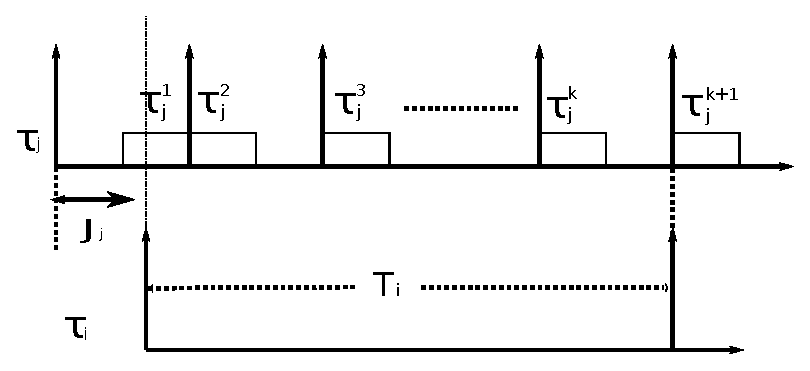
\includegraphics[bb=0bp 0bp 542bp 162bp,scale=0.5]{figures/figure9-a}
\caption{\label{fig1} Maximum interference between two tasks, running on different processors, under G-EDF}
\end{figure}


\begin{figure}
\centering
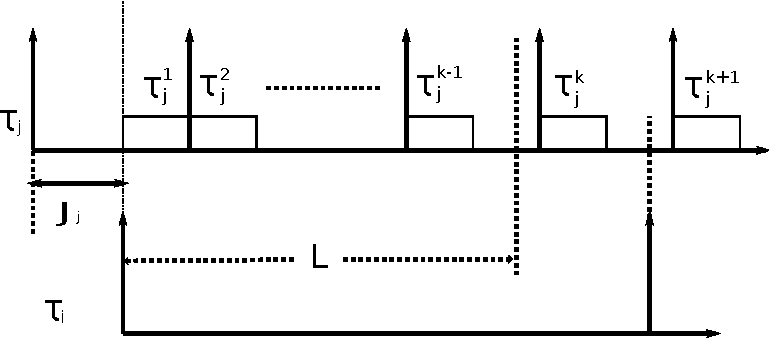
\includegraphics[bb=0bp 0bp 542bp 162bp,scale=0.5]{figures/figure9-b}
\caption{\label{fig2}Maximum interference during an interval $L$ of $T_{i}$}
\end{figure}

\subsection{Retry Cost of Atomic Sections}

\begin{figure*}
\centering
\subfigure[Early validation]{
            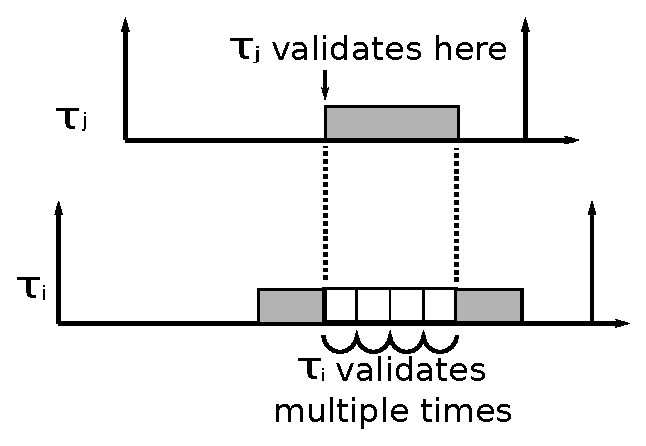
\includegraphics[scale=.45]{figures/figure5-a}
\label{fig5-a} 
}\hspace{1.2cm}
\subfigure[Lazy validation with $len(s_{i}^{k}(\theta))\le len(s_{j}^{l}(\theta))$]{
            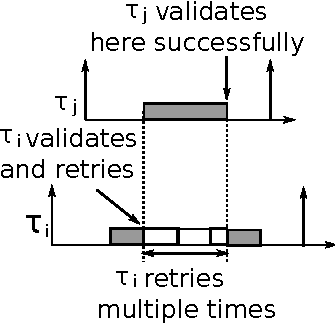
\includegraphics[scale=.65]{figures/figure5-b-1}
\label{fig5-b} 
}\hspace{1.5cm}
\subfigure[Lazy validation with $len(s_{i}^{k}(\theta))>len(s_{j}^{l}(\theta))$]{
            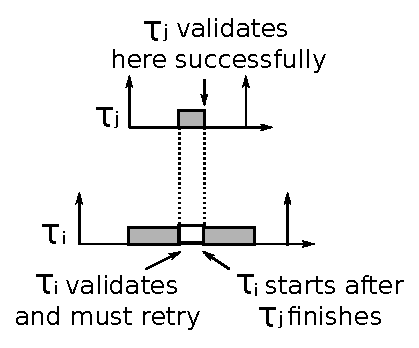
\includegraphics[scale=.65]{figures/figure5-c-1}
\label{fig5-c} 
}
\caption{Retry of $s_i^k(\theta)$ due to $s_j^l(\theta)$}  
\label{fig5}
\end{figure*}


\begin{clm}\label{gedf-edf}
Under ECM, a task $\tau_i$'s maximum retry cost during $T_i$ is upper bounded by:
%\begin{eqnarray}
%RC\left(T_{i}\right) & \le & \sum_{\theta\in\theta_{i}}\Bigg(\Big(\sum_{\tau_{j}\in\gamma_i(\theta)}\Big(\left\lceil\frac{T_{i}}{T_{j}}\right\rceil\sum_{\forall s_{j}^{l}(\theta)}len\big(s_{j}^{l}(\theta)\nonumber \\
% & + & s_{max}(\theta)\big)\Big)\Big)-s_{max}(\theta)+s_{i_{max}}(\theta)\Bigg)\label{eq3}\end{eqnarray}
 
\begin{equation}
RC\left(T_{i}\right) \le \sum_{\theta\in\theta_{i}}\left(\left(\sum_{\tau_{j}\in\gamma_i(\theta)}\left(\left\lceil\frac{T_{i}}{T_{j}}\right\rceil\sum_{\forall s_{j}^{l}(\theta)}len\left(s_{j}^{l}(\theta) + s_{max}(\theta)\right)\right)\right)-s_{max}(\theta)+s_{i_{max}}(\theta)\right)\label{eq3}\end{equation}
 
 
\end{clm}
\begin{proof}\normalfont
Consider two instances $\tau_{i}^a$ and $\tau_{j}^b$, where $d_j^b \le d_i^a$. When a shared object conflict occurs, the EDF CM will commit the atomic section of $\tau_j^b$ while aborting and retrying that of $\tau_i^a$.
Thus, an atomic section of $\tau_i^a$, $s_{i}^{k}(\theta)$,
will experience its maximum delay when it is at the end of its atomic section,  
and the conflicting atomic section of $\tau_j^b$, $s_{j}^{l}(\theta)$, starts, because the whole $s_i^k (\theta)$ will be repeated after $s_j^l (\theta)$.

Validation (i.e., conflict detection) in STM is usually done in two ways~\cite{austenmc:tcc:dissertation:2009}: a) eager (pessimistic), in which conflicts are detected at access time, and b) lazy (optimistic), in which conflicts are detected at commit time. Despite the validation time incurred (either eager or lazy),  
$s_{i}^{k}(\theta)$ will retry for the same time duration, which is $len(s_{j}^{l}(\theta)+s_i^k(\theta))$. Then, $s_i^k(\theta)$ can commit successfully  
unless it is interferred by another conflicting atomic section, as shown in Figure~\ref{fig5}. 

In Figure~\ref{fig5-a}, $s_{j}^{l}(\theta)$
validates at its beginning, due to early validation, and a conflict
is detected. So $\tau_{i}^a$ retries multiple times (because at the start of each retry, $\tau_{i}^a$ validates) 
during the execution of $s_{j}^{l}(\theta)$.
When $\tau_{j}^b$ finishes its atomic section, $\tau_{i}^a$ executes its atomic section. 

In Figure~\ref{fig5-b}, 
$\tau_{i}^a$ validates at its end (due to lazy validation), and detects a conflict with $\tau_{j}^b$.
Thus, it retries, and because its atomic section length is shorter
than that of $\tau_{j}^b$, it validates again within the execution
interval of $s_{j}^{l}(\theta)$. However, the EDF CM retries it again.
This process continues until $\tau_{j}^b$ finishes its atomic section.
If $\tau_{i}^a$'s atomic section length is longer than that of $\tau_{j}^b$,
$\tau_{i}^a$ would have incurred the same retry time, because
$\tau_{j}^b$ will validate when $\tau_{i}^a$ is retrying, and $\tau_{i}^a$ will
retry again, as shown in Figure~\ref{fig5-c}. Thus, the retry cost
of $s_{i}^{k}(\theta)$ is $len(s_{i}^{k}(\theta)+s_{j}^{l}(\theta))$.

If multiple tasks interfere with $\tau_{i}^a$ or
interfere with each other and $\tau_{i}^a$ (see the two interference examples in Figure~\ref{fig6}), then, in each case, each atomic section of the shorter deadline tasks contributes to the delay of $s_{i}^{p}(\theta)$ by its total length, plus a retry of some atomic section in the longer deadline tasks. For example,
$s_{j}^{l}(\theta)$ contributes by $len(s_{j}^{l}(\theta)+s_{i}^{p}(\theta))$
in both Figures~\ref{fig6-a} and~\ref{fig6-b}. 
%%BR: YOu should say "..in both Figures~\ref{fig6-a} and~\ref{fig6-b}." (That is, "F" must be capital case).
In Figure~\ref{fig6-b}, $s_{k}^{y}(\theta)$ causes a retry 
to $s_{j}^{l}(\theta)$, and $s_{h}^{w}(\theta)$ causes a retry to $s_{k}^{y}(\theta)$.


Since we do not know in advance which atomic section will be retried
due to another, we can safely assume that, each atomic section (that shares the same object with  $\tau_i^a$) in a shorter deadline task contributes by its total length, in addition to the maximum length between all atomic sections that share the same object, $len(s_{max}(\theta))$. Thus, 
\begin{equation}
\mbox{\ensuremath{W_{i}^{p}\left(s_{j}^{k}\left(\theta\right)\right)\le len\left(s_{j}^{k}\left(\theta\right)+s_{max}\left(\theta\right)\right)}}\label{eq2}\end{equation}


Thus, the total contribution of all atomic sections of all other tasks
that share objects with a task $\tau_i$ 
to the retry cost of $\tau_i$ during $T_i$ is:

\begin{equation}
RC\left(T_{i}\right) \le \sum_{\theta\in\theta_{i}}\sum_{\tau_{j}\in\gamma_i(\theta)}\left(\left\lceil\frac{T_{i}}{T_{j}}\right\rceil\sum_{\forall s_{j}^{l}(\theta)}len\left(s_{j}^{l}(\theta) + s_{max}(\theta)\right)\right)\label{eq3-1}\end{equation}


Here, $\left\lceil\frac{T_{i}}{T_{j}}\right\rceil\sum_{\forall s_{j}^{l}\left(\theta\right)}len\left(s_{j}^{l}\left(\theta\right)+s_{max}\left(\theta\right)\right)$ is  the contribution of all instances of $\tau_{j}$ during $T_{i}$. This contribution is added to all tasks. The last atomic section to execute is $s_{i}^{p}(\theta)$ ($\tau_i$'s atomic section that was delayed by conflicting atomic sections of other tasks). One of the other atomic sections (e.g., $s_{m}^{n}(\theta)$) should have a contribution $len(s_{m}^{n}(\theta)+s_{i_{max}}(\theta))$, instead of $len(s_{m}^{n}(\theta)+s_{max}(\theta))$. That is why one $s_{max}(\theta)$ should be subtracted, and $s_{i_{max}}(\theta)$ should be added (i.e., $s_{i_{max}}(\theta)-s_{max}(\theta)$). Claim follows.
\end{proof}

\begin{figure*}%[htbp]%
\centering%
\subfigure[Other atomic sections interfere only with $s_i^p(\theta)$]{
            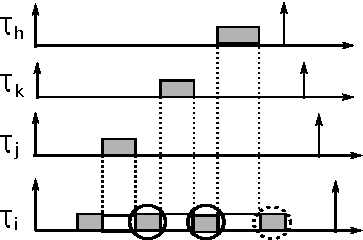
\includegraphics[scale=.65]{figures/figure6-a-1}
\label{fig6-a} 
}\hspace{1cm}
\subfigure[All atomic sections interfere with each other and $s_i^p(\theta)$]{
            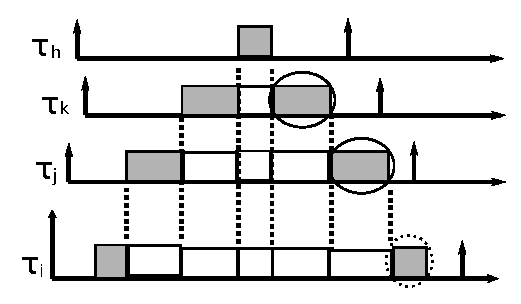
\includegraphics[scale=.6]{figures/figure6-b}
\label{fig6-b} 
}
\begin{tabular}{>{\centering}p{1cm}l}

\includegraphics[scale=0.45]{figures/circle} & Replaced in calculations by $s_{max}(\theta)$\tabularnewline

\includegraphics[scale=0.45]{figures/dotted_circle} & Replaced in calculations by $s_{i_{max}}(\theta)$\tabularnewline
\end{tabular}
\caption{Retry of $s_i^p(\theta)$ due to other atomic sections}  
\label{fig6}
\end{figure*}

\begin{clm}\label{clm:min_gedf-edf}
Claim~\ref{gedf-edf}'s retry bound can be minimized as:
\begin{equation}
RC(T_{i})\le \sum_{\theta\in\theta_{i}}min(\Phi_1 , \Phi_2)\label{eq5}\end{equation}
where $\Phi_1$ is calculated by (\ref{eq3}) for one object $\theta$ (not the sum of objects in $\theta_i$),  and 
 
\begin{equation}
\Phi_2 = \left(\sum_{\tau_{j}\in\gamma_i(\theta)} \left(\left\lceil\frac{T_{i}}{T_{j}}\right\rceil\sum_{\forall s_{j}^{l}(\theta)}len \left(s_{j}^{l}(\theta) + s_{max}^{*}(\theta) \right) \right) \right)-\bar{s}_{max}(\theta)+s_{i_{max}}(\theta)\label{eq4}\end{equation}
 
 
 where $s^*_{max}$ is the maximum atomic section between all tasks, except $\tau_j$, accessing $\theta$. $\bar{s}_{max}(\theta)$ is the second maximum atomic section between all tasks accessing $\theta$.
\end{clm}
\begin{proof}\normalfont
(\ref{eq3}) can be modified by noting that a task $\tau_j$'s atomic section 
may conflict with those of other tasks, but not with $\tau_j$. 
This is because, tasks are assumed to arrive sporadically, and  each instance finishes before the next begins. 
Thus, (\ref{eq2}) becomes:
\begin{equation}
W_i^p \left(s_j^k (\theta)\right)\le len\left(s_j^k (\theta)+s^*_{max}(\theta)\right)
\label{eq4-1}\end{equation}

To see why $\bar{s}{}_{max}(\theta)$ is used instead of $s_{max}(\theta)$, the maximum-length atomic section of each task that accesses $\theta$ is grouped into an array, in non-increasing order of their lengths. $s_{max}(\theta)$ will be the first element of this array, and $\bar{s}_{max}(\theta)$ will be the next element, as illustrated in Figure~\ref{fig7}, where the maximum atomic
section of each task that accesses $\theta$ is associated with
its corresponding task. According to (\ref{eq4-1}), all tasks
but $\tau_{j}$ will choose $s_{j_{max}}(\theta)$ as the value of $s_{max}^{*}(\theta)$.
But when $\tau_{j}$ is the one whose contribution is studied,
it will choose $s_{k_{max}}(\theta)$, as it is the maximum one not
associated with $\tau_{j}$. This way, it can be seen that the maximum
value always lies between the two values $s_{jmax}(\theta)$ and $s_{kmax}(\theta)$. 
Of course, these two values can be equal, or the maximum value can be associated with $\tau_i$ itself, and not with any one of the interfering tasks. In the latter case,
the chosen value will always be the one associated with $\tau_i$, which still lies between the two largest values. 

\begin{figure}[htbp]
\centering
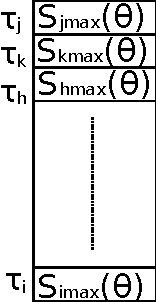
\includegraphics[scale=0.7]{figures/figure7}
\caption{\label{fig7}Values associated with $s_{max}^{*}(\theta)$}
\end{figure}


This means that the subtracted $s_{max}(\theta)$ in (\ref{eq3})
must be replaced with one of these two values ($s_{max}(\theta)$ or $\bar{s}_{max}(\theta)$). However, since we do not know  which task will interfere with $\tau_i$, the minimum is chosen, as we are determining the worst case retry cost (as this value is going to be subtracted),
and this minimum is the second maximum.

Since it is not known a-priori whether $\Phi_1$ will be smaller than $\Phi_2$ for a specific $\theta$, the minimum of $\Phi_1$ and $\Phi_2$ is taken as the worst-case contribution for $\theta$ in $RC(T_i)$. 
%Claim follows.
\end{proof}


\subsection{Upper Bound on Response Time}

To obtain an upper bound on the response time of a task $\tau_{i}$, the term $RC(T_{i})$ must be added to the workload of other tasks during the non-atomic
execution of $\tau_{i}$. But this requires modification of the WCET of each
task as follows. 

$c_{j}$ of each interfering task $\tau_{j}$ should be inflated to accommodate the interference of each task $\tau_{k},$ $k\ne j,i$. Meanwhile, atomic regions that access shared objects between $\tau_{j}$ and $\tau_{i}$ should not be considered in the inflation cost, because they have already been calculated in $\tau_{i}$'s retry cost. Thus, $\tau_{j}$'s inflated WCET becomes:
\begin{equation}
c_{ji}=c_{j}-\left(\sum_{\theta\in(\theta_{j}\wedge\theta_{i})}len \left(s_{j}(\theta) \right) \right)+RC(T_{ji})\label{eq9}\end{equation}
where, $c_{ji}$ is the new WCET of $\tau_{j}$ relative to $\tau_{i}$; 
the sum of lengths of all atomic sections in $\tau_{j}$ that access object $\theta$ is $\sum_{\theta \in (\theta_j \wedge \theta_i)} {len(s_{j}(\theta))}$; and $RC(T_{ji})$ is the $RC(T_j)$ 
 without including the shared objects between $\tau_{i}$ and $\tau_{j}$.
The calculated WCET is relative to task $\tau_{i}$, as it changes from task to task. The upper bound on the response time of $\tau_{i}$, denoted $R_{i}^{up}$, can be calculated iteratively, using a modification of Theorem 6 in~\cite{key-2}, as follows:
\begin{equation}
R_{i}^{up}=c_{i}+RC(T_{i})+\left\lfloor\frac{1}{m}\sum_{j\ne i}W_{ij}(R_{i}^{up})\right\rfloor
\label{eq10}
\end{equation}
where $R_{i}^{up}$'s initial value is $c_{i}+RC(T_{i})$.

$W_{ij}(R_{i}^{up})$ is calculated by (\ref{eq13}), and $W_{ij}(T_{i})$
is calculated by (\ref{eq11}), with $c_{j}$ replaced by 
$c_{ji}$, and changing~(\ref{eq12}) as:
\begin{equation}
W_{ij}(L)=max\begin{cases}
\left(\left\lceil\frac{L-\left(c_{ji}+\sum_{\theta\in(\theta_{j}\wedge\theta_{i})}len(s_{j}(\theta))\right)}{T_{j}}\right\rceil+1 \right)c_{ji}\\
\left\lceil\frac{L-c_{j}}{T_{j}}\right\rceil.c_{ji}+c_{j}-\sum_{\theta\in(\theta_{j}\wedge\theta_{i})}len(s_{j}(\theta))\end{cases}\label{eq14}\end{equation}

(\ref{eq14}) compares two terms, as we have two cases:


\textit{Case 1}. $\tau_j^1$ (shown in Figure~\ref{fig2}) contributes by $c_{ji}$. Thus, other instances of $\tau_j$ will begin after this modified WCET, but the sum of the shared objects' atomic section lengths is removed from $c_{ji}$, causing other instances to start earlier. Thus, the term $\sum_{\theta\in(\theta_i\wedge\theta_j)} {len(s_{j}(\theta))}$ is added to $c_{ji}$ to obtain the correct start time. 

\textit{Case 2}. $\tau_j^1$ contributes by its $c_j$, but the sum of the shared atomic section lengths  between $\tau_i$ and $\tau_j$ should be subtracted from the contribution of $\tau_j^1$, as they are already included in the retry cost. 

It should be noted that subtraction of the sum of the shared objects' atomic section lengths is done in the first case to obtain the correct start time of other instances, while in the second case, this is done to get the correct contribution of $\tau_j^1$. The maximum is chosen from the two terms in (\ref{eq14}), because they differ in the contribution of their $\tau_j^1$s, and the number of instances after that.


\subsubsection{Tighter Upper Bound}

To tighten $\tau_{i}$'s response time upper bound, $RC(\tau_i)$ needs to be calculated recursively over duration $R_i^{up}$, 
and not directly over $T_i$, as done in (\ref{eq10}). So, (\ref{eq5}) must be changed to include the modified number of interfering instances. And if $R_i^{up}$ still extends to $T_i$, a situation like that shown in Figure
\ref{fig10} can happen.
\begin{figure}
\centering{}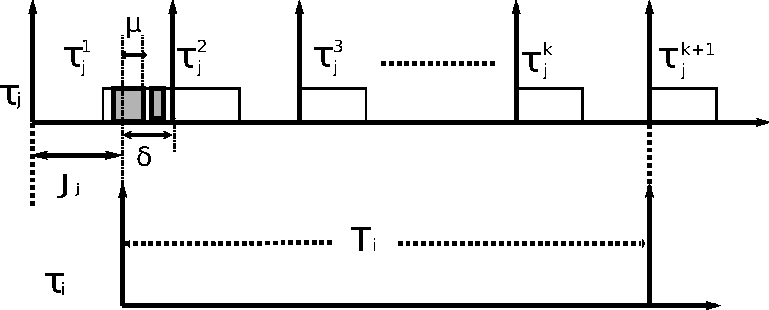
\includegraphics[scale=0.5]{figures/figure10}\caption{\label{fig10} Atomic sections of job $\tau_{j}^{1}$ contributing to period $T_i$}
\end{figure}


To counter the situation in Figure~\ref{fig10}, atomic sections of $\tau_{j}^{1}$ that are contained in the interval $\delta$
are the only ones that can contribute to $RC(T_{i})$. Of course, they can be lower, but cannot be greater, because $\tau_{j}^{1}$ has been delayed by its maximum jitter. Hence, no more atomic sections
can interfere during the duration 
$[d_j^1 -\delta,d_j^1]$.

For simplicity, we use the following notations:
\begin{compactitem}
\item $\lambda_{1}\left(j,\theta\right)=\sum_{\forall s_{j}^{l}\left(\theta\right)\in\left[d_j^1-\delta,d_j^1\right]}len\left(s_{j}^{l^{*}}\left(\theta\right)+s_{max}\left(\theta\right)\right)$
\item $\chi_{1}\left(i,j,\theta\right)=\left\lfloor\frac{T_{i}}{T_{j}}\right\rfloor\sum_{\forall s_{j}^{l}\left(\theta\right)}len\left(s_{j}^{l}\left(\theta\right)+s_{max}\left(\theta\right)\right)$
\item $\lambda_{2}\left(j,\theta\right)=\sum_{\forall s_{j}^{l}\left(\theta\right)\in\left[d_{j}^{1}-\delta,d_{j}^{1}\right]}len\left(s_{j}^{l^{*}}\left(\theta\right)+s_{max}^{*}\left(\theta\right)\right)$
\item $\chi_{2}\left(i,j,\theta\right)=\left\lfloor\frac{T_{i}}{T_{j}}\right\rfloor\sum_{\forall s_{j}^{l}\left(\theta\right)}len\left(s_{j}^{l}\left(\theta\right)+s_{max}^{*}\left(\theta\right)\right)$
\end{compactitem}
Here, $s_{j}^{l^{*}}\left(\theta\right)$ is the part of $s_{j}^{l}\left(\theta\right)$ that
is included in the interval $\delta$. Thus, if $s_j^l (\theta)$ is partially included in $\delta$, it contributes by its included length $\mu$.

Now, (\ref{eq5}) can be modified as:
\begin{equation}
RC\left(T_{i}\right)\le \sum_{\theta\in\theta_{i}}min\begin{cases}
\begin{cases}
\Bigl(\left(\sum_{\tau_{j}\in\gamma_i\left(\theta\right)}\lambda_{1}\left(j,\theta\right)+\chi_{1}\left(i,j,\theta\right)\right)\\
-s_{max}\left(\theta\right)+s_{i_{max}}\left(\theta\right)\Bigr)\end{cases}\\
\begin{cases}
\Bigl(\left(\sum_{\tau_{j}\in\gamma_i\left(\theta\right)}\lambda_{2}\left(j,\theta\right)+\chi_{2}\left(i,j,\theta\right)\right)\\
-\bar{s}_{max}\left(\theta\right)+s_{i_{max}}\left(\theta\right)\Bigr)\end{cases}\end{cases}\label{eq15}\end{equation}



Now, we compute $RC(L)$, where $L$ does not extend to the last instance of $\tau_{j}$. Let:
\begin{compactitem}
\item $\upsilon\left(L,j\right)=\left\lceil\frac{L-c_{j}}{T_{j}}\right\rceil+1$
\item $\lambda_{3}\left(j,\theta\right)=\sum_{\forall s_{j}^{l}\left(\theta\right)}len\left(s_{j}^{l}\left(\theta\right)+s_{max}\left(\theta\right)\right)$
\item $\lambda_{4}\left(j,\theta\right)=\sum_{\forall s_{j}^{l}\left(\theta\right)}len\left(s_{j}^{l}\left(\theta\right)+s_{max}^{*}\left(\theta\right)\right)$
\end{compactitem}
Now, (\ref{eq5}) becomes: 
\begin{equation}
RC\left(L\right)\le \sum_{\theta\in\theta_{i}}min\begin{cases}
\begin{cases}
\left(\sum_{\tau_{j}\in\gamma_i\left(\theta\right)}\left(\upsilon\left(L,j\right)\lambda_{3}\left(j,\theta\right)\right)\right)\\
-s_{max}\left(\theta\right)+s_{i_{max}}\left(\theta\right)\end{cases}\\
\begin{cases}
\left(\sum_{\tau_{j}\in\gamma_i\left(\theta\right)}\left(\upsilon\left(L,j\right)\lambda_{4}\left(j,\theta\right)\right)\right)\\
-\bar{s}_{max}\left(\theta\right)+s_{i_{max}}\left(\theta\right)\end{cases}\end{cases}\label{eq16}\end{equation}


Thus, an upper bound on $RC(\tau_i)$ is given by:
\begin{equation}
RC(R_{i}^{up})\le min\begin{cases}
RC(R_{i}^{up})\\
RC(T_{i})\end{cases}
\label{eq17}
\end{equation}
where $RC(R_i^{up})$ is calculated by~(\ref{eq16}) if $R_i^{up}$ does not extend to the last interfering instance of $\tau_j$; otherwise, it is calculated by~(\ref{eq15}). The final upper bound on $\tau_{i}$'s response time can be calculated
as in (\ref{eq10}) by replacing $RC(T_{i})$ with
$RC(R_{i}^{up})$.



\section{RCM}
\label{sec:g-rma-rma-cm}

As G-RMA is a fixed priority scheduler,  a task $\tau_{i}$ will be interfered by those tasks with priorities higher than $\tau_{i}$ (i.e., $p_{j}>p_{i}$).  Upon a conflict, the RMA CM will commit the transaction that belongs to the higher priority task. Hereafter, we use \emph{RCM} to refer to a multicore system scheduled by G-RMA and resolves STM conflicts by the RMA CM. RCM is shown in Alogrithm~\ref{rcm_algorithm}.
\begin{algorithm}
\footnotesize{
\LinesNumbered
\KwData{$s_i^k(\theta)\rightarrow$ interfered atomic section. $s_j^l(\theta)\rightarrow$ interfering atomic section}
\KwResult{which atomic section aborts}
\eIf{$T_i < T_j$}
	{$s_j^l(\theta)$ aborts\label{rcm:step_sicommits}\;}
	{$s_i^k(\theta)$ aborts\label{rcm:step_siaborts}\;}
	}
\caption{RCM}
\label{rcm_algorithm}
\end{algorithm}

The same illustrative example in Section~\ref{ecm_illustrative_ex} is applied for RCM except that tasks' priorities are fixed.

\subsection{Maximum Task Interference}

Figure~\ref{fig11} illustrates the maximum interference caused by a task $\tau_{j}$
to a task $\tau_{i}$ under G-RMA. As $\tau_{j}$ is of higher priority than $\tau_{i}$,
$\tau_{j}^{k}$ will interfere with $\tau_{i}$ even if it is not totally
included in $T_{i}$. Unlike the G-EDF case shown in Figure~\ref{fig10}, 
where only the $\delta$ part of $\tau_{j}^{1}$ is considered, in G-RMA,
$\tau_{j}^{k}$ can contribute by the whole $c_{j}$, and all atomic
sections contained in $\tau_{j}^{k}$ must be considered. This is because, in G-EDF, the worst-case pattern releases $\tau_{i}^a$ before $d_{j}^{1}$
by $\delta$ time units, and $\tau_{i}^a$ cannot be interfered before it
is released. But in G-RMA, $\tau_{i}^a$ is already released, and can be
interfered by the whole $\tau_{j}^{k}$, even if this makes it infeasible.


\begin{figure}[htbp]
\centering
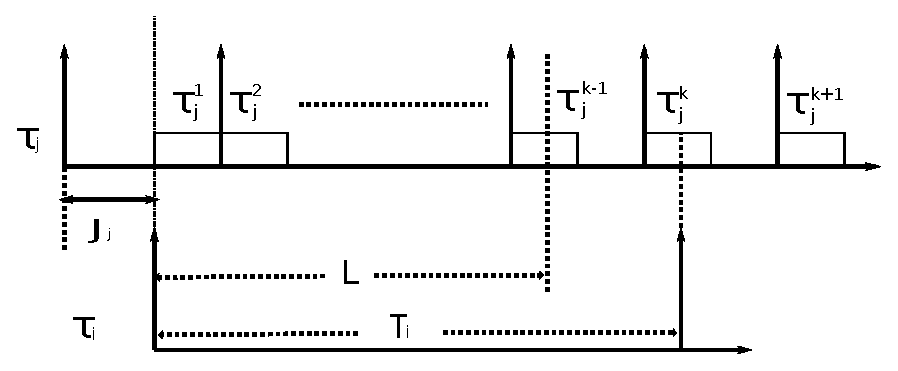
\includegraphics[scale=0.5]{figures/figure11}\caption{\label{fig11}Max interference of $\tau_{j}$ to $\tau_{i}$ in G-RMA}
%%BR: $T_{j}$ and $T_{i}$ are task periods. Is that what you meant here?
\end{figure}

Thus, the maximum contribution of $\tau_{j}^b$ to $\tau_{i}^a$ for any duration
$L$ can be deduced from Figure~\ref{fig11} as $W_{ij}(L)=\left(\left\lceil\frac{L-c_{j}}{T_{j}}\right\rceil+1 \right)c_{j}$,
where $L$ can extend to $T_{i}$. Note the contrast with ECM, where $L$ cannot be extended directly to $T_i$, as this will have a different pattern of worst case interference from other tasks.

\subsection{Retry Cost of Atomic Sections}

\begin{clm}\label{clm:rcm_retry_cost}
Under RCM, a task $\tau_i$'s retry cost over duration $L$, which can extend to $T_i$, is upper bounded by:
%\begin{eqnarray}
%RC\left(L\right) & \le & \sum_{\theta\in\theta_{i}}\Bigg(\left(\sum_{\tau_{j}^{*}}\left(\left(\left\lceil\frac{L-c_{j}}{T_{j}}\right\rceil+1\right)\pi\left(j,\theta\right)\right)\right)\nonumber \\
% & - & s_{max}^{min}\left(\theta\right)+s_{i_{max}}\left(\theta\right)\Bigg)\label{eq20}\end{eqnarray}
 
\begin{equation}
RC\left(L\right) \le sum_{\theta\in\theta_{i}}\left(\left(\sum_{\tau_{j}^{*}}\left(\left(\left\lceil\frac{L-c_{j}}{T_{j}}\right\rceil+1\right)\pi\left(j,\theta\right)\right)\right) - s_{max}^{min}\left(\theta\right)+s_{i_{max}}\left(\theta\right)\right)\label{eq20}\end{equation} 
 
 where:
 \begin{compactitem}
\item $\tau_{j}^{*}=\{\tau_{j}|(\tau_{j}\in\gamma_i(\theta))\wedge(p_{j}> p_{i})\}$
\item $\pi(j,\theta)=\sum_{\forall s_{j}^{l}(\theta)}len\left(s_{j}^{l}\left(\theta\right)+s_{max}^{j}\left(\theta\right)\right)$
\item $s_{max}^{min}(\theta)=min_{\forall \tau_j^*} \{s_{max}^j(\theta) \in \tau_k \}$, where $p_j > p_k > p_i$
\end{compactitem}
\end{clm}
\begin{proof}\normalfont
The worst case interference pattern for RCM is the same as that for ECM for an interval $L$, except that, in RCM, $L$ can extend to the entire $T_i$, but in ECM, it cannot, as the interference pattern of $\tau_j$ to $\tau_i$ changes. 
Thus, (\ref{eq16}) can be used to calculate $\tau_i$'s retry cost, with some modifications, as we do not have to obtain the minimum of the two terms in (\ref{eq16}), because $\tau_j$'s atomic sections will abort and retry only atomic sections of tasks with lower priority than $\tau_j$. Thus, $s_{max}(\theta)$, $s_{max}^*(\theta)$, and $\bar{s}_{max}(\theta)$ are replaced by $s_{max}^{min}(\theta)$, which is the minimum of the set of maximum-length atomic sections of tasks with priority lower than $\tau_j$ and share object $\theta$ with $\tau_i$. This is because, the maximum length atomic section of tasks other than $\tau_j$ differs according to $j$. Besides, as $\tau_i$'s atomic sections can be aborted only by atomic sections of higher priority tasks, not all $\tau_j \in \gamma (\theta)$ are considered, but only the subset of tasks in $\gamma (\theta)$ with priority higher than $\tau_i$ (i.e., $\tau_j^*$). 
Claim follows.
\end{proof}



\subsection{Upper Bound on Response Time}

The response time upper bound can be computed using Theorem 7 in~\cite{key-2} with a modification to include the effect of retry cost. The upper bound is given by:
\begin{equation}
R_{i}^{up}=c_{i}+RC(R_{i}^{up})+\left\lfloor\frac{1}{m}\sum_{j\ne i}W_{ij}(R_{i}^{up})\right\rfloor\label{eq22}\end{equation}
where $W_{ij}(R_{i}^{up})$ is calculated as in (\ref{eq14}), $c_{ji}$ is calculated by (\ref{eq9}), and $RC$ is calculated by (\ref{eq20}).

%%BR: Skipped reviewing the following %%%%%%%%%%%%%
\begin{comment}
\section{FMLP and OMLP Blocking Times}
\label{sec:blocking-bound-fmlp-omlp}

The FMLP protocol~\cite{brandenburg2008comparison} has been shown to be superior to other multicore real-time locking protocols in terms of schedulability, and the global OMLP protocol~\cite{key-3} has been shown to be asymptotically optimal. To formally compare STM against FMLP and global OMLP, we first upper bound their blocking times. %(those were not presented in~\cite{brandenburg2008comparison,key-4,key-3}). 


\subsection{\label{global-fmlp}Global FMLP}

FMLP can be used with global and partitioned scheduling. Since we only consider global scheduling, ``FMLP" and ``global FMLP" mean the same, for the paper's purpose.


FMLP divides shared objects into short resources, $s\_\theta$, and long ones, $l\_\theta$. Nested resources 
are grouped together into two groups: $g(s\_\theta)$ that contains only short resources, and $g(l\_\theta)$ that contains only long resources.
A request $R_i (g(s\_\theta))$ is made by a task $T_i$ to access one or more resources in $g(s\_\theta)$. This request's length is denoted $|R_i (g(s\_\theta))|$, and the number of times $T_i$ requests short resources is denoted $N_{i,s}$. Similarly, $R_i (g(l\_\theta))$ is $T_i$'s request to a group containing long resources for a duration $|R_i (g(l\_\theta))|$, and $N_{i,l}$ is the number of times $T_i$ requests long resources.


Global FMLP uses a variant of G-EDF (called GSN-EDF which discriminates between
linked jobs and scheduled ones) to account for non-preemptive jobs while still using G-EDF for scheduling, 
%%BR: "jobs"?? (can there be multiple linked jobs)?
%%BR: "ones"?? (can there be multiple scheduled ones)?
Tasks busy-wait on short resources, and suspend on long ones. In both cases, requests for resources are arranged in FIFO queues, 
%%BR: "FIFO queue" or "FIFO queues"???? (since there are two resource types)
and for requesting long resources, the task holding the resource inherits the highest priority of the suspended tasks on that resource. For short resources, there is no need to inherit priorities, as tasks become non-preemptable when acquiring short resources. 

Requests for long resources can contain requests for the short resource group, but the reverse is not true. The protocol allows non-preemptable jobs and bounds the time a job is non-preemptively blocked by a lower priority job as the maximum time a non-preemptive section of the job can be linked to the processor of the higher priority job. This non-preemptive blocking can only happen when the higher priority job is released or resumed.


Three types of blocking can be incurred by any task under global FMLP. These include busy-wait blocking, non-preemptive blocking, and direct blocking. The total blocking time of a job, $b_{i}$, is the sum of these three blocking durations. Execution time of each task, $e_{i}$, is inflated by this blocking amount ($e_{i}+b_{i}$), and is used in any of the G-EDF schedulability tests (e.g.,~\cite{Goossens:2003:PSP:876600.876615,srinivasan2002deadline}) 
for verifying schedulability. 

We upper bound a task's blocking durations due to busy-wait blocking, non-preemptive blocking, and direct blocking, denoted as $BW(T_{i})$, $NPB(T_{i})$, and $DB(T_{i})$, respectively, as follows.  
(Note that, in~\cite{key-3}, no upper bounds are presented for these terms, except for $DB(T_{i})$, as~\cite{key-3}'s main focus is on FMLP's suspension-based part. Also, the upper bound for $DB(T_{i})$ in~\cite{key-3} does not consider the effect of requesting a short resource within a long one.)


A job $T_{i}^{j}$ busy-waits in a FIFO queue when it is scheduled on a processor and it cannot be removed by any other task until its request is satisfied. As busy-waiting tasks are non-preemptable, job $T_{i}^{j}$ can be blocked for at most the maximum $m-1$ requests, where each request consists of the sum of the nested requests
to some resources in the same group. This process proceeds for each short resource requested by $T_{i}$. The busy-wait blocking time, $BW(T_{i})$, is therefore:
\begin{equation}
BW(T_{i})\le\sum_{s\_\theta\in\theta_{i}} \left(max \left[\sum_{k=1,k\ne i}^{min(m,n)-1} \left| R_{k} \left(g \left(s\_\theta \right) \right) \right| \right] \right)\label{eq26}
\end{equation}

A job $T_{i}^{j}$ can be non-preemptively blocked, either at its release or when it resumes, by at most the maximum (nested) request to any short resource. The non-preemptive blocking time, $NPB(T_{i})$, is therefore:
\begin{equation}
NPB(T_{i})=(1+N_{i,l}).max_{k\ne i} \left| R_{k}(g(s\_\theta)) \right|\label{eq27}
\end{equation}
Here, $1$ is added to $N_{i,l}$, because $T_{i}$ can be non-preemptively blocked at its release, in addition to suspension times. 

A job $T_{i}^{j}$ can be blocked by all other $n-1$ tasks for any long resource. Any of these $n-1$ requests can be a nested request to long resources belonging to the same group. In addition, any of those requests can contain a request to a short resource, and so it can busy-wait on it. Thus, each request in the $n-1$ requests, requiring access to a short resource, can be delayed by at most the maximum $m-1$ requests to the group containing that short resource. The direct blocking time, $DB(T_{i})$, is therefore:
\begin{equation}
DB(T_{i})\le\sum_{l\_\theta\in\theta_{i}} \left[max_{k=1,k\ne i}^{n-1} \left|R_{k} \left(g \left(l\_\theta \right) \right) \right| \right]
\label{eq28}
\end{equation}


\subsection{Global OMLP}


In~\cite{key-3}, 
global FMLP has a maximum s-oblivious pi-blocking cost of $\Theta(n)$, whereas global OMLP~\cite{key-3}, which is a suspension-based protocol that supports G-EDF, as well as any global job-level static priority (JLSP) scheduler, has a $\Theta(m)$ s-oblivious pi-blocking cost, as seen by equation (\ref{eq29}):
\begin{equation}
b_{i}\triangleq\sum_{k=1}^{q}N_{i,k}.2.(m-1).max_{1\le i\le n}\{L_{i,k}\}\label{eq29}\end{equation}
where $N_{i,k}$ is the maximum number of times $T_i$ requests resource $k$, and $L_{i,k}$ is the maximum execution time of such a request. $N_{i,k}$ and $L_{i,k}$ are assumed to be constants,
so the s-oblivious pi-blocking is $\Theta(m)$, and thus it is optimal.
\end{comment}

%%BR: Resumed editing from here
\section{STM versus Lock-Free}
\label{sec:comparison}

We now would like to understand when STM will be beneficial compared to lock-free synchronization. The retry-loop lock-free approach in~\cite{key-5} is the most relevant to our work. 


\subsection{\label{sub:G-EDF-scheduler-with}ECM versus Lock-Free}

\begin{clm}
For ECM's schedulability to be better or equal to that of~\cite{key-5}'s retry-loop lock-free approach,  
the size of $s_{max}$ must not exceed one half of that of $r_{max}$, where $r_{max}$ is the maximum execution cost of a single iteration of any lock-free retry loop of any task. With low number of conflicting tasks, the size of $s_{max}$ can be at most the size of $r_{max}$. 
\end{clm}
\begin{proof}\normalfont
Equation (\ref{eq17}) can be upper bounded as:
\begin{equation}
RC\left(T_{i}\right) \le \sum_{\tau_{j}\in\gamma_{i}}\left(\sum_{\theta\in\theta_{i}}\left(\left\lceil\frac{T_{i}}{T_{j}}\right\rceil\sum_{\forall s_{j}^{l}\left(\theta\right)}\left(2.s_{max}\right)\right)\right)
\label{eq30}
\end{equation}
where $s_{j}^{l}\left(\theta\right)$, $s_{i_{max}}\left(\theta\right)$,
$s_{max}^{*}\left(\theta\right)$, and $\bar{s}_{max}\left(\theta\right)$ are replaced by $s_{max}$, and the order of the first two summations are reversed
by each other, 
with $\gamma_{i}$ being the set of tasks that share objects
with $\tau_{i}$. These changes are done to simplify the comparison.

Let $\sum_{\theta\in\theta_{i}}\sum_{\forall s_{j}^{l}\left(\theta\right)}=\beta_{i,j}^{*}$, and $\alpha_{edf}=\sum_{\tau_{j}\in\gamma_{i}}\left\lceil\frac{T_{i}}{T_{j}}\right\rceil.2\beta_{i,j}^*$. Now, (\ref{eq30}) can be modified as:
\begin{equation}
RC\left(T_{i}\right)=\alpha_{edf}.s_{max}
\label{eq31}
\end{equation}

The loop retry cost is given by:
\begin{eqnarray}
LRC\left(T_i\right)&=&\sum_{\tau_{j}\in\gamma_{i}}\left(\left\lceil\frac{T_{i}}{T_{j}}\right\rceil+1\right).\beta_{i,j}.r_{max}\nonumber \\
&=& \alpha_{free} . r_{max} \label{eq32}
\end{eqnarray}
where $\beta_{i,j}$ is the number of retry loops of $\tau_{j}$ that accesses the same object as that accessed by some retry loop of $\tau_{i}$, and $\alpha_{free} = \sum_{\tau_{j}\in\gamma_{i}}\left(\left\lceil\frac{T_{i}}{T_{j}}\right\rceil + 1 \right).\beta_{i,j}$.
Since the shared objects are the same in both STM and lock free, $\beta_{i,j}=\beta_{i,j}^{*}$.
Thus, STM achieves equal or better schedulability 
than lock-free if the total utilization of the STM system is less than or equal to that of the lock-free system:
\begin{eqnarray}
\sum_{\tau_{i}}\frac{c_{i}+\alpha_{edf}.s_{max}} {T_{i}} & \le & \sum_{\tau_{i}}\frac{c_{i}+\alpha_{free}.r_{max}}{T_{i}} \nonumber \\
\therefore\frac{s_{max}}{r_{max}} & \le & \frac{\sum_{\tau_{i}}\alpha_{free}/T_{i}}{\sum_{\tau_{i}}\alpha_{edf}/T_{i}}\end{eqnarray}


Let $\bar{\alpha}_{free}=\sum_{\tau_{j}\in\gamma_{i}}\left\lceil\frac{T_{i}}{T_{j}}\right\rceil.\beta_{i,j}$,  $\hat{\alpha}_{free}=\sum_{T_{j}\in\gamma_{i}}\beta_{i,j}$, and $\alpha_{free}=\bar{\alpha}_{free}+\hat{\alpha}_{free}.$ Therefore: 
\begin{eqnarray}
\frac{s_{max}}{r_{max}} & \le & \frac{\sum_{\tau_{i}}(\bar{\alpha}_{free} +\hat{\alpha}_{free})/T_{i}}{\sum_{\tau_{i}}\alpha_{edf}/T_{i}}\nonumber \\
 & = & \frac{1}{2}+\frac{\sum_{\tau_{i}}\hat{\alpha}_{free} /T_{i}}{\sum_{\tau_{i}}\alpha_{edf}/T_{i}}
 \label{eq33}
 \end{eqnarray}

Let $\zeta_{1}=\sum_{\tau_{i}}\hat{\alpha}_{free}/T_{i}$
and $\zeta_{2}=\sum_{\tau_{i}}\left(\frac{\alpha_{edf}}{2}\right)/T_{i}$. The maximum value of $\frac{\zeta_{1}}{2.\zeta_{2}}=\frac{1}{2}$, which can happen if $T_{j}\ge T_{i}\,\therefore\left\lceil\frac{T_{i}}{T_{j}}\right\rceil=1$. Then (\ref{eq33})=$1$, which is its maximum value. $T_{j}\ge T_{i}$ means that there is a small number of interferences from other tasks
to $\tau_{i}$, and thus low number of conflicts. Therefore, $s_{max}$ is
allowed to be as large as $r_{max}$.

The theoretical minimum value for $\frac{\zeta_{1}}{2.\zeta_{2}}$
is $0$, which can be asymptotically reached if $T_{j}\ll T_{i}$,
$\therefore\,\left\lceil\frac{T_{i}}{T_{j}}\right\rceil\rightarrow\infty$
and $\zeta_{2}\rightarrow\infty$. Thus, (\ref{eq33})$\rightarrow1/2$.

$\beta_{i,j}$ has little effect on $s_{max}/r_{max}$, 
as it is contained in both the numerator and denominator. Irrespective of whether $\beta_{i,j}$ is going to reach its maximum or minimum value, both can be considered constants, and thus removed from (\ref{eq33})'s numerator and denominator. 
However, the number of
interferences of other tasks to $\tau_{i}$, $\left\lceil\frac{T_{i}}{T_{j}}\right\rceil$,
has the main effect on $s_{max}/r_{max}$. This is illustrated in Figure~\ref{fig14}. Claim follows.
\end{proof}

\begin{figure}
\begin{centering}
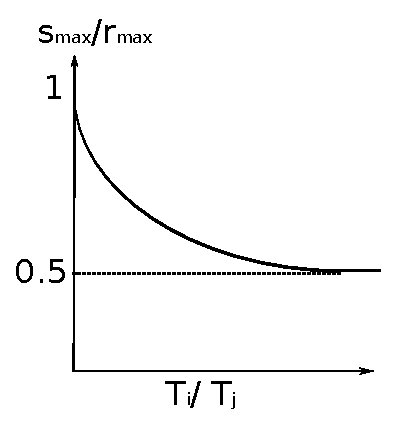
\includegraphics[scale=0.5]{figures/figure14}
\par\end{centering}
\caption{\label{fig14}Effect of $\left\lceil\frac{T_{i}}{T_{j}}\right\rceil$ on
$\frac{s_{max}}{r_{max}}$}
\end{figure}

%%BR: Stopped here. 3:32PM, 10/18/11.

\subsection{RCM versus Lock-Free}

\begin{clm}
For RCM's schedulability to be better or equal to that of~\cite{key-5}'s retry-loop lock-free approach, the size of $s_{max}$ must not exceed one half of that of $r_{max}$ for all cases.
However, the size of $s_{max}$ can be larger than that of $r_{max}$, depending on the number of accesses to a task $T_i$'s shared objects from other tasks.
\end{clm}
\begin{proof}\normalfont
Equation (\ref{eq20}) is upper bounded by:
 \begin{equation}
\sum_{\left(\tau_{j}\in\gamma_{i}\right)\wedge\left(p_{j}> p_{i}\right)}\left(\left\lceil\frac{T_{i}-c_{j}}{T_{j}}\right\rceil+1\right).2.\beta_{i,j}.s_{max}
\label{eq34}\end{equation}

Consider the same assumptions as in Section~\ref{sub:G-EDF-scheduler-with}.
Let $\alpha_{rma}=\sum_{\left(\tau_{j}\in\gamma_{i}\right)\wedge\left(p_{j}> p_{i}\right)}\left(\left\lceil\frac{T_{i}-c_{j}}{T_{j}}\right\rceil+1\right).2.\beta_{i,j}$. Now, the ratio $s_{max}/r_{max}$ is upper bounded by:
\begin{equation}
\frac{s_{max}}{r_{max}}\le\frac{\sum_{T_{i}}\alpha_{free}/t\left(T_{i}\right)}{\sum_{T_{i}}\alpha_{rma}/t\left(T_{i}\right)}
\label{eq35}\end{equation}

The main difference between RCM and lock-free is that RCM is affected only by the higher priority tasks, while lock-free is affected by all tasks (just as in ECM). 
Besides, RCM
is still affected by $2.\beta_{i,j}$ (just as in ECM).
The subtraction of $c_{j}$ in the numerator of (\ref{eq34}) may not
have a significant effect on the ratio of (\ref{eq35}), as the loop retry 
cost can also be modified to account for the effect of the first interfering
instance of task $T_{j}$. Therefore, 
$\alpha_{free} = \sum_{\tau_{j}\in\gamma_{i}}\left(\left\lceil\frac{T_{i}-c_j}{T_{j}}\right\rceil + 1 \right)\beta_{i,j}$.

Let tasks in the denominator of (\ref{eq35}) be given indexes $k$ instead of $i$, and $l$ instead of $j$. Let tasks in both the numerator and denominator of (\ref{eq35}) be arranged in the non-increasing priority order, so that $i=k$ and $j=l$. Let $\alpha_{free}$ in (\ref{eq35}) be divided into two parts: $\bar{\alpha}_{free}$ that contains only tasks with priority higher than $\tau_i$, and $\hat{\alpha}_{free}$ that contains only tasks with priority lower than $\tau_i$. Now, (\ref{eq35}) becomes:
\begin{eqnarray}
\frac{s_{max}}{r_{max}} & \le & \frac{\sum_{\tau_{i}}(\bar{\alpha}_{free}+\hat{\alpha}_{free})/T_{i}}{\sum_{\tau_{k}}\alpha_{rma}/T_{k}}\nonumber \\
 & = & \frac{1}{2}+\frac{\sum_{\tau_{i}}\hat{\alpha}_{free}/T_{i}}{\sum_{\tau_{k}}\alpha_{rma}/T_{k}}\label{eq36}\end{eqnarray}

For convenience, we introduce the following notations:
\begin{eqnarray}
\zeta_{1}& = & \sum_{\tau_{i}}\frac{\sum_{\left(\tau_{j}\in\gamma_{i}\right)\wedge\left(p_{j}<p_{i}\right)}\left(\left\lceil\frac{T_{i}-c_{j}}{T_{j}}\right\rceil+1\right)\beta_{i,j}}{T_{i}}\nonumber\\
& = & \sum_{T_i} \hat{\alpha}_{free}/T_i
\nonumber\\
\zeta_{2} 
& = & \sum_{\tau_{k}}\frac{\sum_{\left(\tau_{l}\in\gamma_{k}\right)\wedge\left(p_{l}>p_{k}\right)}\left(\left\lceil\frac{T_{k}-c_{l}}{T_{l}}\right\rceil+1\right)\beta_{k,l}}{T_{k}}\nonumber\\
& = & \frac{1}{2}\sum_{\tau_k} \alpha_{rma}/T_k\nonumber
\end{eqnarray}
$\tau_{j}$ is of lower priority than $\tau_{i}$, which means $D_{j}>D_{i}$. Under G-RMA, this means, $T_{j}>T_{i}$.
Thus, $\left\lceil\frac{T_{i}-c_{j}}{T_{j}}\right\rceil=1$ for
all $\tau_{j}$ and $\zeta_{1}=\sum_{\tau_{i}}(\sum_{(\tau_{j}\in\gamma_{i})\wedge(p_{j}<p_{i})}(2.\beta_{i,j}))/T_{i}$.
Since $\zeta_{1}$ contains all $\tau_{j}$ of lower priority than
$\tau_{i}$ and $\zeta_{2}$ contains all $\tau_{l}$ of higher priority than $\tau_{k}$, 
and tasks are arranged in the non-increasing priority order, then for each $\tau_{i,j}$, there exists $\tau_{k,l}$ such
that $i=l$ and $j=k$. Figure~\ref{fig:matrix-example} illustrates this, where 0 means that the pair $i,j$ 
does not exist in $\zeta_{1}$,
and the pair $k,l$ does not exist in $\zeta_{2}$' (i.e., 
there is no task $\tau_l$ that will interfere with $\tau_k$ in $\zeta_2$), 
and 1 means the opposite. 

\begin{figure}[htbp]
\centering
\begin{tabular}{ccc}
$\begin{array}{cccccc}
 & j & 1 & 2 & \cdots & n\\
i\\
1 &  & 0 & 1 & \cdots & 1\\
2 &  & 0 & 0 & \ddots & \vdots\\
\vdots &  & \vdots & \vdots & \ddots & 1\\
n &  & 0 & 0 & \cdots & 0\end{array}$ &  & $\begin{array}{cccccc}
 & l & 1 & 2 & \cdots & n\\
k\\
1 &  & 0 & 0 & \cdots & 0\\
2 &  & 1 & 0 &  & \vdots\\
\vdots &  & \vdots & \ddots & \ddots & 0\\
n &  & 1 & \cdots & 1 & 0\end{array}$\tabularnewline
\end{tabular}
\caption{\label{fig:matrix-example} Task association for lower priority tasks than $T_i$ and higher priority tasks than $T_k$}
\end{figure}


Thus, it can be seen that both the matrices are transposes of
each other. Consequently, for each $\beta_{i,j}$, there exists $\beta_{k,l}$
such that $i=l$ and $j=k$. But the number of times $\tau_{j}$ accesses
a shared object with $\tau_{i}$ may not be the same as the number of times
$\tau_{i}$ accesses that same object. Thus, $\beta_{i,j}$ does not have
to be the same as $\beta_{k,l}$, even if $i,j$ and $k,l$ are transposes 
of each other. Therefore, we can analyze the behavior of $s_{max}/r_{max}$ based on the three parameters $\beta_{i,j}$, $\beta_{k,l}$, and $\left\lceil\frac{T_{k}-c_{l}}{T_{l}}\right\rceil$.
If $\beta_{i,j}$ is increased so that $\beta_{i,j}\rightarrow\infty$,
$\therefore\,$(\ref{eq36})$\rightarrow\infty$.
This is because, $\beta_{i,j}$ represents the number of times a lower priority task $\tau_{j}$ accesses 
shared objects with a higher priority task $\tau_{i}$. 
While this number has a greater effect in lock-free, it does not have any effect under RCM, because lower priority tasks do not affect higher priority
ones. Hence, $s_{max}$ is allowed to be much greater than $r_{max}$.

Although the minimum value for $\beta_{i,j}$ is 1, mathematically, if $\beta_{i,j}\rightarrow0$, then (\ref{eq36}) 
 $\rightarrow1/2$.
Here, changing $\beta_{i,j}$ does not affect the retry cost of RCM, but it does affect the retry cost of lock-free, because the contention between tasks is reduced. Thus, $s_{max}$ is reduced in this case to
a little more than half of $r_{max}$ (``a little more''
because the minimum value of $\beta_{i,j}$ is actually 1, not 0).


The change of $s_{max}/r_{max}$ with respect to $\beta_{i,j}$ is illustrated in Figure~\ref{fig15-a}.
If $\beta_{k,l}\rightarrow\infty$, then (\ref{eq36}) $\rightarrow1/2$.
This is because, $\beta_{k,l}$ represents the number of times 
a higher priority task $\tau_{l}$ accesses shared objects with a lower
priority task $\tau_{k}$. Under RCM, this will increase the retry 
cost, thus reducing $s_{max}/r_{max}$. But if $\beta_{k,l}\rightarrow0$, then (\ref{eq36})$\rightarrow\infty$. This is due to the lower contention from a higher priority task $\tau_{l}$ to a lower priority task $\tau_{k}$, which reduces the retry cost under RCM and allows $s_{max}$ to be very large compared with $r_{max}$. Of course, the actual minimum value for $\beta_{k,l}$ is 1, and is illustrated in Figure~\ref{fig15-b}.

%%%%%%

The third parameter that affects $s_{max}/r_{max}$ is $T_{k}/T_{l}$.
If $T_{l}\ll T_{k}$, then $\left\lceil\frac{T_{k}-c_{l}}{T_{l}}\right\rceil\rightarrow\infty$,
and (\ref{eq36}) $\rightarrow1/2$. This is due to a high number
of interferences from a higher priority task $\tau_{l}$ to a lower priority
task $\tau_{k}$, which increases the retry cost under RCM, 
%%BR: WHy don't you say "RCM"? Fix it. 
and consequently reduces $s_{max}/r_{max}$. 

If $T_{l}=T_{k}$ (which is
the maximum value for $T_{l}$ as $D_{l}\le D_{k}$, because
$\tau_{l}$ has a higher priority than $\tau_{k}$), then $\left\lceil\frac{T_{k}-c_{l}}{T_{l}}\right\rceil\rightarrow1$
and $\zeta_2=\sum_{\tau_{k}}\frac{\sum_{\left(\tau_{l}\in\gamma_{k}\right)\wedge\left(p_{l}>p_{k}\right)}2\beta_{k,l}}{t_{k}}$. 
This means that the system will be controlled by only two parameters, $\beta_{i,j}$ and $\beta_{k,l}$, as in the previous two cases, illustrated in Figures~\ref{fig15-a} and~\ref{fig15-b}. Claim follows.
\end{proof}

\begin{figure}
\begin{centering}
\subfigure[\label{fig15-a}]{\begin{centering}
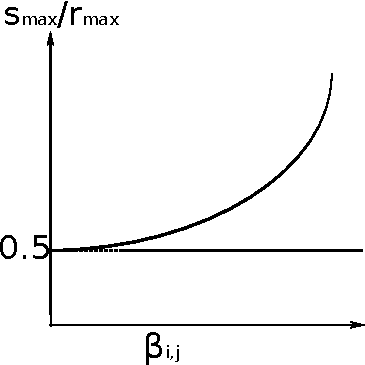
\includegraphics[scale=0.5]{figures/figure15-a}
\par\end{centering}
}\subfigure[\label{fig15-b}]{\begin{centering}
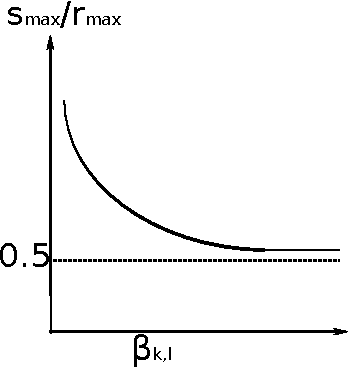
\includegraphics[scale=0.5]{figures/figure15-b}
\par\end{centering}
}
\par\end{centering}
\centering{}\caption{\label{fig15} Change of $s_{max}/r_{max}$: a) $\frac{s_{max}}{r_{max}}$
versus $\beta_{i,j}$ and b) $\frac{s_{max}}{r_{max}}$ versus $\beta_{k,l}$}
\end{figure}


%%BR: Skipped editing from here......
\begin{comment}
\subsection{FMLP \& OMLP versus ECM and RCM
}

\begin{clm}
For ECM's schedulability to be better or equal to that of FMLP or OMLP, 
$s_{max}/|s\_\theta|_{max}$ (in case of FMLP), where $|s\_\theta|_{max}$ be the maximum short request by any task, and $s_{max}/L_{max}$ (in case of OMLP) must  not exceed $O(\frac{m}{n})$, where $L_{max}=max_{\forall i,\forall k}L_{i,k}$. For RCM's schedulability  
to be better or equal  
to that of OMLP, $s_{max}/L_{max}$ must not exceed $O(\frac{m}{n})$.
\end{clm}
\begin{proof}\normalfont
As FMLP is used with G-EDF (GSN-EDF), we compare only ECM 
against it. 
%%BR: "...we compare only ECM against it."??? 
First, we derive upper bounds for the blocking parameters of FMLP. When requests are non-nested, each resource (short or long) will be contained in its own group. Let $N_{i,s}$ be the number of times a task $T_{i}$ requests a short
resource, $|s\_\theta|_{i,max}$ be the maximum request for a
short resource by $T_{i}$, $\alpha_{bw}=N_{i,s}.(m-1)$. Now, FMLP's three  blocking terms, described in Section~\ref{global-fmlp}, are upper bounded as follows:
\begin{eqnarray*}
BW(T_{i}) & \le & \sum_{s\_\theta\in\theta_{i}}(m-1).|s\_\theta|_{i,max}\\
 & = & N_{i,s}.(m-1).|s\_\theta|_{i,max}\\
 & \le & N_{i,s}.(m-1).|s\_\theta|_{max}\\
& = & \alpha_{bw}.|s\_\theta|_{max}
 \end{eqnarray*}
\begin{eqnarray*}
NPB\left(T_{i}\right) & \le & \left(1+N_{i,l}\right).max\left(BW_{k\ne i}\left(T_{k}\right)+|s\_\theta|_{k,max}\right)\\
 & \le & \left(1+N_{i,l}\right).max\left(BW_{k\ne i}\left(T_{k}\right)+|s\_\theta|_{max}\right)\\
 & = & \left(1+N_{i,l}\right).|s\_\theta|_{max}.max_{k\ne i}\left(N_{k,s}.\left(m-1\right)+1\right)\\
 & = & \alpha_{npb}.|s\_\theta|_{max}
 \end{eqnarray*}
 where $\alpha_{npb}=\left(1+N_{i,l}\right).max_{k\ne i}\left(N_{k,s}.\left(m-1\right)+1\right)$.
\begin{eqnarray*}
DB\left(T_{i}\right) & \le & N_{i,l}.\left(n-1\right).|l\_\theta|_{i,max}\\
 & \le & N_{i,l}.\left(n-1\right).|l\_\theta|_{max}\\
 \end{eqnarray*}
If $|l\_\theta|_{max}\le c1.|s\_\theta|_{max}$, where $c1$ is the
minimum constant that satisfies this relation, then
\begin{eqnarray*}
DB\left(T_{i}\right)& \le & N_{i,l}.\left(n-1\right).c1.|s\_\theta|_{max}\\
& = & \alpha_{db}.|s\_\theta|_{max}
\end{eqnarray*}
where $\alpha_{db}=N_{i,l}.\left(n-1\right).c1$. 

The total blocking time of each task is added to the task execution time, and
as before, we compare the total utilization of the G-EDF system (with both contention managers) against that under FMLP. 

Now, for ECM's schedulability to be better than FMLP,
\begin{equation}
 \frac{s_{max}}{|s\_\theta|_{max}}\le
 \frac{\sum_{T_{i}}\left(\alpha_{bw}+\alpha_{npb}+\alpha_{db}\right) \Big/t(T_{i})}{\sum_{T_{i}}\alpha_{edf} \Big/t(T_{i})}
 \label{eq38} \end{equation}

From (\ref{eq38}), it can be seen that $T_{i}$'s blocking time,
under FMLP, depends on $m,\, n$ and the number of times it requests resources
(in contrast to ECM, 
%%BR: "...contrast to ECM,..."???  
under which, $T_i$'s retry cost depends on the number of times a conflicting task $T_{j}$ requests resources). Thus, if $N_{i,s},\, N_{i,l}$, 
and $N_{k,s}$ can all be upper bounded by some constant $C_{2}$,
which is the maximum number of times any task $T_{i}$ can request a short
or long resource, then the numerator in (\ref{eq38}) 
is $O(n(n+m))$, while the denominator is $O(n^{2})$. Therefore:
\begin{equation}
\frac{s_{max}}{|s\_\theta|_{max}}=O\left(\frac{m}{n} \right)
\label{eq45}
\end{equation}
This means that, for $n<m$, the contention between tasks under both STM and
FMLP is low (even for short resources under FMLP), but FMLP is more affected
by $NTB$. When $n>m$, contention increases, but FMLP arranges
requests in a FIFO queue, so it is less affected than ECM, 
%%BR: "..than ECM,...???
which
suffers from conflicting tasks and instances
of each conflicting one. FMLP is not affected by the number of instances
of each conflicting task.

%%%%
Since OMLP's blocking time is bounded by (\ref{eq29}) \[ \therefore 
%\;
bi\le2.\left(m-1\right).L_{max}\sum_{k=1}^{q}N_{i,k}\]
%%BR: THis sentence is awkward. Why don't you say "Let  \[L_{max}=..... Since OMLP's blocking time is ..., \therefore.."


For ECM's schedulability to be better than global OMLP:
\begin{equation}
\frac{s_{max}}{L_{max}}\le\frac{\sum_{T_{i}}\left(2.\left(m-1\right)\sum_{k=1}^{q}N_{i,k}\right) \Big/t\left(T_{i}\right)}{\sum_{T_{i}}\alpha_{edf} \Big/t\left(T_{i}\right)}\label{eq40}\end{equation}

For RCM, the ratio is:
\begin{equation}
\frac{s_{max}}{L_{max}}\le\frac{\sum_{T_{i}}\left(2.\left(m-1\right)\sum_{k=1}^{q}N_{i,k}\right) \Big/t\left(T_{i}\right)}{\sum_{T_{i}}\alpha_{rma} \big/t\left(T_{i}\right)}\label{eq41}\end{equation}


If $\sum_{k=1}^{q}N_{i,k}$ is upper bounded by $C_{3}$, which is
a constant representing the maximum total number of requests for resources
by any task $T_{i}$, then:
\begin{equation}
\frac{s_{max}}{L_{max}}=O\left(\frac{nm}{n^{2}}\right)=O\left(\frac{m}{n}\right)
\label{eq46}
\end{equation}
for each of (\ref{eq40}) and (\ref{eq41}). Claim follows.
\end{proof}
\end{comment}


%%BR: Re-started editing from here:
\section{Conclusions}
\label{sec:ecm-rcm-conclusions}

Under both ECM and RCM,  
a task incurs $2.s_{max}$ retry cost for each of its atomic sections due to a conflict with another task's atomic section. Retries under RCM and lock-free are affected by a larger number of conflicting task instances than under ECM. While task retries under ECM and lock-free are affected by all other tasks, retries under RCM are affected only by higher priority tasks. 


STM and lock-free have similar parameters that affect their retry costs---i.e., the number of conflicting jobs and how many times they access shared objects. The $s_{max}/r_{max}$ ratio determines whether STM is better or as good as lock-free. For ECM, this ratio cannot exceed 1, and it can be 1/2 for higher number of conflicting tasks. For RCM, for the common case, $s_{max}$ must be 1/2 of $r_{max}$, and in some cases, $s_{max}$ can be larger than $r_{max}$ by many orders of magnitude.

%The questions that we ask (see Section~\ref{sec:intro}) are fundamentally analytical in nature, and hence, our results are analytical. However, significant insights can be gained by experimental work on a broad range of embedded software, which is outside our work's scope.
\begin{comment}
Our work raises several questions.  
For example, what are the typical range of values for the different parameters that affect the retry cost (and hence the response time)? How tight is our retry and response time bounds in practice? Can real-time CMs be designed for other multicore real-time schedulers (e.g., partitioned, semi-partitioned), and those that dynamically improve application timeliness behavior? These are important directions for further work. 
\end{comment}

%%%%%%%%%%%%%%%%%%%%%%%%%%%%%%%%

\chapter{\label{ch_lcm}The LCM Contention Manager}
\markright{Mohammed El-Shambakey \hfill Chapter~\ref{ch_lcm}. LCM \hfill}

Under ECM and RCM, each atomic section can be aborted for at most $2.s_{max}$ by a single interfering atomic section. We present a novel contention manager (CM) for resolving transactional conflicts, called length-based CM (or LCM)~\cite{lcmdac2012}. LCM can reduce the abortion time of a single atomic section due to an interfering atomic section below $2.s_{max}$. We upper bound transactional retries and response times under LCM, when used with G-EDF and  G-RMA schedulers. We identify the conditions under which LCM outperforms previous real-time STM CMs and lock-free synchronization.
\begin{comment}
 Our implementation and experimental studies reveal that G-EDF/LCM and G-RMA/LCM have shorter or comparable retry costs and response times than other synchronization techniques.
\end{comment}

The rest of this Chapter is organized as follows: Section~\ref{sec:lcm} presents Length-based Contention Manager (LCM) and illustrates its behaviour. Section~\ref{sec:lcm_properties} derives LCM properties. Response time analysis of tasks under G-EDF/LCM is given in Section~\ref{response g-edf/lcm}. Schedulability of G-EDF/LCM is compared to schedulability of ECM and lock-free in Section~\ref{performance g-edf-lcm}. Section~\ref{rma} gives response time analysis for G-RMA/LCM. Schedulability of G-RMA/LCM is compared against RCM and lock-free in Section~\ref{rma eval}. We conclude Chapter in Section~\ref{sec:conclusions_lcm}.

\section{\label{sec:lcm}Length-based CM}

LCM resolves conflicts based on the priority of conflicting jobs, besides the length of the interfering atomic section, and the length of the interfered atomic section. This is in contrast to ECM and RCM (Chapter~\ref{ecm-rcm}), where conflicts are resolved using the priority of the conflicting jobs. This strategy allows lower priority jobs, under LCM, to retry for lesser time than that under ECM and RCM, but higher priority jobs, sometimes, wait for lower priority ones with bounded priority-inversion.

\subsection{\label{sec 9.1}Design and Rationale}

%Begin algorithm here
\begin{algorithm}
\footnotesize{
\LinesNumbered
\KwData{$s_i^k(\theta)\rightarrow$ interfered atomic section.\\$s_j^l(\theta)\rightarrow$ interfering atomic section.\\$\psi\rightarrow$ predefined threshold $\in [0,1]$.\\$\delta_i^k(\theta)\rightarrow$ remaining execution length of $s_i^k(\theta)$}
\KwResult{which atomic section of $s_i^k(\theta)$ or $s_j^l(\theta)$ aborts}
\eIf{$p_i^k > p_j^l$}
	{$s_j^l(\theta)$ aborts\label{lcm:step_sicommits}\;}
	{$c_{ij}^{kl}=len(s_j^l(\theta))/len(s_i^k(\theta))$\label{step_cijkl}\;
	$\alpha_{ij}^{kl}=ln(\psi)/(ln(\psi)-c_{ij}^{kl})$\label{step_alphaijkl}\;
	$\alpha=\left(len(s_i^k(\theta))-\delta_i^k(\theta)\right)/len(s_i^k(\theta))$\label{step_alpha}\;
	\eIf{$\alpha \le \alpha_{ij}^{kl}$}
	{$s_i^k(\theta)$ aborts\label{lcm:step_siaborts}\;}
	{$s_j^l(\theta)$ aborts\label{step_sjaborts}\;}
	}
	}
\caption{LCM}
\label{alg_lcm}
\end{algorithm}


For both ECM and RCM, $s_{i}^{k}(\theta)$ can be totally repeated if $s_{j}^{l}(\theta)$ --- which belongs to a higher priority job $\tau_{j}^b$ than $\tau_{i}^a$ --- conflicts with $s_{i}^{k}(\theta)$
at the end of its execution, while $s_{i}^{k}(\theta)$ is just about
to commit. Thus, LCM, shown in Algorithm~\ref{alg_lcm}, uses the remaining length of $s_{i}^{k}(\theta)$ when it is interfered,
as well as $len(s_{j}^{l}(\theta))$, to decide which transaction must be aborted. If $p_i^k$ was greater than $p_j^l$, then $s_i^k(\theta)$ would be the one that commits, because it belongs to a higher priority job, and it started before $s_j^l(\theta)$ (step~\ref{lcm:step_sicommits}). Otherwise, $c_{ij}^{kl}$ is calculated (step~\ref{step_cijkl}) to determine whether it is worth aborting $s_i^k(\theta)$ in favor of $s_j^l(\theta)$, because $len(s_j^l(\theta))$ is relatively small compared to the remaining execution length of $s_i^k(\theta)$  (explained further).

We assume that:
\begin{equation}
c_{ij}^{kl}=len(s_{j}^{l}(\theta))/len(s_{i}^{k}(\theta))
\label{cm_eq}\end{equation}
where $c_{ij}^{kl}\in]0,\infty[$, to cover all possible lengths of $s_{j}^{l}(\theta)$.
Our idea is to reduce the opportunity for the abort of $s_{i}^{k}(\theta)$ if it is close to committing when interfered and $len(s_{j}^{l}(\theta))$ is large. This abort opportunity is increasingly reduced as $s_{i}^{k}(\theta)$ gets closer to the end of its execution, or $len(s_{j}^{l}(\theta))$ gets larger. 

On the other hand, as $s_{i}^{k}(\theta)$ is interfered early,
or $len(s_{j}^{l}(\theta))$ is small compared to $s_{i}^{k}(\theta)$'s remaining length, the abort opportunity 
is increased even if $s_i^k (\theta)$ is close to the end of its execution. To decide whether $s_{i}^{k}(\theta)$ must be aborted or not, we use a threshold value $\psi\in[0,1]$ that determines $\alpha_{ij}^{kl}$ (step~\ref{step_alphaijkl}), where $\alpha_{ij}^{kl}$ is the maximum percentage of $len(s_i^k(\theta))$ below which $s_j^l(\theta)$ is allowed to abort $s_i^k(\theta)$. Thus, if the already executed part of $s_i^k(\theta)$ --- when $s_j^l(\theta)$ interferes with $s_i^k(\theta)$ --- does not exceed $\alpha_{ij}^{kl}len(s_i^k(\theta))$, then $s_i^k(\theta)$ is aborted (step~\ref{lcm:step_siaborts}). Otherwise, $s_j^l(\theta)$ is aborted (step~\ref{step_sjaborts}).

%
\begin{figure}[htbp]
\centering
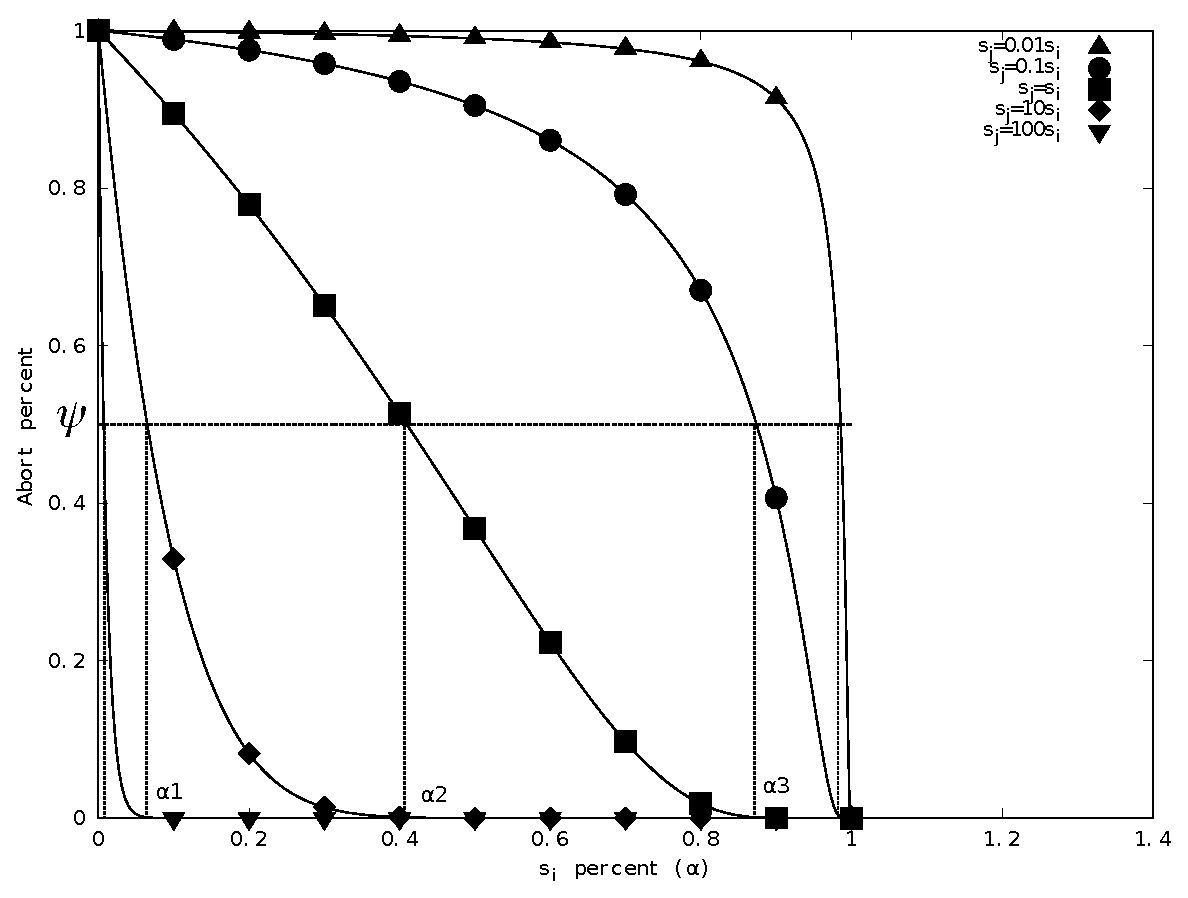
\includegraphics[scale=0.4]{figures/figure16}
\caption{\label{fig16}Interference of $s_{i}^{k}(\theta)$ by various lengths of 
$s_{j}^{l}(\theta)$}
\end{figure}

The behavior of LCM is illustrated in Figure~\ref{fig16}. In this figure, the horizontal axis corresponds to different values of $\alpha$ ranging from $0$ to $1$, and the vertical axis corresponds to different values of abort opportunities, $f(c_{ij}^{kl},\alpha)$, ranging from $0$ to $1$ and calculated by~(\ref{eq49}):
\begin{equation}
f(c_{ij}^{kl},\alpha)=e^{\frac{-c_{ij}^{kl}\alpha}{1-\alpha}}
\label{eq49}\end{equation}
where $c_{ij}^{kl}$ is calculated by~(\ref{cm_eq}).

Figure~\ref{fig16} shows one atomic section $s_i^k(\theta)$ (whose $\alpha$ changes along the horizontal axis) interfered by five different lengths of $s_j^l(\theta)$.
For a predefined value of $f(c_{ij}^{kl},\alpha)$ (denoted as $\psi$ in Algorithm~\ref{alg_lcm}), there corresponds a specific value of $\alpha$ (which is $\alpha_{ij}^{kl}$ in Algorithm~\ref{alg_lcm}) for each curve. For example, when $len(s_j^l(\theta))=0.1 \times len(s_i^k(\theta))$, $s_j^l(\theta)$ aborts $s_i^k(\theta)$ if the latter has not executed more than $\alpha3$ percentage (shown in Figure~\ref{fig16}) of its execution length. As $len(s_{j}^{l}(\theta))$ decreases, the corresponding $\alpha_{ij}^{kl}$ increases (as shown in Figure~\ref{fig16}, $\alpha3>\alpha2>\alpha1$).

Equation (\ref{eq49}) achieves the desired requirement that the abort opportunity is reduced as $s_{i}^{k}(\theta)$ gets
closer to the end of its execution (as $\alpha\rightarrow1,\, f(c_{ij}^{kl},1)\rightarrow0$),
or as the length of the conflicting transaction increases (as $c_{ij}^{kl}\rightarrow\infty,\, f(\infty,\alpha)\rightarrow0$).
Meanwhile, this abort opportunity is increased as $s_{i}^{k}(\theta)$
is interfered closer to its release (as $\alpha\rightarrow0,\, f(c_{ij}^{kl},0)\rightarrow1$),
or as the length of the conflicting transaction decreases (as $c_{ij}^{kl}\rightarrow0,\, f(0,\alpha)\rightarrow1$).

LCM is not a centralized CM, which means that, upon a conflict, each transactions has to decide whether it must commit or abort.

\subsection{LCM Illustrative Example}

Behaviour of LCM can be illustrated by the following example:
\begin{itemize}
\item Transaction $s_{i}^{k}(\theta)\in\tau_{i}^{x}$ begins execution.
Currently, $s_{i}^{k}(\theta)$ does not conflict with any other transaction.
\item Transaction $s_{j}^{l}(\theta)\in\tau_{j}^{y}$ is released while
$s_{i}^{k}(\theta)$ is still running. $p_{j}^{y}>p_{i}^{x}$ (where
priority is dynamic in G-EDF, and fixed in G-RMA). $c_{i,j}^{k,l}$,
$\alpha_{i,j}^{k,l}$ and $\alpha$ are calculated by steps~\ref{step_cijkl} to~\ref{step_alpha} 
in Algorithm~\ref{alg_lcm}. $s_{i}^{k}(\theta)$ has not reached $\alpha$
percentage of its execution length yet. 
\item $\alpha<\alpha_{i,j}^{k,l}$. Then, $s_{j}^{l}(\theta)$ is allowed
to abort and restart $s_{i}^{k}(\theta)$.
\item $s_{j}^{l}(\theta)$ commits. $s_{i}^{k}(\theta)$ executes again.
\item Transaction $s_{h}^{v}(\theta)\in\tau_{h}^{u}$ is released while
$s_{i}^{k}(\theta)$ is running. $p_{h}^{u}>p_{i}^{x}$. $c_{i,h}^{k,v}$,
$\alpha_{i,h}^{k,v}$ and $\alpha$ are calculated by steps~\ref{step_cijkl} to~\ref{step_alpha}
in Algorithm~\ref{alg_lcm}. $s_{i}^{k}(\theta)$ has already passed $\alpha$
percentage of its execution length. So, $s_{h}^{v}(\theta)$ aborts
and restarts in favour of $s_{i}^{k}(\theta)$.
\item Transaction $s_{a}^{b}(\theta)\in\tau_{a}^{f}$ is released. $p_{a}^{f}>p_{i}^{x}$
but $p_{a}^{f}<p_{h}^{u}$. $c_{i,a}^{k,b}$, $\alpha_{i,a}^{k,b}$
and $\alpha$ are calculated by steps~\ref{step_cijkl} to~\ref{step_alpha} in Algorithm~\ref{alg_lcm}.
$s_{i}^{k}(\theta)$ has not reached $\alpha$ percentage of its execution
length yet. So, $s_{a}^{b}(\theta)$ is allowed to abort $s_{i}^{k}(\theta)$.
Because $s_{a}^{b}(\theta)$ is just starting, LCM allows $s_{h}^{v}(\theta)$
to abort $s_{a}^{b}(\theta)$. So, the highest priority transaction
is not blocked by an intermediate priority transaction $s_{a}^{b}(\theta)$.
\item When $s_{h}^{v}(\theta)$ commits. $s_{a}^{b}(\theta)$ is allowed
to execute while $s_{i}^{k}(\theta)$ is retrying.
\item When $s_{a}^{b}(\theta)$ commits, $s_{i}^{k}(\theta)$ executes.
\item Transaction $s_{c}^{n}(\theta)\in\tau_{o}^{z}$ is released while
$s_{i}^{k}(\theta)$ is running. $p_{o}^{z}<p_{i}^{x}$. So, $s_{i}^{k}(\theta)$
commits first, then $s_{c}^{n}(\theta)$ is allowed to proceed.
\end{itemize} 

\section{Properties}\label{sec:lcm_properties}

LCM properties are given by the following Lemmas. These properties are used to derive retry cost and response time of transactions and tasks under LCM.

\begin{clm}
\label{LCM_higher_rc}
Let $s_{j}^{l}(\theta)$ interfere once with $s_{i}^{k}(\theta)$ at $\alpha_{ij}^{kl}$. Then, the maximum contribution of $s_{j}^{l}(\theta)$ to 
$s_{i}^{k}(\theta)$'s 
retry cost is:
\begin{equation}
W_i^k(s_j^l(\theta))\le \alpha_{ij}^{kl}len\Big(s_{i}^{k}(\theta)\Big)+len\Big(s_{j}^{l}(\theta)\Big)\label{eq47}\end{equation}
\end{clm}

\begin{proof}\normalfont
If $s_{j}^{l}(\theta)$ interferes with $s_{i}^{k}(\theta)$
at a $\Upsilon$ percentage, where $\Upsilon<\alpha_{ij}^{kl}$,
then the retry cost of $s_{i}^{k}(\theta)$ is $\Upsilon len(s_{i}^{k}(\theta))+len(s_{j}^{l}(\theta))$, which is lower than that calculated in (\ref{eq47}). Besides, 
if $s_{j}^{l}(\theta)$ interferes with $s_{i}^{k}(\theta)$ after
$\alpha_{ij}^{kl}$ percentage, then $s_{i}^{k}(\theta)$ will not
abort.
\end{proof}


\begin{clm}
\label{LCM_lower_rc}
An atomic section of a higher priority job, $\tau_{j}^b$, may have to abort and retry due to a lower priority job, $\tau_{i}^a$, if $s_{j}^{l}(\theta)$ interferes
with $s_{i}^{k}(\theta)$ after the $\alpha_{ij}^{kl}$ percentage. $\tau_{j}$'s retry time, due to $s_{i}^{k}(\theta)$ and $s_{j}^{l}(\theta)$,
is upper bounded by:
 \begin{equation}
W_j^l(s_i^k(\theta))\le \Big(1-\alpha_{ij}^{kl}\Big)len\Big(s_{i}^{k}(\theta)\Big)\label{eq48}\end{equation}
\end{clm}

\begin{proof}\normalfont
It is derived directly from Claim~\ref{LCM_higher_rc}, as $s_j^l(\theta)$ will have to retry for the remaining length of $s_i^k(\theta)$.
\end{proof}

%sh-start
\begin{clm}
\label{no priority inversion in lcm}
A higher priority job, $\tau_i^z$, suffers from priority inversion for at most number of atomic sections in $\tau_i^z$.
\end{clm}

\begin{proof}\normalfont
Assuming three atomic sections, $s_i^k(\theta)$, $s_j^l(\theta)$ and $s_a^b(\theta)$, where $p_j > p_i$ and $s_j^l(\theta)$ interferes with $s_i^k(\theta)$ after $\alpha_{ij}^{kl}$. Then $s_j^l(\theta)$ will have to abort and retry. At this time, if $s_a^b(\theta)$ interferes with the other two atomic sections, and the LCM decides which transaction to commit based on comparison between each two transactions. So, we have the following cases:-
\begin{itemize}
\item $p_a < p_i < p_j$, then $s_a^b(\theta)$ will not abort any one because it is still in its beginning and it is of the lowest priority. So. $\tau_j$ is not indirectly blocked by $\tau_a$.
\item $p_i<p_a<p_j$ and even if $s_a^b(\theta)$ interferes with $s_i^k(\theta)$ before $\alpha_{ia}^{kb}$, so, $s_a^b(\theta)$ is allowed abort $s_i^k(\theta)$. Comparison between $s_j^l(\theta)$ and $s_a^b(\theta)$ will result in LCM choosing $s_j^l(\theta)$ to commit and abort $s_a^b(\theta)$ because the latter is still beginning, and $\tau_j$ is of higher priority. If $s_a^b(\theta)$ is not allowed to abort $s_i^k(\theta)$, the situation is still the same, because $s_j^l(\theta)$ was already retrying until $s_i^k(\theta)$ finishes.
\item $p_a>p_j>p_i$, then if $s_a^b(\theta)$ is chosen to commit, this is not priority inversion for $\tau_j$ because $\tau_a$ is of higher priority.
\item if $\tau_a$ preempts $\tau_i$, then LCM will compare only between $s_j^l(\theta)$ and $s_a^b(\theta)$. If $p_a<p_j$, then $s_j^l(\theta)$ will commit because of its task's higher priority and $s_a^b(\theta)$ is still at its beginning, otherwise, $s_j^l(\theta)$ will retry, but this will not be priority inversion because $\tau_a$ is already of higher priority than $\tau_j$. If $\tau_a$ does not access any object but it preempts $\tau_i$, then CM will choose $s_j^l(\theta)$ to commit as only already running transactions are competing together.
\end{itemize}
So, by generalizing these cases to any number of conflicting jobs, it is seen that when an atomic section, $s_j^l(\theta)$, of a higher priority job is in conflict with a number of atomic sections belonging to lower priority jobs, $s_j^l(\theta)$ can suffer from priority inversion by only one of them. So, each higher priority job can suffer priority inversion at most its number of atomic section. Claim follows.
\end{proof}

\begin{clm}
\label{max_pri_inv}
The maximum delay suffered by $s_j^l(\theta)$ due to lower priority jobs is caused by the maximum length atomic section accessing object $\theta$, which belongs to a lower priority job than $\tau_j^b$ that owns $s_j^l(\theta)$.
\end{clm}

\begin{proof}\normalfont
Assume three atomic sections, $s_i^k(\theta)$, $s_j^l(\theta)$, and $s_h^z(\theta)$, where $p_j>p_i$, $p_j>p_h$, and $len(s_i^k(\theta))>len(s_h^z(\theta))$. Now, $\alpha_{ij}^{kl}>\alpha_{hj}^{zl}$ and $c_{ij}^{kl}<c_{hj}^{zl}$. By applying~(\ref{eq48}) to obtain the contribution of $s_i^k(\theta)$ and $s_h^z(\theta)$ to the priority inversion of $s_j^l(\theta)$ and dividing them, we get:
\begin{eqnarray*}
\frac{W_{j}^{l}(s_{i}^{k}(\theta))}{W_{j}^{l}(s_{h}^{z}(\theta))} & = & \frac{\left(1-\alpha_{ij}^{kl}\right)len(s_{i}^{k}(\theta))}{\left(1-\alpha_{hj}^{zl}\right)len(s_{h}^{z}(\theta))}
\end{eqnarray*}
By substitution for $\alpha$s from~(\ref{eq49}):
\begin{eqnarray*}
 & = & \frac{(1-\frac{ln\psi}{ln\psi-c_{ij}^{kl}})len(s_{i}^{k}(\theta))}{(1-\frac{ln\psi}{ln\psi-c_{hj}^{zl}})len(s_{h}^{z}(\theta))}
  =  \frac{(\frac{-c_{ij}^{kl}}{ln\psi-c_{ij}^{kl}})len(s_{i}^{k}(\theta))}{(\frac{-c_{hj}^{zl}}{ln\psi-c_{hj}^{zl}})len(s_{h}^{z}(\theta))}\end{eqnarray*}
$\because ln\psi \le 0$ and $c_{ij}^{kl},c_{hj}^{kl} > 0, \therefore$ by substitution from~(\ref{cm_eq})
\begin{eqnarray*}
 & = & \frac{len(s_{j}^{l}(\theta))/(ln\psi-c_{ij}^{kl})}{len(s_{j}^{l}(\theta))/(ln\psi-c_{hj}^{zl})}
  =  \frac{ln\psi-c_{hj}^{zl}}{ln\psi-c_{ij}^{kl}}>1\end{eqnarray*}
Thus, as the length of the interfered atomic section increases, the delay suffered by the interfering atomic section increases. Claim follows.
\end{proof}


\section{\label{response g-edf/lcm}Response Time of G-EDF/LCM}

%Toward establishing the response time under G-EDF/LCM, we introduce a set of Claims.

\begin{clm}\label{GEDF/LCM response time}
$RC(T_i)$ for a task $\tau_i$ under G-EDF/LCM is upper bounded by:

\begin{eqnarray}
RC(T_i) & = & \Bigg(\sum_{\forall \tau_h \in \gamma_i}\sum_{\forall\theta \in \theta_i \wedge \theta_h}\Bigg(\left\lceil\frac{T_{i}}{T_{h}}\right\rceil\sum_{\forall s_{h}^{l}(\theta)}len\Big(s_{h}^{l}(\theta)\Big)\nonumber\\
& + & \alpha_{max}^{hl}len\Big(s_{max}^{h}(\theta)\Big)\Bigg)\Bigg) + \sum_{\forall s_{i}^{y}(\theta)}\left(1-\alpha_{max}^{iy}\right)len\left(s_{max}^i(\theta)\right)  
\label{eq78}\end{eqnarray}

where $\alpha_{max}^{hl}$ is the $\alpha$ value that corresponds to $\psi$ due to the interference of $s_{max}^h(\theta)$ by $s_h^l(\theta)$. $\alpha_{max}^{iy}$ is the $\alpha$ value that corresponds to $\psi$ due to the interference of $s_{max}^i(\theta)$ by $s_i^y(\theta)$.
\end{clm}

\begin{proof}\normalfont
The maximum number of higher priority instances of $\tau_h$ that can interfere with $\tau_i^x$ is $\left\lceil\frac{T_i}{T_h}\right\rceil$, as shown in Figure~\ref{fig17}, where one instance of $\tau_h$ and $\tau_h^p$ coincides with the absolute deadline of $\tau_i^x$.

By using Claims~\ref{gedf-edf},~\ref{LCM_higher_rc},~\ref{LCM_lower_rc},~\ref{no priority inversion in lcm} and~\ref{max_pri_inv} to determine the effect of atomic sections belonging to higher and lower priority instances of interfering tasks to $\tau_i^x$, Claim follows.
\end{proof}


Response time of $\tau_{i}$ is calculated by~(\ref{eq10}).
\begin{figure}
\begin{centering}
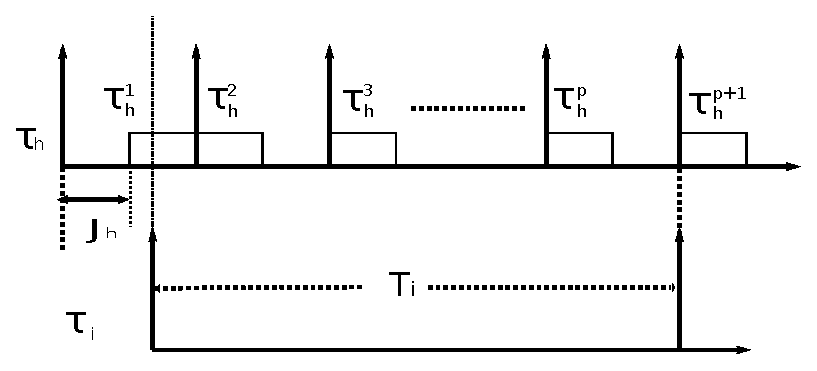
\includegraphics[scale=0.6]{figures/figure18}
\par\end{centering}
\caption{\label{fig17}$\tau_h^p$ has a higher priority than $\tau_i^x$}
\end{figure}

\section{Schedulability of G-EDF/LCM}
\label{performance g-edf-lcm}
We now compare the schedulability of G-EDF/LCM with ECM (Chapter~\ref{ecm-rcm}) to understand when G-EDF/LCM will perform better. 
Toward this, we compare the total utilization of ECM with that of G-EDF/LCM. For each method, we inflate the $c_i$ of each task $\tau_i$ by adding the retry cost suffered by $\tau_i$. Thus, if method $A$ adds retry cost $RC_A(T_i)$ to $c_i$, and method $B$ adds retry cost $RC_B(T_i)$ to $c_i$, then the schedulability of $A$ and $B$ are compared as:
\begin{eqnarray}
\sum_{\forall \tau_{i}}\frac{c_{i}+RC_A(T_{i})}{T_{i}} & \le & \sum_{\forall \tau_{i}}\frac{c_{i}+RC_B(T_{i})}{T_{i}}\nonumber\\
\sum_{\forall \tau_{i}}\frac{RC_A(T_{i})}{T_{i}} & \le & \sum_{\forall \tau_{i}}\frac{RC_B(T_{i})}{T_{i}}
\label{eqa}\end{eqnarray}
Thus, schedulability is compared by substituting the retry cost added by the synchronization methods in (\ref{eqa}).

\subsection{Schedulability of G-EDF/LCM and ECM}
\begin{clm}\label{lcm versus ecm}
Let $s_{max}$ be the maximum length atomic section accessing any object $\theta$. Let $\alpha_{max}$ and $\alpha_{min}$ be the maximum and minimum values of $\alpha$ for any two atomic sections $s_i^k(\theta)$ and $s_j^l(\theta)$. Given a threshold $\psi$, schedulability of G-EDF/LCM is equal or better than ECM if for any task $\tau_i$:
\begin{equation}
\frac{1-\alpha_{min}}{1-\alpha_{max}} \le \sum_{\forall \tau_h \in \gamma_i}\left\lceil\frac{T_i}{T_h}\right\rceil
\label{edf-lcm-ecm}\end{equation}
\end{clm}

\begin{proof}\normalfont
Under ECM, $RC(T_{i})$ is upper bounded by:
\begin{equation}
RC(T_{i})\le\sum_{\forall \tau_{h}\in\gamma_{i}}\sum_{\forall \theta\in\ (\theta_{i}\wedge\theta_{h})}\left(\left\lceil\frac{T_{i}}{T_{h}}\right\rceil\sum_{\forall s_{h}^{z}(\theta)}2len(s_{max})\right)\label{eq61}\end{equation}
with the assumption that all lengths of atomic sections of (\ref{eq3}), (\ref{eq4}) and~(\ref{eq78}) are replaced by $s_{max}$.
%~\cite{stmconcurrencycontrol:emsoft11}. 
Let $\alpha_{max}^{hl}$ in~(\ref{eq78}) be replaced with $\alpha_{max}$, and $\alpha_{max}^{iy}$ in~(\ref{eq78}) be replaced with $\alpha_{min}$. 
As $\alpha_{max}$, $\alpha_{min}$, and $len(s_{max})$ are all constants, (\ref{eq78}) is upper bounded by:
\begin{eqnarray}
RC(T_i) & \le & \Bigg(\sum_{\forall \tau_h \in \gamma_i}\sum_{\forall\theta \in \theta_i \wedge \theta_h}\Bigg(\left\lceil\frac{T_{i}}{T_{h}}\right\rceil\sum_{\forall s_{h}^{l}(\theta)}\left(1+\alpha_{max}\right)\nonumber\\
& & len\Big(s_{max}\Big)\Bigg)\Bigg)
 +  \sum_{\forall s_{i}^{y}(\theta)}\Big(1-\alpha_{min}\Big)len\Big(s_{max}\Big)\nonumber\\ 
\label{eq101}\end{eqnarray}

If $\beta_1^{ih}$ is the total number of times any instance of $\tau_h$ accesses shared objects with $\tau_i$, then $\beta_1^{ih}=\sum_{\forall \theta\in(\theta_{i}\wedge\theta_{h})}\sum_{\forall s_{h}^{z}(\theta)}$. Furthermore, if $\beta_2^i$ is the total number of times any instance of $\tau_i$ accesses shared objects with any other instance,   $\beta_2^i=\sum_{\forall s_{i}^{y}(\theta)}$\textit{, where $\theta$ is shared with another task}. Then, $\beta_{i}=max\{max_{\forall \tau_h \in \gamma_i}\{\beta_1^{ih}\},\beta_2^i\}$ is the maximum number of accesses to all shared objects by any instance of $\tau_{i}$ or $\tau_{h}$. 
Thus, (\ref{eq61}) becomes:
\begin{equation}
RC(T_{i})\le\sum_{\tau_{h}\in\gamma_{i}}2\left\lceil\frac{T_{i}}{T_{h}}\right\rceil\beta_{i}len(s_{max})
\label{eq63}\end{equation}
and (\ref{eq101}) becomes:
%\begin{eqnarray}
%RC(T_{i}) & \le & \beta_{i}len(s_{max}) \Bigg((1-\alpha_{min})\nonumber\\
%& + & \sum_{\forall \tau_h \in \gamma_i}\left\lceil\frac{T_{i}}{T_{h}}\right\rceil(1+\alpha_{max})\Bigg)
%\label{eq102}\end{eqnarray}

\begin{equation}
RC(T_{i}) \le \beta_{i}len(s_{max}) \left((1-\alpha_{min}) + \sum_{\forall \tau_h \in \gamma_i}\left\lceil\frac{T_{i}}{T_{h}}\right\rceil(1+\alpha_{max})\right)
\label{eq102}\end{equation}

We can now compare the total utilization of G-EDF/LCM with that of ECM by comparing~(\ref{eq101}) and~(\ref{eq102}) for all $\tau_i$:
\begin{eqnarray}
& & \sum_{\forall \tau_{i}}\frac{(1-\alpha_{min})+\sum_{\forall \tau_{h}\in\gamma_{i}}\left(\left\lceil\frac{T_{i}}{T_{h}}\right\rceil(1+\alpha_{max})\right)}{T_{i}} \nonumber\\
& \le &   \sum_{\forall \tau_{i}}\frac{\sum_{\forall \tau_{h}\in\gamma_{i}}2\left\lceil\frac{T_{i}}{T_{h}}\right\rceil}{T_{i}}\label{eqc}\end{eqnarray}

(\ref{eqc}) is satisfied if for each $\tau_{i}$, the following condition is satisfied:
\begin{equation*}
(1-\alpha_{min})+\sum_{\forall \tau_h \in \gamma_i}\left(\left\lceil\frac{T_{i}}{T_{h}}\right\rceil(1+\alpha_{max})\right)  \le  2\sum_{\forall \tau_h \in \gamma_i}\left\lceil\frac{T_{i}}{T_{h}}\right\rceil
\end{equation*}
\begin{equation*}
\therefore\frac{1-\alpha_{min}}{1-\alpha_{max}}  \le  \sum_{\forall \tau_h \in \gamma_i}\left\lceil\frac{T_{i}}{T_{h}}\right\rceil
\end{equation*}
Claim follows.
\end{proof}


\subsection{G-EDF/LCM versus Lock-free}
\label{gedf-lcm-lock-free}
We consider the retry-loop lock-free synchronization for G-EDF given in~\cite{key-5}. This lock-free approach is the most relevant to our work. 

\begin{clm}\label{gedf-lcm-lock-free_clm} 
Let $s_{max}$ denote $len(s_{max})$ and $r_{max}$ denote the maximum execution cost of a single iteration of any retry loop of any task in the retry-loop lock-free algorithm in~\cite{key-5}. Now, G-EDF/LCM achieves higher schedulability than the retry-loop lock-free approach if the upper bound on $s_{max}/r_{max}$ under G-EDF/LCM ranges between 0.5 and 2 (which is higher than that under  ECM). 
\end{clm}

\begin{proof}\normalfont
From~\cite{key-5}, the retry-loop lock-free algorithm
is upper bounded by: 
\begin{equation}
RL(T_{i})=\sum_{\tau_{h}\in\gamma_{i}}\left(\left\lceil \frac{T_{i}}{T_{h}}\right\rceil +1\right)\beta_{i}r_{max}\label{eq32-1}
\end{equation}
 where $\beta_{i}$ is as defined in Claim~\ref{lcm versus ecm}.
The retry cost of $\tau_{i}$ in G-EDF/LCM is upper bounded by (\ref{eq102}).
By comparing G-EDF/LCM's total utilization with that of the retry-loop
lock-free algorithm, we get: 
\begin{eqnarray*}
 & \sum_{\forall\tau_{i}}\frac{\left((1-\alpha_{min})+\sum_{\forall\tau_{h}\in\gamma_{i}}\left(\left\lceil \frac{T_{i}}{T_{h}}\right\rceil (1+\alpha_{max})\right)\right)\beta_{i}s_{max}}{T_{i}}\\
\le & \sum_{\forall\tau_{i}}\frac{\sum_{\forall\tau_{h}\in\gamma_{i}}\left(\left\lceil \frac{T_{i}}{T_{h}}\right\rceil +1\right)\beta_{i}r_{max}}{T_{i}}
\end{eqnarray*}
 
\begin{eqnarray}
\therefore\frac{s_{max}}{r_{max}}\le\frac{\sum_{\forall\tau_{i}}\frac{\sum_{\forall\tau_{h}\in\gamma_{i}}\left(\left\lceil \frac{T_{i}}{T_{h}}\right\rceil +1\right)\beta_{i}}{T_{i}}}{\sum_{\forall\tau_{i}}\frac{\left((1-\alpha_{min})+\sum_{\forall\tau_{h}\in\gamma_{i}}\left(\left\lceil \frac{T_{i}}{T_{h}}\right\rceil (1+\alpha_{max})\right)\right)\beta_{i}}{T_{i}}}\label{u-gedf-lcm-ecm}
\end{eqnarray}


Let the number of tasks that have shared objects with $\tau_{i}$
be $\omega$ (i.e., $\sum_{\tau_{h}\in\gamma_{i}}=\omega\ge1$ since
at least one task has a shared object with $\tau_{i}$; otherwise,
there is no conflict between tasks). Let the total number of tasks
be $n$, so $1\le\omega\le n-1$, and $\left\lceil \frac{T_{i}}{T_{h}}\right\rceil \in[1,\infty[$.
To find the minimum and maximum values for the upper bound on $s_{max}/r_{max}$,
we consider the following cases: 
\begin{itemize}
\item $\alpha_{min}\rightarrow0,\alpha_{max}\rightarrow0$ 
\end{itemize}
$\therefore$~(\ref{u-gedf-lcm-ecm}) will be: 
\begin{eqnarray}
\frac{s_{max}}{r_{max}} & \le & 1+\frac{\sum_{\forall\tau_{i}}\frac{\omega-1}{T_{i}}}{\sum_{\forall\tau_{i}}\frac{1+\sum_{\forall\tau_{h}\in\gamma_{i}}\left\lceil \frac{T_{i}}{T_{h}}\right\rceil }{T_{i}}}\nonumber \\
\label{s-r-1}
\end{eqnarray}
 By substituting the edge values for $\omega$ and $\left\lceil \frac{T_{i}}{T_{h}}\right\rceil $
in~(\ref{s-r-1}), we derive that the upper bound on $s_{max}/r_{max}$
lies between 1 and 2.
\begin{itemize}
\item $\alpha_{min}\rightarrow0,\alpha_{max}\rightarrow1$ 
\end{itemize}
(\ref{u-gedf-lcm-ecm}) becomes 
\begin{eqnarray}
\frac{s_{max}}{r_{max}} & \le & 0.5+\frac{\sum_{\forall\tau_{i}}\frac{\omega-0.5}{T_{i}}}{\sum_{\forall\tau_{i}}\frac{1+2\sum_{\forall\tau_{h}\in\gamma_{i}}\left\lceil \frac{T_{i}}{T_{h}}\right\rceil }{T_{i}}}\label{s-r-2}
\end{eqnarray}
 By applying the edge values for $\omega$ and $\left\lceil \frac{T_{i}}{T_{h}}\right\rceil $
in~(\ref{s-r-2}), we derive that the upper bound on $s_{max}/r_{max}$
lies between 0.5 and 1.
\begin{itemize}
\item $\alpha_{min}\rightarrow1,\alpha_{max}\rightarrow0$ 
\end{itemize}
This case is rejected since $\alpha_{min}\le\alpha_{max}$.
\begin{itemize}
\item $\alpha_{min}\rightarrow1,\alpha_{max}\rightarrow1$ 
\end{itemize}
$\therefore$~(\ref{u-gedf-lcm-ecm}) becomes: 
\begin{eqnarray}
\frac{s_{max}}{r_{max}} & \le & 0.5+\frac{\sum_{\tau_{i}}\frac{\omega}{T_{i}}}{2\sum_{\tau_{i}}\frac{\sum_{\forall\tau_{h}\in\gamma_{i}}\left\lceil \frac{T_{i}}{T_{h}}\right\rceil }{T_{i}}}\label{s-r-4}
\end{eqnarray}
 By applying the edge values for $\omega$ and $\left\lceil \frac{T_{i}}{T_{h}}\right\rceil $
in~(\ref{s-r-4}), we derive that the upper bound on $s_{max}/r_{max}$
lies between 0.5 and 1, which is similar to that achieved by ECM.

Summarizing from the previous cases, the upper bound on $s_{max}/r_{max}$
lies between 0.5 and 2, whereas for ECM,
it lies between 0.5 and 1. Claim follows.

\end{proof}

\section{Response Time of G-RMA/LCM}
\label{rma}

\begin{clm}\label{response g-rma/lcm}
Let $\lambda_{2}(j,\theta)=\sum_{\forall s_{j}^{l}(\theta)}len(s_{j}^{l}(\theta))+\alpha_{max}^{jl}len(s_{max}^{j}(\theta))$, where $\alpha_{max}^{jl}$ is the $\alpha$ value corresponding to $\psi$ due to the interference of $s_{max}^j(\theta)$ by $s_j^l(\theta)$. The retry cost of any task $\tau_i$ under G-RMA/LCM during $T_i$ 
is given by:
%\begin{eqnarray}
%RC\left(T_i\right) & = &
%  \sum_{\forall \tau_{j}^{*}}\left(\sum_{\theta\in(\theta_{i}\wedge\theta_{j})}\left(\left(\left\lceil\frac{T_i}{T_{j}}\right\rceil +1\right)\lambda_{2}(j,\theta)\right)\right)\nonumber\\
%& + & \sum_{\forall s_{i}^{y}(\theta)}\Big(1-\alpha_{max}^{iy}\Big)len\Big(s_{max}^i(\theta)\Big)
%\label{eq60}
%\end{eqnarray}
\begin{equation}
RC\left(T_i\right) = \sum_{\forall\tau_{j}^{*}}\left(\sum_{\theta\in(\theta_{i}\wedge\theta_{j})}\left(\left(\left\lceil\frac{T_i}{T_{j}}\right\rceil +1\right)\lambda_{2}(j,\theta)\right)\right) + \sum_{\forall s_{i}^{y}(\theta)}\left(1-\alpha_{max}^{iy}\right)len\left(s_{max}^i(\theta)\right)
\label{eq60}
\end{equation}

where $\tau_{j}^{*}=\{\tau_{j}|(\tau_{j}\in\gamma_{i})\wedge(p_{j}>p_{i})\}$.
\end{clm}

\begin{proof}\normalfont
Under G-RMA, all instances of a higher priority task, $\tau_{j}$, can conflict with a lower priority task,
$\tau_{i}$, during $T_{i}$. (\ref{eq47}) can be used to determine the contribution of each conflicting atomic section in $\tau_j$ to $\tau_i$. Meanwhile, all instances of any task with lower priority than $\tau_{i}$ can conflict with $\tau_i$ during $T_{i}$. Claims~\ref{LCM_lower_rc} and~\ref{no priority inversion in lcm} can be used to determine the contribution of conflicting atomic sections in lower priority tasks to $\tau_i$.
%
  %over the whole $t(T_i)$ (unlike the case of G-EDF/LCM, where (\ref{eq59}) chooses which equation to use depending on whether or not $L$ is less than $\left\lfloor\frac{t(T_{i})-c_{h}}{t(T_{h})}\right\rfloor t(T_{h})+c_{h}$).
Using the previous notations and Claim~\ref{clm:rcm_retry_cost}, the Claim follows.
\end{proof}

The response time is calculated by~(\ref{eq22}) with replacing $RC(R_i^{up})$ with $RC(T_i)$.
%BR: You should say "..with $RC(T_i)$ replacing $RC(R_i^{up})$."

\section{Schedulability of G-RMA/LCM}
\label{rma eval}

\subsection{Schedulability of G-RMA/LCM and RCM}

\begin{clm}\label{rma_eval_clm}
Under the same assumptions of Claims~\ref{lcm versus ecm} and~\ref{response g-rma/lcm}, G-RMA/LCM's schedulability is equal or better than RCM if:
\begin{equation}
\frac{1-\alpha_{min}}{1-\alpha_{max}}\le \sum_{\forall \tau_j^*}\left( \left\lceil\frac{T_i}{T_j}\right\rceil +1 \right)
\label{eq70}\end{equation}
\end{clm}

\begin{proof}\normalfont
Under the same assumptions as that of Claims~\ref{lcm versus ecm} and~\ref{response g-rma/lcm}, (\ref{eq60}) can be upper bounded as:
%\begin{eqnarray}
%RC(T_i) & \le & \sum_{\forall \tau_{j}^{*}}\bigg(\left(\left\lceil\frac{T_{i}}{T_{j}}\right\rceil +1\right)(1+\alpha_{max})
% len(s_{max})\beta_{i}\bigg)\nonumber\\
% & + & (1-\alpha_{min})len(s_{max})\beta_{i}\label{eq68}\end{eqnarray}
\begin{equation}
RC(T_i) \le \sum_{\forall \tau_{j}^{*}}\left(\left(\left\lceil\frac{T_{i}}{T_{j}}\right\rceil +1\right)(1+\alpha_{max}) len(s_{max})\beta_{i}\right) + (1-\alpha_{min})len(s_{max})\beta_{i}\label{eq68}\end{equation} 
 
For RCM, (\ref{eq20}) for $RC(T_{i})$ is upper bounded by:
\begin{equation*}
RC(T_{i})\le\sum_{\forall \tau_{j}^{*}}\left(\left\lceil\frac{T_{i}}{T_{j}}\right\rceil +1\right)2\beta_{i}len(s_{max})\label{eq69}\end{equation*}\
By comparing the total utilization of G-RMA/LCM with that of RCM,
we get:
\begin{eqnarray}
 & \sum_{\forall\tau_{i}}\frac{len\left(s_{max}\right)\beta_{i}\left(\left(1-\alpha_{min}\right)+\sum_{\forall\tau_{j}^{*}}\left(\left(\left\lceil\frac{T_{i}}{T_{j}}\right\rceil+1\right)\left(1+\alpha_{max}\right)\right)\right)}{T_{i}}\nonumber\\
\le & \sum_{\forall\tau_{i}}\frac{2len\left(s_{max}\right)\beta_{i}\sum_{\forall\tau_{j}^{*}}\left(\left\lceil\frac{T_{i}}{T_{j}}\right\rceil+1\right)}{T_{i}}\label{grma-lcm-rcm}\end{eqnarray}
(\ref{grma-lcm-rcm}) is satisfied if $\forall \tau_i$~(\ref{eq70}) is satisfied. Claim follows.
\end{proof}


\subsection{G-RMA/LCM versus Lock-free}\label{g-rma lcm vs lock-free}

Although~\cite{key-5} considers retry-loop lock-free synchronization
for G-EDF systems,~\cite{key-5} also applies for G-RMA systems.

\begin{clm}\label{lcm rma lock-free comparison clm}

Let $s_{max}$ denote $len(s_{max})$ and $r_{max}$ denote the maximum
execution cost of a single iteration of any retry loop of any task
in the retry-loop lock-free algorithm in~\cite{key-5}. G-RMA/LCM
achieves higher schedulability than the retry-loop lock-free approach
if the upper bound on $s_{max}/r_{max}$ under G-RMA/LCM is no less
than 0.5. Upper bound on $s_{max}/r_{max}$ can extend to large values
when $\alpha_{min}$ and $\alpha_{max}$ are very large.

\end{clm}

\begin{proof}\normalfont

The retry cost for G-RMA/LCM is upper bounded by~(\ref{eq60}). Let $\gamma_{i}=\tau_{j}^{*}\cup\bar{\tau_{j}}$,
where $\tau_{j}^{*}$ is the set of higher priority tasks than $\tau_{i}$
sharing objects with $\tau_{i}$. $\bar{\tau_{j}}$ is the set
of lower priority tasks than $\tau_{i}$ sharing objects with
it. We follow the same definitions of $\beta_{i},\, r_{max}$, and
$RL(T_{i})$ given in the proof of Claim (\ref{gedf-lcm-lock-free_clm}).
Schedulability of G-RMA/LCM equals or exceeds the schedulability of retry-loop
lock-free algorithm if:
\begin{eqnarray}
\frac{s_{max}}{r_{max}} & \le & \frac{\sum_{\forall\tau_{i}}\frac{\sum_{\tau_{j}^{*}}\left(\left\lceil \frac{T_{i}}{T_{j}}\right\rceil +1\right)}{T_{i}}}{\sum_{\forall\tau_{i}}\frac{\Big(1-\alpha_{min}\Big)+\sum_{\tau_{j}^{*}}\left(\left\lceil \frac{T_{i}}{T_{j}}\right\rceil +1\right)\left(1+\alpha_{max}\right)}{T_{i}}}\nonumber\\
 & + & \frac{2\sum_{\forall\tau_{i}}\frac{\sum_{\forall\bar{\tau_{j}}}}{T_{i}}}{\sum_{\forall\tau_{i}}\frac{\Big(1-\alpha_{min}\Big)+\sum_{\tau_{j}^{*}}\left(\left\lceil \frac{T_{i}}{T_{j}}\right\rceil +1\right)\left(1+\alpha_{max}\right)}{T_{i}}}\nonumber\\
 & & \label{eq:lcm rma lock-free comparison 1} 
\end{eqnarray}
If $p_{j}<p_{i},\,\therefore\,\left\lceil \frac{T_{i}}{T_{j}}\right\rceil =1$, 
because the system assumes implicit deadline tasks and uses the G-RMA
scheduler. 
%
Let $\omega_{1}$ be the size of $\tau_i^*$ and $\omega_{2}$
be the size of $\bar{\tau_i}$. $\therefore$ $\omega_{1}^{i}\ge 1$ and $\omega_{2}^{i}\ge1$.
Otherwise, there is no conflict with $\tau_{i}$. To find the maximum
and minimum upper bounds for $s_{max}/r_{max}$, the following cases
are considered:
\begin{itemize}
\item $\alpha_{min}\rightarrow0,\,\alpha_{max}\rightarrow0$
\begin{equation}
\therefore\frac{s_{max}}{r_{max}}\le1+\frac{\sum_{\forall\tau_{i}}\frac{2\omega_{2}^{i}-1}{T_{i}}}{\sum_{\forall\tau_{i}}\frac{1+\sum_{\tau_{j}^{*}}\left(\left\lceil \frac{T_{i}}{T_{j}}\right\rceil +1\right)}{T_{i}}}\label{eq:lcm rma lock-free comparison 3}
\end{equation}
As the second term in (\ref{eq:lcm rma lock-free comparison 3}) is
always positive (because $\omega_{2}^{i}\ge1$), the minimum
upper bound on $s_{max}/r_{max}$ is $1$. To get the maximum upper
bound on $s_{max}/r_{max}$, let $\left\lceil \frac{T_{i}}{T_{j}}\right\rceil $
approach its minimum value of $1$, $\omega_{1}^{i}\rightarrow0$, and $\omega_{2}^{i}\rightarrow n-1$ 
(the maximum and minimum values for $\omega_{1}^{i}$ and $\omega_{2}^{i}$, 
respectively. $n$ is number of tasks). Now:
\[
\therefore\frac{s_{max}}{r_{max}}\le\left(2n-2\right)
\]
Of course, $n$ cannot be lower than $2$. Otherwise, there will be
no conflicting tasks.

\item $\alpha_{min}\rightarrow0,\,\alpha_{max}\rightarrow1$
\begin{equation}
\frac{s_{max}}{r_{max}}\le\frac{1}{2}+\frac{\sum_{\forall\tau_{i}}\frac{4\omega_{2}^{i}-1}{T_{i}}}{2\sum_{\forall\tau_{i}}\frac{1+2\sum_{\tau_{j}^{*}}\left(\left\lceil \frac{T_{i}}{T_{j}}\right\rceil +1\right)}{T_{i}}}\label{eq:lcm rma lock-free comparison 4}
\end{equation}
The minimum upper bound for $s_{max}/r_{max}$ is $0.5$. This can
happen when $T_{i}\gg T_{j}$. To get the maximum upper bound on $s_{max}/r_{max}$,
let $\left\lceil \frac{T_{i}}{T_{j}}\right\rceil $ approach its
minimum value $1$, $\omega_{2}^{i}\rightarrow n-1$, and $\omega_{1}^{i}\rightarrow0$. 
Now:
\[
\frac{s_{max}}{r_{max}}\le2n-2
\]

\item $\alpha_{min}\rightarrow1,\,\alpha_{max}\rightarrow0$
This case is rejected because $\alpha_{max}$ must be greater or equal
to $\alpha_{min}$.

\item $\alpha_{min}\rightarrow1,\,\alpha_{max}\rightarrow1$
\begin{equation}
\frac{s_{max}}{r_{max}}\le\frac{1}{2}+\frac{\sum_{\forall\tau_{i}}\frac{\omega_{2}^{i}}{T_{i}}}{\sum_{\forall\tau_{i}}\frac{\sum_{\tau_{j}^{*}}\left(\left\lceil \frac{T_{i}}{T_{j}}\right\rceil +1\right)}{T_{i}}}\label{eq:lcm rma lock-free comparison 5}
\end{equation}
The minimum upper bound for $s_{max}/r_{max}$ is $0.5$. This can
happen when $T_{i}\gg T_{j}$. To get the maximum upper bound on $s_{max}/r_{max}$,
let $\left\lceil \frac{T_{i}}{T_{j}}\right\rceil $ approach its
minimum value $1$, $\omega_{2}^{i}\rightarrow n-1,\,\omega_{1}^{i}\rightarrow0$.
%BR: Again, you may need an "and". 
Now:  
\[
\frac{s_{max}}{r_{max}}\rightarrow\infty
\]

\end{itemize}
From the previous cases, we can derive that the upper bound on $s_{max}/r_{max}$
extends from $0.5$ to large values. Claim follows.
\end{proof}

\section{Conclusions}
\label{sec:conclusions_lcm}

In ECM and RCM, a task incurs at most $2s_{max}$ retry cost for each of its atomic section due to conflict
with another task's atomic section. With LCM, this retry cost is reduced to $(1+\alpha_{max})s_{max}$ for each aborted atomic section. In ECM and RCM, tasks do not retry due to lower priority tasks, whereas in LCM, they do so. In G-EDF/LCM, retry due to a lower priority job is encountered only from a task $\tau_{j}$'s last job instance 
during $\tau_{i}$'s period. This is not the case with G-RMA/LCM, because,  each higher priority task can be aborted and retried by any job instance of lower priority tasks. Schedulability of G-EDF/LCM and G-RMA/LCM is better or equal to ECM and RCM, respectively, by proper choices for $\alpha_{min}$ and $\alpha_{max}$. Schedulability of G-EDF/LCM is better than retry-loop lock-free synchronization for G-EDF if the upper bound on $s_{max}/r_{max}$ is between 0.5 and 2, which is higher than that achieved by ECM. 
G-RMA/LCM achieves higher schedulability than retry-loop lock-free synchronization if $s_{max}/r_{max}$ is not greater than 0.5. For high values of $\alpha$ in G-RMA/LCM, $s_{max}/r_{max}$ can extend to large values.

%%%%%%%%%%%%%%%%%%%%%%%%%%%%%%%%

\chapter{\label{ch_pnf}The PNF Contention Manager}
\markright{Mohammed El-Shambakey \hfill Chapter~\ref{ch_pnf}. PNF \hfill}


In this chapter, we present a novel contention manager for resolving transactional conflicts, called PNF~\cite{pnf_emsoft12}. We upper bound transactional retries and task response times under PNF, when used with the G-EDF and  G-RMA schedulers. We formally identify the conditions under which PNF outperforms previous real-time STM contention managers and lock-free synchronization.
\begin{comment}
 We also implement PNF and competitor techniques in the Rochester STM framework and conduct experimental studies using a real-time Linux kernel to understand average-case performance. Our work reveals that G-EDF/PNF and G-RMA/PNF have shorter or comparable retry costs than other synchronization techniques.
\end{comment}

The rest of this Chapter is organized as follows: Section~\ref{probelm description} discusses limitations of previous contention managers and the motivation to PNF. Section~\ref{PNF} give a formal description of PNF. Section~\ref{pnf properties sec} derives PNF's properties. We upper bound retry cost and response time under PNF in Section~\ref{rc pnf sec}. Schedulability comparison between PNF and previous synchronization techniques is given in Section~\ref{sec:pnf-sched-comparison}. We conclude Chapter in Section~\ref{pnf_conclusion}.


\section{Limitations of ECM, RCM, and LCM}\label{probelm description}

%\begin{comment}
ECM, RCM and LCM~\cite{stmconcurrencycontrol:emsoft11,lcmdac2012} assumes that each transaction accesses only one object. This assumption simplifies the retry cost (Claims~\ref{clm:min_gedf-edf},~\ref{clm:rcm_retry_cost},~\ref{GEDF/LCM response time} and~\ref{response g-rma/lcm}) and response time analysis (Sections~\ref{sec:g-edf-edf-cm},~\ref{sec:g-rma-rma-cm},~\ref{response g-edf/lcm} and~\ref{rma}). Besides, it enables a one-to-one comparison with lock-free synchronization in~\cite{key-5}. With multiple objects per transaction, ECM, RCM and LCM will face transitive retry, which we illustrate with an example.


\textbf{Example 1.} Consider three atomic sections $s_{1}^{x}$, $s_{2}^{y}$, 
and $s_{3}^{z}$ belonging to jobs $\tau_{1}^{x}$,$\tau_{2}^{y}$, 
and $\tau_{3}^{z}$, with priorities $p_{3}^{z}>p_{2}^{y}>p_{1}^{x}$, respectively. 
Assume that $s_{1}^{x}$ and $s_{2}^{y}$ share objects, $s_{2}^{y}$ and $s_{3}^{z}$
share objects. $s_{1}^{x}$ and $s_{3}^{z}$ do not share objects.
$s_{3}^{z}$ can cause $s_{2}^{y}$ to retry, which in turn will cause $s_{1}^{x}$ to retry. 
This means that $s_{1}^{x}$ may retry transitively
because of $s_{3}^{z}$, which will increase the retry cost of $s_{1}^{x}$.

Assume another atomic section $s_4^f$ is introduced. Priority of $s_4^f$ is higher than priority of $s_3^z$. $s_4^f$ shares objects only with $s_3^z$. Thus, $s_4^f$ can make $s_3^z$ to retry, which in turn will make $s_2^y$ to retry, and finally, $s_1^x$ to retry. Thus, transitive retry will move from $s_{4}^{f}$ to $s_{1}^{x}$, increasing the retry cost of $s_{1}^{x}$. 
The situation gets worse as more tasks of higher priorities are added, where each task
shares objects with its immediate lower priority task. $\tau_{3}^{z}$
may have atomic sections that share objects with $\tau_{1}^{x}$,
but this will not prevent the effect of transitive retry due to $s_{1}^{x}$.

\begin{mydef}
\textbf{Transitive Retry:} A transaction $s_{i}^{k}$ suffers from
transitive retry when it conflicts with a higher priority transaction
$s_{j}^{l}$, which in turn conflicts with a higher priority transaction
$s_{z}^{h}$, but $s_{i}^{k}$ does not conflict with $s_{z}^{h}$.
Still, when $s_{j}^{l}$ retries due to $s_{z}^{h}$, $s_{i}^{k}$
also retries due to $s_{j}^{l}$. Thus, the effect of the higher priority
transaction $s_{z}^{h}$ is transitively moved to the lower priority
transaction $s_{i}^{k}$, even when they do not conflict on common objects.
\end{mydef}

\begin{clm}\label{ecm-rcm-transitive-retry}
ECM, RCM and LCM suffer from transitive retry for multi-object transactions.
\end{clm}
\begin{proof}\normalfont
ECM, RCM and LCM depend on priorities to resolve conflicts between transactions. Thus, lower priority transaction must always be aborted for a conflicting higher priority transaction in ECM and RCM. In LCM, lower priority transactions are conditionally aborted for higher priority ones. Claim follows. 
\end{proof}

Therefore, the analysis in Chapters~\ref{ecm-rcm} and~\ref{ch_lcm} must extend the set of objects that can cause an atomic section of a lower priority job to retry.  This can be done by initializing the set of conflicting objects, $\gamma_i$, to all objects accessed by all transactions of $\tau_i$. We then cycle through all transactions belonging to all other higher priority tasks. Each transaction $s_j^l$ that accesses at least one of the objects in $\gamma_i$ adds all other objects accessed by $s_j^l$ to $\gamma_i$. The loop over all higher priority tasks is repeated, each time with the new $\gamma_i$, until there are no more transactions accessing any object in $\gamma_i$\footnote{However, note that, this solution may over-extend the set of conflicting objects, and may even contain all objects accessed by all tasks.}.

In addition to the \emph{transitive retry} problem, retrying higher priority transactions can prevent lower priority tasks from running. This happens when all processors are busy with higher priority jobs. When a transaction retries, the processor time is wasted. Thus, it would be better to give the processor to some other task.


Essentially, what we present is a new contention manager that avoids the effect of transitive retry. We call it, Priority contention manager with Negative values and First access (or PNF). PNF also tries to enhance processor utilization. This is done by allocating processors to jobs with non-retrying transactions. PNF is described in Section \ref{PNF}.

\section{The PNF Contention Manager\label{PNF}}

Algorithm \ref{PNF-algorithm} describes PNF. It
manages two sets. The first is the $m$-set, which contains at most $m$ non-conflicting
transactions, where $m$ is the number of processors, as
there cannot be more than $m$ executing transactions (or generally,
$m$ executing jobs) at the same time. When a transaction is entered
in the $m$-set, it executes non-preemptively and no other transaction
can abort it. A transaction in the $m$-set is called an \emph{executing
transaction}. 
This means that, when a transaction is executing before
the arrival of higher priority conflicting transactions, then the
one that started executing first will be committed (Step~\ref{s_i^k commit}). 
%(hence the word ``First'' in the algorithm's name). 


\begin{algorithm}[h]
\footnotesize{
\LinesNumbered
\KwData{
\textit{Executing Transaction:} is one that cannot be aborted by any other transaction, nor preempted by a higher priority task\;
\textit{$m$-set:} $m$-length set that contains only non-conflicting executing transactions\;
\textit{$n$-set:} $n$-length set that contains retrying transactions for $n$ tasks in non-increasing order of priority\;
\textit{n(z):} transaction at index $z$ of the $n$-set\;
$s_i^k$: a newly released transaction\;
$s_j^l$: one of the executing transactions\;
}
\KwResult{atomic sections that will commit}
\eIf{$s_i^k$ does not conflict with any executing transaction\label{s_i^k true}}
{
Assign $s_i^k$ as an executing transaction\;
Add $s_i^k$ to the $m$-set\;
Select $s_i^k$ to commit
}
{
Add $s_i^k$ to the $n$-set according to its priority\label{move to n}\;
Assign temporary priority -1 to the job that owns $s_i^k$ \label{priority to -1}\;
Select transaction(s) conflicting with $s_i^k$ for commit\label{s_i^k commit}\;
}
\If{$s_j^l$ commits\label{s_j^l commits}}
{
	\For{z=1 to size of n-set\label{traverse n-set}}
	{
		\If{n(z) does not conflict with any executing transaction\label{n(z) no conflict}}
		{
			\eIf{processor available\footnotemark \label{processor available}}
			{
				Restore priority of task owning n(z)\;
				Assign n(z) as executing transaction\;
				Add n(z) to m-set and remove it from n-set\;
				Select n(z) for commit\;
			}
			{
				Wait until processor available
			}
		}
		move to the next n(z)\;
	}
}
}
\caption{PNF} \label{PNF-algorithm}
\end{algorithm}
\footnotetext{An idle processor or at least one that runs a non-atomic section task with priority lower than the task holding $n(z)$.}


The second set is the $n$-set, which holds the transactions
that are retrying because of a conflict with one or more of the executing
transactions (Step~\ref{move to n}), where $n$ stands for
the number of tasks in the system. Transactions in the $n_set$ are known as \emph{retrying transaction}.It also holds transactions that
cannot currently execute, because processors are busy, either due to processing executing transactions
and/or higher priority jobs. Any transaction in the $n$-set is assigned a temporal
priority of -1 (Step~\ref{priority to -1}) (hence the word 
``Negative'' in the algorithm's name). A negative priority
is considered smaller than any normal priority, and a transaction
continues to hold this negative priority until it is moved to the $m$-set, where it is restored its normal priority.


A job holding a transaction in the $n$-set can be preempted by any other job with normal priority, even if that job does not have transactions conflicting with the preempted job. Hence, this set is of length $n$, as there can be at most $n$ jobs. 
%at the same time. 
Transactions in the $n$-set whose jobs have been preempted are called preempted transactions. 
The $n$-set list keeps track of preempted transactions, because
as it will be shown, all preempted and non-preempted transactions in the $n$-set are examined when any of the
executing transaction commits. Then, one or more transactions are selected from the $n$-set to be executing transactions. If a retrying transaction is selected as an executing transaction, the task that owns the retrying transaction regains its priority.

When a new transaction is released, and if it does not conflict with
any of the executing transactions (Step~\ref{s_i^k true}), then
it will allocate a slot in the $m$-set and becomes an
executing transaction. When this transaction is released (i.e., its containing task is already allocated to a processor), it will be able to access a processor immediately. 
This transaction may have a conflict with any of the transactions in the $n$-set. However, since transactions in the $n$-set have priorities of -1, they cannot prevent this new transaction from executing if it does not conflict with any of the executing transactions.

When one of the executing transactions commits (Step~\ref{s_j^l commits}), it is time to select one of the $n$-set transactions to commit. The $n$-set is traversed from the highest priority
to the lowest priority (priority here refers to the
original priority of the transactions, and not -1) (Step~\ref{traverse n-set}).
%
If an examined transaction in the $n$-set, $s_{h}^{b}$,
does not conflict with any executing transaction (Step~\ref{n(z) no conflict}),
and there is an available processor for it (Step~\ref{processor available})
(``available'' means either an idle processor, or one that
is executing a job of lower priority than $s_{h}^{b}$),
then $s_{h}^{b}$ is moved from the $n$-set to the
$m$-set as an executing transaction and its original priority is restored. 
%
If $s_{h}^{b}$ is added to the $m$-set, the new $m$-set is compared with other transactions in the $n$-set with lower priority than $s_{h}^{b}$. 
Hence, if one of the transactions in the $n$-set, $s_{d}^{g}$, is of
lower priority than $s_{h}^{b}$ and conflicts with $s_{h}^{b}$,  
it will remain in the $n$-set. 

The choice of the new transaction
from the $n$-set depends on the original priority of transactions (hence the term  ``P'' in the algorithm name). The algorithm
avoids interrupting an already executing transaction to reduce its
retry cost. In the meanwhile, it tries to avoid delaying the highest priority
transaction in the $n$-set when it is time to select a new
one to commit, even if the highest priority transaction arrives after
other lower priority transactions in the $n$-set.

%\begin{comment}
\subsection{Illustrative Example}
We illustrate PNF with an example. We use the following notions: $s_{a}^{b}\in\tau_{a}^{k}$ is transaction $s_{a}^{b}$ in job $\tau_{a}^{k}$. $s_{a}^{b}(\theta_{1},\theta_{2},\theta_{3})$
means that $s_{a}^{b}$ accesses objects $\theta_{1},\theta_{2},\theta_{3}$.
$p(s_{a}^{b})$ is the priority of transaction $s_{a}^{b}$. $p_{i}^{j}$
is the priority of job $\tau_{i}^{j}$. If $s_{a}^{b}\in\tau_{a}^{j},\,\therefore p_{o}(s_{a}^{b})=p_{a}^{j}$,
where $p_{o}(s_{a}^{b})$ is the original priority of $s_{a}^{b}$.
$p(s_{a}^{b})=-1$, if $s_{a}^{b}$ is a retrying transaction; $p(s_{a}^{b})=p_{o}(s_{a}^{b})$ otherwise. $m$-set$=\{s_{a}^{b},s_{i}^{k}\}$ means that the $m$-set contains
transactions $s_{a}^{b}$ and $s_{i}^{k}$ regardless of their order.
$n$-set$=\{s_{a}^{b},s_{i}^{k}\}$ means that the $n$-set contains transactions
$s_{a}^{b}$ and $s_{i}^{k}$ in that order, where $p_{o}(s_{a}^{b})>p_{o}(s_{i}^{k})$.
$m$-set$\,(n$-set$)=\{\phi\}$ means that $m$-set$\,(n$-set$)$ is empty.
%
Assume there are five processors.
\begin{compactenum}
\item Initially, $m$-set$=n$-set$=\{\phi\}$. $s_{a}^{b}(\theta_{1},\theta_{2})\in\tau_{a}^{b}$
is released and checks $m$-set for conflicting transactions. As
$m$-set is empty, $s_{a}^{b}$ finds no conflict and becomes an
executing transaction. $s_{a}^{b}$ is added to $m$-set. $m$-set$=\{s_{a}^{b}\}$
and $n$-set$=\{\phi\}$. $s_{a}^{b}$ is executing on processor 1.
%
\item $s_{c}^{d}(\theta_{3},\theta_{4})\in\tau_{c}^{d}$ is released and
checks $m$-set for conflicting transactions. $s_{c}^{d}$ does not
conflict with $s_{a}^{b}$ as they access different objects. $s_{c}^{d}$
becomes an executing transaction and is added to $m$-set. $m$-set$=\{s_{a}^{b},s_{c}^{d}\}$
and $n$-set$=\{\phi\}$. $s_{c}^{d}$ is executing on processor 2.
%
\item $s_{e}^{f}(\theta_{1},\theta_{5})\in\tau_{e}^{f}$ is released and
$p_{o}(s_{e}^{f})<p_{o}(s_{a}^{b})$. $s_{e}^{f}$ conflicts with
$s_{a}^{b}$ when it checks $m$-set. $s_{e}^{f}$ is added to $n$-set
and becomes a retrying transaction. $p(s_{e}^{f})$ becomes $-1$.
$m$-set$=\{s_{a}^{b},s_{c}^{d}\}$ and $n$-set$=\{s_{e}^{f}\}$. $s_{e}^{f}$
is retrying on processor 3.
%
\item $s_{g}^{h}(\theta_{1},\theta_{6})\in\tau_{g}^{h}$ is released and
$p_{o}(s_{g}^{h})>p_{o}(s_{a}^{b})$. $s_{g}^{h}$ conflicts with
$s_{a}^{b}$. Though $s_{g}^{h}$ is of higher priority than $s_{a}^{b}$, $s_{a}^{b}$ is an executing transaction. So $s_{a}^{b}$ runs non-preemptively. 
$s_{g}^{h}$ is added to $n$-set before $s_{e}^{f}$, 
because $p_{o}(s_{g}^{h})>p_{o}(s_{e}^{f})$. $p(s_{g}^{h})$ becomes
$-1$. $m$-set$=\{s_{a}^{b},s_{c}^{d}\}$ and $n$-set$=\{s_{g}^{h},s_{e}^{f}\}$.
$s_{g}^{h}$ is retrying on processor 4.
%%
\item \label{pnf_example_step_3} $s_{i}^{j}(\theta_{5},\theta_{7})\in\tau_{i}^{j}$
is released. $p_{o}(s_{i}^{j})<p_{o}(s_{e}^{f})$. $s_{i}^{j}$ does
not conflict with any transaction in $m$-set. Though $s_{i}^{j}$
conflicts with $s_{e}^{f}$ and $p_{o}(s_{i}^{j})<p_{o}(s_{e}^{f})<p_{o}(s_{g}^{h})$,
$s_{e}^{f}$ and $s_{g}^{h}$ are retrying transactions. $s_{i}^{j}$
becomes an executing transaction and is added to $m$-set. $m$-set$=\{s_{a}^{b},s_{c}^{d},s_{i}^{j}\}$
and $n$-set$=\{s_{g}^{h},s_{e}^{f}\}$. $s_{i}^{j}$ is executing on
processor 5.
%%
\item \label{pnf_example_step 1} $\tau_{k}^{l}$ is released. $\tau_{k}^{l}$
does not access any object. $p_{k}^{l}<p_{o}(s_{e}^{f})<p_{o}(s_{g}^{h})$,
but $p(s_{e}^{f})=p(s_{g}^{h})=-1$. Since there are no more processors,
$\tau_{k}^{l}$ preempts $\tau_{e}^{f}$, because the currently assigned
priority to $\tau_{e}^{f}=p(s_{e}^{f})=-1$ and $p_{o}(s_{g}^{h})>p_{o}(s_{e}^{f})$.
$\tau_{k}^{l}$ is running on processor 3. This way, PNF optimizes
processor usage. The $m$-set and $n$-set are not changed. Although
$s_{e}^{f}$ is preempted, $n$-set still records it, as $s_{e}^{f}$
might be needed (as will be shown in the following steps).
\item \label{pnf_example_step_2} $s_{i}^{j}$ commits. $s_{i}^{j}$ is removed
from $m$-set. Transactions in $n$-set are checked from the first
(highest $p_{o}$) to the last (lowest $p_{o}$) for conflicts against
any executing transaction. $s_{g}^{h}$ is checked first because $p_{o}(s_{g}^{h})>p_{o}(s_{e}^{f})$.
$s_{g}^{h}$ conflicts with $s_{a}^{b}$, so $s_{g}^{h}$ cannot be
an executing transaction. Now it is time to check $s_{e}^{f}$, even though  
$s_{e}^{f}$ is preempted in step \ref{pnf_example_step 1}. $s_{e}^{f}$
also conflicts with $s_{a}^{b}$, so $s_{e}^{f}$ cannot be an executing
transaction. $m$-set$=\{s_{a}^{b},s_{c}^{d}\}$ and $n$-set$=\{s_{g}^{h},s_{e}^{f}\}$.
Now, $s_{e}^{f}$ can be retrying on processor 5 if $\tau_{i}^{j}$
has finished execution. Otherwise, $\tau_{i}^{j}$ continues running
on processor 5 and $s_{e}^{f}$ is still preempted. This is because, 
$p(s_{e}^{f})=-1$ and $p_{i}^{j}>p(s_{e}^{f})$. Let us assume that 
$\tau_{i}^{j}$ is still running on processor 5.
%
\item \label{pnf_example_step_4} $s_{a}^{b}$ commits. $s_{a}^{b}$ is removed
from $m$-set. Transactions in $n$-set are checked as done in step
\ref{pnf_example_step_2}. $s_{g}^{h}$ does not conflict with any
executing transaction any more. $s_{g}^{h}$ becomes an executing
transaction. $s_{g}^{h}$ is removed from $n$-set and added to $m$-set,
so $m$-set$=\{s_{c}^{d},s_{g}^{h}\}$. Now, $s_{e}^{f}$ is checked against
the new $m$-set. $s_{e}^{f}$ conflicts with $s_{g}^{h}$, so $s_{e}^{f}$
cannot be an executing transaction. $s_{e}^{f}$ can be retrying on
processor 1 if $\tau_{a}^{b}$ has finished execution. Otherwise,
$s_{e}^{f}$ remains preempted, because $p(s_{e}^{f})=-1$ and $p_{a}^{b}>p(s_{e}^{f})$. $n$-set$=\{s_{e}^{f}\}$. Let us assume that $\tau_{a}^{b}$ is still
running on processor 1.
%
\item \label{pnf_example_step_5} $s_{g}^{h}$ commits. $s_{g}^{h}$ is removed
from $m$-set. $\tau_{g}^{h}$ continues execution on processor 4.
Transactions in $n$-set are checked again. $s_{e}^{f}$ is the only
retrying transaction in the $n$-set, and it does not conflict with
any executing transactions. Now, the system has $\tau_{a}^{b}$ running
on processor 1, $s_{c}^{d}$ executing on processor 2, $\tau_{k}^{l}$
running on processor 3, $\tau_{g}^{h}$ running on processor 4, and
$\tau_{i}^{j}$ running on processor 5. $s_{e}^{f}$ can become an
executing transaction if it can find a processor. 
%
Since $p_{i}^{j},\, p_{k}^{l}<p_{o}(s_{e}^{f})$,
$s_{e}^{f}$ can preempt the lowest in priority between $\tau_{i}^{j}$
and $\tau_{k}^{l}$. $s_{e}^{f}$ now becomes an executing transaction.
$s_{e}^{f}$ is removed from the $n$-set and added to the $m$-set.
So, $m$-set$=\{s_{c}^{d},s_{e}^{f}\}$ and $n$-set$=\{\phi\}$. If $p_{i}^{j},\, p_{k}^{l}$
were of higher priority than $p_{o}(s_{e}^{f})$, then $s_{e}^{f}$
would have remained in $n$-set until a processor becomes available.
%
\end{compactenum}
The  example shows that PNF avoids transitive retry. This is illustrated in step \ref{pnf_example_step_3}, where $s_{i}^{j}(\theta_{5},\theta_{7})$ is not affected by the  retry of $s_{e}^{f}(\theta_{1},\theta_{5})$. The example also explains how
PNF optimizes processor usage. This is illustrated in step \ref{pnf_example_step 1}, 
where the retrying transaction $s_{e}^{f}$ is preempted in favor of $\tau_{k}^{l}$.

%\end{comment}

\section{Properties\label{pnf properties sec}}

\begin{clm}\label{PNF-transitive-retry}
Transactions scheduled under PNF do not suffer from transitive
retry.
\end{clm}
\begin{proof}\normalfont
Proof is by contradiction. Assume that a transaction $s_{i}^{k}$
is retrying because of a higher priority transaction $s_{j}^{l}$, which
in turn is retrying because of another higher priority transaction
$s_{z}^{h}$. Assume that $s_{i}^{k}$ and $s_{z}^{h}$ do not conflict, yet,
$s_{i}^{k}$ is transitively retrying due to $s_{z}^{h}$. 
Note that $s_{z}^{h}$ and $s_{j}^{l}$ cannot exit together in
the $m$-set as they have shared objects. But they both can
be in the $n$-set, as they can conflict with other \emph{executing
transactions}. We have three cases:

\textit{Case 1:} Assume that $s_{z}^{h}$ is an executing transaction. This means that $s_{j}^{l}$ is in the $n$-set. When $s_{i}^{k}$ arrives, by the definition of PNF, it will be compared with the $m$-set, which contains $s_{z}^{h}$. Now, it will be found that $s_{i}^{k}$ does not conflict with $s_{z}^{h}$. Also, by the definition of PNF, $s_{i}^{k}$ is not compared with transactions in the $n$-set. When it newly arrives, priorities of $n$-set transactions are lower than any normal priority. Therefore, as $s_{i}^{k}$ does not conflict with any other executing
transaction, it joins the $m$-set and becomes an \emph{executing
transaction}. This contradicts the assumption that $s_{i}^{k}$
is transitively retrying because of $s_{z}^{h}$.



\textit{Case 2:} Assume that $s_{z}^{h}$ is in the $n$-set, while $s_{j}^{l}$
is an executing transaction. When $s_{i}^{k}$ arrives, it will conflict
with $s_{j}^{l}$ and joins the $n$-set. Now, $s_{i}^{k}$
retries due to $s_{j}^{l}$, and not $s_{z}^{h}$. When $s_{j}^{l}$ commits,
the $n$-set is traversed from the highest priority transaction
to the lowest one: if $s_{z}^{h}$ does not conflict with any other
executing transaction and there are available processors, $s_{z}^{h}$
becomes an executing transaction. When $s_{i}^{k}$ is compared with 
the $m$-set, it is found that it does not conflict with $s_{z}^{h}$. Additionally, if it also does not conflict with any other executing transaction and there are available processors, then $s_{i}^{k}$ becomes an executing
transaction. This means that $s_{i}^{k}$ and $s_{z}^{h}$ are executing
concurrently, which violates the assumption of transitive retry.

\textit{Case 3:} Assume that $s_{z}^{h}$ and $s_{j}^{l}$ both exist in the $n$-set.
When $s_{i}^{k}$ arrives, it is compared with the $m$-set. If $s_{i}^{k}$ does not conflict with any executing transactions and there are available processors, then $s_{i}^{k}$ becomes an executing transaction. 
Even though $s_{i}^{k}$ has common objects with $s_{j}^{l}$, $s_{i}^{k}$ is not compared with $s_{j}^{l}$, which is in the $n$-set. If $s_{i}^{k}$ joins the $n$-set, it is because, it conflicts with one or more executing transactions, not because of $s_{z}^{h}$, which violates the transitive retry assumption.
If the three transactions $s_i^k$, $s_j^l$ and $s_z^h$ exist in the $n$-set, and  $s_{z}^{h}$ is chosen as a new executing transaction, then $s_{j}^{l}$ remains in the $n$-set. This leads to
Case 1. If $s_{j}^{l}$ is chosen, because $s_{z}^{h}$ conflicts
with another executing transaction and $s_{j}^{l}$ does not, then
this leads to Case 2. 
%Claim follows.
%
\end{proof}


\begin{clm}\label{first-access}
The first access property of PNF prevents transitive retry.
\end{clm}
\begin{proof}\normalfont
The proof is by contradiction. Assume that the retry cost of transactions
in the absence of the first access property is the same as when first access  exists. Now, assume that PNF is devoid of the first access property.  This means that executing transactions can be aborted. 

Assume three transactions $s_{i}^{k}$, $s_{j}^{l}$, and $s_{z}^{h}$, where $s_{z}^{h}$'s priority is higher than $s_{j}^{l}$'s priority, and $s_j^l$'s priority is higher than $s_{i}^{k}$'s priority. Assume that $s_{j}^{l}$ conflicts with both $s_{i}^{k}$ and $s_{z}^{h}$. 
$s_{i}^{k}$ and $s_{z}^{h}$ do not conflict together. If $s_{i}^{k}$
arrives while $s_{z}^{h}$ is an executing transaction and $s_{j}^{l}$
exists in the $n$-set, then $s_{i}^{k}$ becomes an executing transaction itself while $s_{j}^{l}$ is retrying. If $s_{i}^{k}$ did not commit at least when $s_{z}^{h}$ commits, then $s_{j}^{l}$ becomes an executing transaction. 
Due to the lack of the first access property, $s_{j}^{l}$ will cause $s_{i}^{k}$ to retry. So, the retry cost for $s_{i}^{k}$ will be $len(s_{z}^{h}+s_{j}^{l})$. This
retry cost for $s_{i}^{k}$ is the same if it had been transitively
retrying because of $s_{z}^{h}$. 
This contradicts the first
assumption. Claim follows.
\end{proof}

From Claims \ref{PNF-transitive-retry} and \ref{first-access}, PNF does not increase the retry cost of multi-object transactions. However, this is not the case for ECM and RCM as shown by Claim~\ref{ecm-rcm-transitive-retry}. 

\begin{clm}\label{higher retry does not affect response}
Under PNF, any job $\tau_{i}^{x}$ is not affected by the retry cost in any other
job $\tau_{j}^{l}$.
\end{clm}
\begin{proof}\normalfont
As explained in Section~\ref{PNF-algorithm}, PNF assigns a temporary priority of -1 to any job that includes a retrying transaction. So, retrying transactions have lower priority than any other normal priority.
When $\tau_{i}^{x}$ is released and $\tau_j^l$ has a retrying transaction, $\tau_i^x$ will have a higher priority
than $\tau_j^l$. Thus, $\tau_i^x$ can run on any available processor while $\tau_j^l$ is retrying one of its transactions. Claim follows.
\end{proof}


\section{Retry Cost under PNF}\label{rc pnf sec}

We now derive an upper bound on the retry cost of any job $\tau_i^x$ under PNF during an interval $L\le T_i$. Since all tasks are sporadic (i.e., each task $\tau_i$ has a minimum period $T_i$), $T_i$ is the maximum study interval for each task $\tau_i$.

\begin{clm}\label{two transactions retry cost PNF}
%Assume two conflicting transactions $s_{i}^{k}$ and $s_{j}^{l}$.
Under PNF, the maximum retry cost suffered by a transaction $s_{i}^{k}$ due 
to a transaction $s_{j}^{l}$ is $len(s_{j}^{l})$.
\end{clm}
\begin{proof}\normalfont
By PNF's definition, $s_{i}^{k}$ cannot have started before
$s_{j}^{l}$. Otherwise, $s_i^k$ would have been an executing transaction and $s_{j}^{l}$ cannot abort it. So, the earliest release time for $s_{i}^{k}$ would have been just after $s_{j}^{l}$ starts execution. Then, $s_i^k$ would have to wait until $s_{j}^{l}$
commits. Claim follows.
\end{proof}

\begin{clm}
The retry cost for any job $\tau_{i}^{x}$ due to conflicts between its transactions and transactions of other jobs under PNF during an interval $L\le T_{i}$ is upper bounded by:
\begin{equation}
RC(L)\le\sum_{\tau_{j}\in\gamma_{i}}\left(\sum_{\theta\in\theta_{i}}\left(\left(\left\lceil \frac{L}{T_{j}}\right\rceil +1\right)\sum_{\bar{\forall s_{j}^{l}(\theta)}}len\left(\bar{s_{j}^{l}(\theta)}\right)\right)\right)\label{rc-PNF}
\end{equation}
where $\bar{s_{j}^{l}(\theta)}$ is the same as $s_{j}^{l}(\theta)$ except for the following difference:
 if $\bar{s_{j}^{l}}$ accesses multiple objects in $\theta_{i}$,
then $\bar{s_{j}^{l}}$ is included only once in the last summation (i.e., $\bar{s_j^l}$ is not repeated for each shared object with $s_i^k$).
\end{clm}
\begin{proof}\normalfont
Consider a transaction $s_{i}^{k}$ belonging to job $\tau_{i}^{x}$. Under PNF, higher priority transactions than $s_i^k$ can become executing transaction before $s_i^k$. A lower priority transaction $s_v^f$ can also become an executing transaction before $s_i^k$. This happens when $s_i^k$ conflicts with any executing transaction while $s_v^f$ does not. The worst case scenario for $s_{i}^{k}$ occurs when $s_i^k$ has to wait in the $n$-set, while all other conflicting transactions with $s_i^k$ are chosen to be executing transactions. 
Let $\bar{s_j^l}$ accesses multiple objects in $\theta_i$. If $\bar{s_j^l}$ is an executing transaction, then $\bar{s_j^l}$ will not repeat itself for each object it accesses. Besides, $\bar{s_j^l}$ will finish before $s_i^k$ starts execution. Consequently, $\bar{s_j^l}$ will not conflict with $s_i^{k+1}$. This means that an executing transaction can force no more than one transaction in a given job to retry. This is why $\bar{s_j^l}$ is included only once in~(\ref{rc-PNF}) for all shared objects with $s_i^k$.

The maximum number of jobs of any task $\tau_{j}$ that can interfere with $\tau_{i}^{x}$ during interval $L$ is $\left\lceil \frac{L}{T_{j}}\right\rceil +1$. From  the previous observations and Claim~\ref{two transactions retry cost PNF}, Claim follows.
\end{proof}

\begin{clm}\label{delay}
The blocking time for a job $\tau_{i}^{x}$ due to lower priority jobs 
during an interval $L\le T_{i}$ is upper bounded by:
\begin{equation}
D(\tau_{i}^{x})\le\left\lfloor \frac{1}{m}\sum_{\forall\bar{\tau_{j}^{l}}}\left(\left(\left\lceil \frac{L}{T_{j}}\right\rceil +1\right)\sum_{\forall\ddot{s_{j}^{h}}}len\left(\ddot{s_{j}^{h}}\right)\right)\right\rfloor \label{PNF-delay}
\end{equation}
where $D(\tau_{i}^{x})$ is the blocking time 
suffered by $\tau_{i}^{x}$
due to lower priority jobs. $\bar{\tau_{j}^{l}}=\{\tau_{j}^{l}:p_{j}^{l}<p_{i}^{x}\}$
and $\ddot{s_{j}^{h}}=\{s_{j}^{h}:s_{j}^{h}\,$ \textit{does not conflict with any} $s_{i}^{k}\}$.
During this blocking time, all processors are unavailable for $\tau_{i}^{x}$.
\end{clm}
\begin{proof}\normalfont
Under PNF, executing transactions are non preemptive. So, a lower priority executing transaction can delay a higher priority job $\tau_i^x$ if no other processors are available. Lower priority executing transactions can be conflicting or non-conflicting with any transaction in $\tau_{i}^{x}$. They also can exist when $\tau_i^x$ is newly released, or after that. So, we have the following cases:

\emph{Lower priority conflicting transactions after $\tau_i^x$ is released:} This case is already covered by the retry cost in~(\ref{rc-PNF}).

\emph{Lower priority conflicting transactions when $\tau_i^x$ is newly released:} Each lower priority conflicting transaction $s_j^h$ will delay $\tau_i^x$ for $len(s_j^h)$. The effect of $s_j^h$ is already covered by~(\ref{rc-PNF}). Besides,~(\ref{rc-PNF}) does not divide the retry cost by $m$ as done in~(\ref{PNF-delay}). Thus, the worst case scenario requires inclusion of $s_j^h$ in~(\ref{rc-PNF}), and not in~(\ref{PNF-delay}).

\emph{Lower priority non-conflicting transactions when $\tau_i^x$ is newly released:} $\tau_i^x$ is delayed if there are no available processors for it. Otherwise, $\tau_i^x$ can run in parallel with these non-conflicting lower priority transactions. Each lower priority non-conflicting transaction $\ddot{s_j^h}$ will delay $\tau_i^x$ for $len(\ddot{s_j^h})$.

\emph{Lower priority non-conflicting transactions after $\tau_i^x$ is released:} This situation can happen if $\tau_i^x$ is retrying one of its transactions $s_i^k$. So, $\tau_i^x$ is assigned a priority of -1. $\tau_i^x$ can be preempted by any other job. When $s_i^k$ is checked again to be an executing transaction, all processors may be busy with lower priority non-conflicting transaction and/or higher priority jobs. Otherwise, $\tau_i^x$ can run in parallel with these lower priority non-conflicting transactions.
% The effect of higher priority jobs is included by Claims~\ref{response time ecm PNF},~\ref{response rcm PNF}.

Each lower priority non-conflicting transaction $\ddot{s_j^h}$ will delay $\tau_i^x$ for $len(\ddot{s_j^h})$.

From the previous cases, lower priority non-conflicting transactions act as if they were higher priority jobs interfering with $\tau_{i}^{x}$. So, the blocking time can be calculated by the interference workload given by Theorem 7 in \cite{key-2}. 
%Claim follows.
\end{proof}


\begin{clm}\label{response time ecm PNF}
%Assume that PNF is used with the G-EDF scheduler. 
The response time of a job $\tau_{i}^{x}$, during an interval $L\le T_{i}$, under PNF/G-EDF is upper bounded by:
\begin{equation}
R_{i}^{up}=c_{i}+RC(L)+D_{edf}(\tau_{i}^{x})+\left\lfloor \frac{1}{m}\sum_{\forall j\ne i}W_{ij}(R_{i}^{up})\right\rfloor 
\end{equation}
where $RC(L)$ is calculated by (\ref{rc-PNF}). $D_{edf}(\tau_{i}^{x})$
is the same as $D(\tau_{i}^{x})$ defined in~(\ref{PNF-delay}). However, for G-EDF systems. $D_{edf}(\tau_i^x)$ is calculated as:
\begin{equation}
D_{edf}(\tau_{i}^{x})\le\left\lfloor \frac{1}{m}\sum_{\forall\bar{\tau_{j}^{l}}}\begin{cases}
0 & ,L\le T_{i}-T_{j}\\
\sum_{\forall\ddot{s_{j}^{h}}}len\left(\ddot{s_{j}^{h}}\right) & ,L>T_{i}-T_{j}
\end{cases}\right\rfloor \label{d-edf}
\end{equation}
and $W_{ij}(R_{i}^{up})$ is calculated by (\ref{eq13}).
\end{clm}
%%%%
%%%%%%%%%%
%%%%%%%%%%%
\begin{proof}\normalfont
Response time for $\tau_{i}^{x}$ is calculated by (\ref{eq13}) with the addition of blocking time defined by Claim \ref{delay}. G-EDF uses absolute deadlines for scheduling. This defines which jobs of the same task can be of lower priority than $\tau_{i}^{x}$, and which will not. Any instance $\tau_j^h$, released between $r_i^x - T_j$ and $d_i^x - T_j$, will be of higher priority than $\tau_i^x$. Before $r_i^x-T_j$, $\tau_j^h$ would have finished before $\tau_i^x$ is released. After $d_i^x-T_j$, $d_j^h$ would be greater than $d_i^x$. Thus, $\tau_j^h$ will be of lower priority than $\tau_i^x$. So, during $T_i$, there can be only one instance $\tau_j^h$ of $\tau_j$ with lower priority than $\tau_i^x$. $\tau_j^h$ is released between $d_i^x-T_j$ and $d_i^x$. Consequently, during $L<T_i-T_j$, no existing instance of $\tau_j$ is of lower  priority than $\tau_i^x$. Hence, 0 is used in the first case of~(\ref{d-edf}). But if $L>T_i-T_j$, there can be only one instance $\tau_j^h$ of $\tau_j$ with lower priority than $\tau_i^x$. Hence, $\left\lceil\frac{L}{T_i}\right\rceil+1$ in~(\ref{PNF-delay}) is replaced with 1 in the second case in~(\ref{d-edf}). Claim follows.
\end{proof}


\begin{clm}\label{response rcm PNF}
%Assume that PNF is used with the G-RMA scheduler. 
The response time of a job $\tau_{i}^{x}$, during an interval $L\le T_{i}$, under PNF/G-RMA is upper bounded by: 
\begin{equation}
R_{i}^{up}=c_{i}+RC(L)+D(\tau_{i}^{x})+\left\lfloor \frac{1}{m}\sum_{\forall j\ne i,p_j>p_i}W_{ij}(R_{i}^{up})\right\rfloor 
\end{equation}
where $RC(L)$ is calculated by (\ref{rc-PNF}), $D(\tau_{i}^{x})$
is calculated by (\ref{PNF-delay}), and $W_{ij}(R_{i}^{up})$
is calculated by (\ref{eq12}).
\end{clm}
\begin{proof}\normalfont
Proof is same as of Claim \ref{response time ecm PNF}, 
except that G-RMA assigns fixed priorities. Hence, (\ref{PNF-delay}) can be used directly for calculating $D(\tau_{i}^{x})$ without modifications. Claim follows.
\end{proof}


\section{PNF vs. Competitors}
\label{sec:pnf-sched-comparison}

We now (formally) compare the schedulability of G-EDF (G-RMA) with PNF against ECM, RCM, LCM and lock-free synchronization~\cite{stmconcurrencycontrol:emsoft11,lcmdac2012, key-5}. 
Such a comparison will reveal when PNF outperforms  others. 
Toward this, we compare the total utilization under G-EDF (G-RMA)/PNF,  with that under the other synchronization methods.
Inflated execution time of each method, which is the sum of the worst-case execution time of the task and its retry cost, is used in the utilization calculation of each task.

By Claim~\ref{delay}, no processor is available for $\tau_i^x$ during the blocking time. As each processor is busy with some other job than $\tau_i^x$, $D(\tau_i^x)$ is not added to the inflated execution time of $\tau_i^x$. Hence, $D(\tau_i^x)$ is not added to the utilization calculation of $\tau_i^x$.

Let $RC_{A}(T_{i})$ denote the retry cost of any $\tau_i^x$ using the synchronization method $A$ during $T_i$. Let $RC_{B}(T_{i})$ denote the  retry cost of any $\tau_i^x$ using synchronization method $B$ during $T_i$. Then, schedulability of $A$ is comparable to $B$ if:
\begin{eqnarray}
\sum_{\forall\tau_{i}}\frac{c_{i}+RC_{A}(T_{i})}{T_{i}} & \le & \sum_{\forall\tau_{i}}\frac{c_{i}+RC_{B}(T_{i})}{T_{i}}\nonumber \\
\therefore\sum_{\forall\tau_{i}}\frac{RC_{A}(T_{i})}{T_{i}} & \le & \sum_{\forall\tau_{i}}\frac{RC_{B}(T_{i})}{T_{i}}\label{utilization comparison}
\end{eqnarray}


As described in Section~\ref{probelm description}, the set of common objects needs to be extended under PNF's competitors. Toward this, we introduce a few additional notions. Let $\theta_i^{ex}$ be an extended set of distinct objects that contains all objects in $\theta_i$. Thus, $\theta_i^{ex}$ contains all objects  accessed by $\tau_i$. $\theta_i^{ex}$ can also contain other objects that can cause any transaction in $\tau_i$ to retry, as discussed in Section~\ref{probelm description}. Thus, $\theta_i^{ex}$ may contain objects not accessed by $\tau_i$. $\gamma_i^{ex}$ is an extended set of tasks that access any object in $\theta_i^{ex}$. i.e., $\gamma_i^{ex}$ contains at least all tasks in $\gamma_i$.

%%

There are two sources of retry cost for any $\tau_i^x$ under ECM, RCM, LCM and lock-free. First is due to conflict between $\tau_i^x$'s transactions and transactions of other jobs. This is denoted as $RC$. Second is due to the preemption of any transaction in $\tau_i^x$ due to the release of a higher priority job $\tau_j^h$. This is denoted as $RC_{re}$. Retry due to the release of higher priority jobs do not occur under PNF,
because executing transactions are non-preemptive. It is up to the implementation  of the contention manager to safely avoid $RC_{re}$. Here, we assume that ECM, RCM and LCM do not avoid $RC_{re}$. Thus, we introduce $RC_{re}$ for ECM, RCM and LCM first  before comparing PNF with other 
%synchronization 
techniques.


\begin{clm}\label{ecm rlease conflict}
Under ECM and G-EDF/LCM the total retry cost suffered by all transactions in any $\tau_i^x$ during an interval $L\le T_i$ is upper bounded by:
\begin{equation}
RC_{to}(L)=RC(L)+RC_{re}(L)
\label{total rc ecm eq}
\end{equation}
where $RC(L)$ is the retry cost resulting from conflict between transactions in $\tau_i^x$ and transactions of other jobs. $RC(L)$ is calculated by (\ref{eq17}) for ECM and (\ref{eq78}) for G-EDF/LCM. $\gamma_i$ and $\theta_i$ are replaced with $\gamma_i^{ex}$ and $\theta_i^{ex}$, respectively. $RC_{re}(L)$ is the retry cost resulting from the release of higher priority jobs, which preempt $\tau_i^x$. $RC_{re}(L)$ is:
\begin{equation}
RC_{re}(L)=\sum_{\forall \tau_{j}\in\zeta_{i}}\begin{cases}
\left\lceil \frac{L}{T_{j}}\right\rceil s_{i_{max}} & ,L\le T_{i}-T_{j}\\\\
\left\lfloor \frac{T_{i}}{T_{j}}\right\rfloor s_{i_{max}} & ,L>T_{i}-T_{j}
\end{cases}\label{eq6}
\end{equation}
%
where $\zeta_i=\{\tau_j:\left(\tau_j \ne \tau_i\right)\wedge \left(D_j < D_i \right)\}$.
\end{clm}
\begin{proof}\normalfont
Two conditions must be satisfied for any $\tau_{j}^{l}$ to be able to preempt
$\tau_{i}^{x}$ under G-EDF: $r_{i}^{x}<r_{j}^{l}<d_{i}^{x}$,
and $d_{j}^{l}\le d_{i}^{x}$. Without the first condition, $\tau_{j}^{l}$
would have been already released before $\tau_{i}^{x}$. Thus, $\tau_j^l$ will
not preempt $\tau_i^x$. Without the second condition, $\tau_{j}^{l}$ will
be of lower priority than $\tau_{i}^{x}$ and will not preempt it.
If $D_{j} \ge D_{i}$, then there will be at most one instance $\tau_j^l$ with higher priority than $\tau_{i}^{x}$. $\tau_j^l$ must have been released at most at $r_i^x$, which violates the first condition. The other instance $\tau_j^{l+1}$ would have an absolute deadline greater than $d_i^x$. This violates the second condition. Hence, only tasks with shorter relative deadline than $D_{i}$ are considered. These jobs are grouped in $\zeta_i$.

The total number of released instances of $\tau_{j}$ during any interval $L\le T_{i}$ is $\left\lceil \frac{L}{T_{i}}\right\rceil +1$. The ``carried-in" jobs (i.e., each job released before $r_i^x$ and has an absolute deadline before $d_i^x$~\cite{key-2}) are discarded as they violate the first condition. The ``carried-out" jobs (i.e., each job released after $r_i^x$ and has an absolute deadline after $d_i^x$~\cite{key-2}) are also discarded because they violate the second condition. Thus, the number of considered higher priority instances of $\tau_j$ during the interval $L\le T_i-T_j$ is $\left\lceil\frac{L}{T_j}\right\rceil$. The number of considered higher priority instances of $\tau_j$ during interval $L> T_i-T_j$ is $\left\lfloor\frac{T_i}{T_j}\right\rfloor$.

The worst $RC_{re}$ for $\tau_i^x$ occurs when $\tau_i^x$ is always interfered at the end of execution of its longest atomic section, $s_{i_{max}}$. $\tau_i^x$ will have to retry for $len(s_{i_{max}})$.
%, as shown in Figure~\ref{fig8}.
 The total retry cost suffered by $\tau_i^x$ is the combination of $RC$ and $RC_{re}$. 
 %Claim follows.
\begin{comment}
\begin{figure}
\centering{}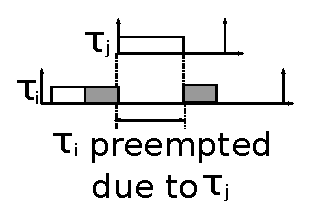
\includegraphics[scale=0.7]{figures/figure8}\caption{\label{fig8}Transactional retry due to release of higher priority
tasks}
\end{figure}
\end{comment}
\end{proof}

\begin{clm}\label{rcm rlease conflict}
Under RCM and G-RMA/LCM, the total retry cost suffered by all transactions in any $\tau_i^x$ during an interval $L\le T_i$ is upper bounded by:
\begin{equation}
RC_{to}(L)=RC(L)+RC_{re}(L)
\label{total rc rcm eq}
\end{equation}
%
where $RC(L)$ and $RC_{re}(L)$ are defined in Claim~\ref{ecm rlease conflict}. $RC(L)$ is calculated by (\ref{eq20}) for RCM, and (\ref{eq60}) for G-RMA/LCM. $RC_{re}(L)$ is calculated by:
\begin{equation}
RC_{re}(L)=\sum_{\forall \tau_j \in \zeta_i^*}\left(\left\lceil\frac{L}{T_j}\right\rceil s_{i_{max}}\right)\label{eq21}
\end{equation}
%
where $\zeta_i^*=\{\tau_j:p_j > p_i \}$.
\end{clm}
\begin{proof}\normalfont
The proof is the same as that for Claim~\ref{ecm rlease conflict}, except that G-RMA uses static priority. Thus, the carried-out jobs will be considered in the  interference with $\tau_i^x$. The carried-in jobs are still not considered because they are released before $r_i^x$. Claim follows.
\end{proof}
\begin{clm}\label{lock free release}
Consider lock-free synchronization. Let $r_{i_{max}}$ be the maximum execution cost of a single iteration of any retry loop of $\tau_i$. $RC_{re}$ under G-EDF  with lock-free synchronization is calculated by~(\ref{eq6}), where $s_{i_{max}}$ is replaced by $r_{i_{max}}$. $RC_{re}$ under G-RMA with lock-free synchronization is calculated by~(\ref{eq21}), where $s_{i_{max}}$ is replaced by $r_{i_{max}}$.
\end{clm}
%
\begin{proof}\normalfont
The interference pattern of higher priority jobs to lower priority jobs is the same in ECM, G-EDF/LCM, and G-EDF with lock-free. The pattern is also the same in RCM, G-RMA/LCM, and G-RMA with lock-free. 
%Claim follows.
\end{proof}


\subsection{PNF versus ECM\label{pnf vs ecm sec}}

\begin{clm}\label{PNF ecf comaprison clm}
In the absence of transitive retry, PNF/G-EDF's schedulability is better or equal to ECM's when conflicting atomic sections have equal lengths.
\end{clm}
\begin{proof}\normalfont
Substitue $RC_{A}(T_{i})$ and $RC_{B}(T_{i})$ in (\ref{utilization comparison})
with (\ref{rc-PNF}) and (\ref{total rc ecm eq}), respectively. Let $\theta_{i}^{ex}=\theta_{i}+\theta_{i}^{*}$, where $\theta_{i}^{*}$
is the set of objects not accessed directly by $\tau_{i}$ but can
cause transactions in $\tau_{i}$ to retry due to transitive retry.
Let $\gamma_{i}^{ex}=\gamma_{i}+\gamma_{i}^{*}$, where $\gamma_{i}^{*}$
is the set of tasks that access objects in $\theta_{i}^{*}$.
Let:
%
\begin{comment}
\begin{eqnarray*}
g(\tau_{i}) & = & \left(\sum_{\forall\tau_{j}\in\gamma_{i}^{*}}\sum_{\theta\in\theta_{i}^{*}}\left(\left\lceil \frac{T_{i}}{T_{j}}\right\rceil \sum_{\forall\bar{s_{j}^{k}(\theta)}}len\left(\bar{s_{j}^{k}(\theta)}\\
& + & s_{max}(\theta)\right)\right)\right) + RC_{re}(T_{i})
\end{eqnarray*}
\begin{eqnarray*}
g(\tau_{i}) & = & \Bigg(\sum_{\forall\tau_{j}\in\gamma_{i}^{*}}\sum_{\theta\in\theta_{i}^{*}}\Bigg(\left\lceil \frac{T_{i}}{T_{j}}\right\rceil \sum_{\forall\bar{s_{j}^{k}(\theta)}}len\Big(\bar{s_{j}^{k}(\theta)}\\
 & + & s_{max}(\theta)\Big)\Bigg)\Bigg)+RC_{re}(T_{i})
\end{eqnarray*}
\end{comment}
\begin{equation*}
g(\tau_{i}) = \left(\sum_{\forall\tau_{j}\in\gamma_{i}^{*}}\sum_{\theta\in\theta_{i}^{*}}\left(\left\lceil \frac{T_{i}}{T_{j}}\right\rceil \sum_{\forall\bar{s_{j}^{k}(\theta)}}len\left(\bar{s_{j}^{k}(\theta)} + s_{max}(\theta)\right)\right)\right)+RC_{re}(T_{i})
\end{equation*}

%
where $RC_{re}$ is given by~(\ref{eq6}). $g(\tau_i)$ includes effect of transitive retry. Let:
%
\begin{equation*}
\eta_{1}(\tau_{i})=\sum_{\forall\tau_{j}\in\gamma_{i}}\sum_{\forall\theta\in\theta_{i}}\left(\sum_{\bar{\forall s_{j}^{k}(\theta)}}len\left(\bar{s_{j}^{k}(\theta)}\right)\right)
\end{equation*}
%
\begin{equation*}
\eta_{2}(\tau_{i})=\sum_{\forall\tau_{j}\in\gamma_{i}}\sum_{\forall\theta\in\theta_{i}}\left(\left\lceil \frac{T_{i}}{T_{j}}\right\rceil \sum_{\forall\bar{s_{j}^{k}(\theta)}}len\left(s_{max}^{j}(\theta)\right)\right)
\end{equation*}
%
%and
%
\begin{equation*}
\eta_{3}(\tau_{i})=\sum_{\forall\tau_{j}\in\gamma_{i}}\sum_{\forall\theta\in\theta_{i}}\left(\left\lceil \frac{T_{i}}{T_{j}}\right\rceil \sum_{\bar{\forall s_{j}^{k}(\theta)}}len\left(\bar{s_{j}^{k}(\theta)}\right)\right)
\end{equation*}
%
By substitution of $g(\tau_{i})$, $\eta_1(\tau_i)$, and $\eta_2(\tau_i)$, and subtraction of $\sum_{\forall \tau_i} \frac{\eta_3(\tau_i)}{T_i}$ from both sides of (\ref{utilization comparison}), we get: 
\begin{equation}
\sum_{\forall \tau_i} \frac{\eta_1(\tau_i)}{T_i} \le \sum_{\forall \tau_i} \frac{\eta_2(\tau_i)+g(\tau_i)}{T_i}
\label{PNF ecm comparison 2}
\end{equation}
Assume that $g(\tau_{i})_{\forall\tau_{i}}\rightarrow0$. From (\ref{PNF ecm comparison 2}), we note that by keeping
every $len(\bar{s_{j}^{k}(\theta)})\le len(s_{max}^{j}(\theta))$
for each $\tau_{i}$, $\tau_{j}\in\gamma_{i}$, and $\theta\in\theta_{i}$,  (\ref{PNF ecm comparison 2}) holds. 
%
Due to G-EDF's dynamic priority, $s_{max}^{j}(\theta)$
can belong to any task other than $\tau_{j}$. By keeping $len(\bar{s_j^k(\theta)})\le len(s_{max}^j(\theta))$, then~\ref{PNF ecm comparison 2} holds. By generalizing this condition to any $s_j^k(\theta)$ and $s_{max}^j(\theta)$, then~\ref{PNF ecm comparison 2} holds if all atomic sections in all tasks have equal lengths. Claim follows.
\end{proof}

\subsection{PNF versus RCM}\label{pnf vs rcm sec}

\begin{clm}\label{clm_pnf_rcm_comp}
In the absence of transitive retry, PNF/G-RMA's schedulability is better or equal to RCM's schedulability when a large number of tasks heavily conflict. PNF's schedulability is improved compared with RCM's, when atomic section length increases as priority increases. 
\end{clm}
\begin{proof}\normalfont
Let $\theta_{i}^{ex}=\theta_{i}+\theta_{i}^{*}$ and $\gamma_{i}^{ex}=\gamma_{i}+\gamma_{i}^{*}$, as defined in the proof of Claim~\ref{PNF ecf comaprison clm}. Substitute $RC_{A}(T_{i})$ and $RC_{B}(T_{i})$ in (\ref{utilization comparison}) with (\ref{rc-PNF}) and (\ref{total rc rcm eq}), respectively. Let: 
%
%\begin{eqnarray*}
%g(\tau_{i}) & =RC_{re}(T_{i})+\Bigg( & \sum_{\forall\tau_{j}\in(\gamma_{i}^{*}\cap\zeta_{i}^{*})}\sum_{\forall\theta\in\theta_{i}^{*}}\left(\left\lceil \frac{T_{i}}{T_{j}}\right\rceil +1\right)\times\\
% &  & \sum_{\forall\bar{s_{j}^{k}(\theta)}}len\left(\bar{s_{j}^{k}(\theta)}+s_{max}^{j}(\theta)\right)\Bigg)
%\end{eqnarray*}
\begin{equation*}
g(\tau_{i}) =RC_{re}(T_{i})+\left(\sum_{\forall\tau_{j}\in(\gamma_{i}^{*}\cap\zeta_{i}^{*})}\sum_{\forall\theta\in\theta_{i}^{*}}\left(\left\lceil \frac{T_{i}}{T_{j}}\right\rceil +1\right)\times \sum_{\forall\bar{s_{j}^{k}(\theta)}}len\left(\bar{s_{j}^{k}(\theta)}+s_{max}^{j}(\theta)\right)\right)
\end{equation*}
%
where $RC_{re}$ and $\zeta_i^*$ are defined by~(\ref{eq21}). $g(\tau_i)$ includes effect of transitive retry. 
Let $\gamma_{i}=\zeta_{i}^{*}\cup\bar{\zeta_{i}}$, where $\bar{\zeta_{i}}=\left\{ \tau_{j}:\left(\tau_{j}\ne\tau_{i}\right)\wedge\left(p_{j}<p_{i}\right)\right\} $,
thus $\zeta_{i}^{*}\cap\bar{\zeta_{i}}=\phi$.

Let:
%
\begin{equation*}
\eta_{1}(\tau_{i})=\sum_{\forall\tau_{j}\in(\gamma_{i}\cap\zeta_{i}^{*})}\sum_{\forall\theta\in\theta_{i}}\left(\left(\left\lceil \frac{T_{i}}{T_{j}}\right\rceil +1\right)\sum_{\bar{\forall s_{j}^{k}(\theta)}}len\left(\bar{s_{j}^{k}(\theta)}\right)\right)
\end{equation*}
%
\begin{equation*}
\eta_{2}(\tau_{i})=\sum_{\forall\tau_{j}\in(\gamma_{i}\cap\bar{\zeta_{i}})}\sum_{\forall\theta\in\theta_{i}}\left(\left(\left\lceil \frac{T_{i}}{T_{j}}\right\rceil +1\right)\sum_{\bar{\forall s_{j}^{k}(\theta)}}len\left(\bar{s_{j}^{k}(\theta)}\right)\right)
\end{equation*}
%
%and
%
%\begin{eqnarray*}
%\eta_{3}(\tau_{i}) & = & \sum_{\forall\tau_{j}\in(\gamma_{i}\cap\zeta_{i}^{*})}\sum_{\forall\theta\in\theta_{i}}\Bigg(\left(\left\lceil \frac{T_{i}}{T_{j}}\right\rceil +1\right)\times\\
% &  & \sum_{\forall\bar{s_{j}^{k}(\theta)}}len\left(\bar{s_{j}^{k}(\theta)}+s_{max}^{j}(\theta)\right)\Bigg)
%\end{eqnarray*}
\begin{equation*}
\eta_{3}(\tau_{i}) = \sum_{\forall\tau_{j}\in(\gamma_{i}\cap\zeta_{i}^{*})}\sum_{\forall\theta\in\theta_{i}}\left(\left(\left\lceil \frac{T_{i}}{T_{j}}\right\rceil +1\right)\times \sum_{\forall\bar{s_{j}^{k}(\theta)}}len\left(\bar{s_{j}^{k}(\theta)}+s_{max}^{j}(\theta)\right)\right)
\end{equation*}
%
By substitution of $g(\tau_i)$, $\eta_1(\tau_i)$, $\eta_2(\tau_i)$, and $\eta_3(\tau_i)$ in (\ref{utilization comparison}):
%
\begin{equation}
\sum_{\forall\tau_{i}}\frac{\eta_{1}(\tau_{i})+\eta_{2}(\tau_{i})}{T_{i}}\le\sum_{\forall\tau_{i}}\frac{\eta_{3}(\tau_{i})+g(\tau_{i})}{T_{i}}
\label{PNF rcm comparison 3}
\end{equation}
%
When tasks with deadlines equal to periods are scheduled with G-RMA, $T_{j}>T_{i}$ if $p_{j}<p_{i}$. So, for each $\tau_{j}\in\bar{\zeta_{i}}$, $\left\lceil \frac{T_{i}}{T_{j}}\right\rceil =1$. Then:
%
\begin{equation}
\eta_{2}(\tau_{i})=2\sum_{\forall\tau_{j}\in(\gamma_{i}\cap\bar{\zeta_{i}})}\sum_{\forall\theta\in\theta_{i}}\sum_{\bar{\forall s_{j}^{k}(\theta)}}len\left(\bar{s_{j}^{k}(\theta)}\right)
\label{PNF rcm comparison 5}
\end{equation}
%
Let:
%
\begin{equation*}
\eta_{4}(\tau_{i})=\sum_{\forall\tau_{j}\in(\gamma_{i}\cap\zeta_{i}^{*})}\sum_{\forall\theta\in\theta_{i}}\left(\left\lceil \frac{T_{i}}{T_{j}}\right\rceil +1\right)\sum_{\forall\bar{s_{j}^{k}(\theta)}}len\left(s_{max}^{j}(\theta)\right)
\end{equation*}
%
By substitution of~(\ref{PNF rcm comparison 5}) and subtraction of $\sum_{\forall \tau_i} \frac{\eta_1 (\tau_i)}{T_i}$ from both sides of~(\ref{PNF rcm comparison 3}), we get:
%
\begin{equation}
2\sum_{\forall\tau_{i}}\frac{\eta_{2}(\tau_{i})}{T_{i}}\le\sum_{\forall\tau_{i}}\frac{\eta_{4}(\tau_{i})+g(\tau_{i})}{T_{i}}
\label{PNF rcm comparison 4}
\end{equation}
%
Assume that $g(\tau_{i})_{\forall\tau_{i}}\rightarrow0$. From (\ref{PNF rcm comparison 4}), we note that when higher priority jobs increasingly conflict with lower priority jobs, (\ref{PNF rcm comparison 4}) tends to hold. (\ref{PNF rcm comparison 4}) also tends to hold if $len(\bar{s_{max}^j(\theta)})$ in the right hand side of (\ref{PNF rcm comparison 4}) is larger than $len(\bar{s_j^k(\theta)})$ in the left hand side of (\ref{PNF rcm comparison 4}), which means atomic section length increases as priority increases. Claim follows.
\end{proof}

\subsection{PNF versus G-EDF/LCM}

\begin{clm}\label{sub:pnf_lcm_edf_comp}
In the absence of transitive retry, PNF/EDF's schedulability is equal or better than G-EDF/LCM's if the conflicting atomic section lengths are approximately equal and all $\alpha$ terms approach 1.

\end{clm}
\begin{proof}\normalfont
Assume that $\eta_{1}(\tau_i)$ and $\eta_{3}(\tau_i)$ are the same as that defined in the proof
of Claim~\ref{PNF ecf comaprison clm}. Let:
%\begin{eqnarray*}
%g(\tau_{i}) & = & \Bigg(\sum_{\forall\tau_{j}\in\gamma_{i}^{*}}\sum_{\theta\in\theta_{i}^{*}}\Bigg(\left\lceil \frac{T_{i}}{T_{j}}\right\rceil \sum_{\forall\bar{s_{j}^{k}(\theta)}}len\Big(\bar{s_{j}^{k}(\theta)}\\
% & + & \alpha_{max}^{ji}s_{max}(\theta)\Big)\Bigg)\Bigg)+RC_{re}(T_{i})
%\end{eqnarray*}
\begin{equation*}
g(\tau_{i}) = \left(\sum_{\forall\tau_{j}\in\gamma_{i}^{*}}\sum_{\theta\in\theta_{i}^{*}}\left(\left\lceil \frac{T_{i}}{T_{j}}\right\rceil \sum_{\forall\bar{s_{j}^{k}(\theta)}}len\left(\bar{s_{j}^{k}(\theta)} + \alpha_{max}^{ji}s_{max}(\theta)\right)\right)\right)+RC_{re}(T_{i})
\end{equation*}

\[
\eta_{2}(\tau_{i})=\sum_{\forall\tau_{j}\in\gamma_{i}}\sum_{\forall\theta\in\theta_{i}}\left(\left\lceil \frac{T_{i}}{T_{j}}\right\rceil \sum_{\forall\bar{s_{j}^{k}(\theta)}}len\left(\alpha_{max}^{jl}s_{max}^{j}(\theta)\right)\right)
\]
where $\alpha_{max}^{jl}$ is defined in~(\ref{eq78}). Following the same steps in the proof of Claim~\ref{PNF ecf comaprison clm}, we get:
\begin{equation}
\sum_{\forall\tau_{i}}\frac{\eta_{1}(\tau_{i})}{T_{i}}\le\sum_{\forall\tau_{i}}\frac{\eta_{2}(\tau_{i})+g(\tau_{i})}{T_{i}}\label{eq:pnf_lcm_edf_comp}
\end{equation}
Assume that $g(\tau_{i})_{\forall\tau_{i}}\rightarrow0$. Thus, we ignore the effect of transitive retry and retry cost due to the release of higher priority jobs. Let $len(\bar{s_{j}^{k}(\theta)})=s_{max}^{j}(\theta)=s$,
and $\alpha_{max}^{jl}=\alpha_{max}^{iy}=1$ in (\ref{eq:pnf_lcm_edf_comp}). Then, PNF/EDF's schedulability equals LCM/EDF's schedulability if
$\left\lceil \frac{T_{i}}{T_{j}}\right\rceil =1,\,\forall\tau_{i},\tau_{j}$
(which means equal periods for all tasks). If $\left\lceil \frac{T_{i}}{T_{j}}\right\rceil >1,\,\forall\tau_{i},\tau_{j}$,
PNF/EDF's schedulability is better than LCM/EDF's. PNF/EDF's schedulability  becomes more better than LCM/EDF's schedulability if $g(\tau_{i})$
is not zero. Claim follows.
\end{proof}

%\begin{comment}
\subsection{PNF versus G-RMA/LCM}

\begin{clm}\label{sub:pnf_lcm_rma_comp}
%
In the absence of transitive retry, PNF's schedulability is equal or better than G-RMA/LCM's if: 1) lower priority tasks suffer increasing number of conflicts from higher priority tasks, 2) the lengths of the atomic sections increase as task priorities increase, and 3) $\alpha$ terms increase.
%
\end{clm}
\begin{proof}\normalfont
Assume that $g(\tau_{i})$, $\eta_{1}(\tau_{i})$, and $\eta_{2}(\tau_{i})$ are the same as in the proof of Claim~\ref{clm_pnf_rcm_comp}. Let:
%\begin{eqnarray*}
%\eta_{3}(\tau_{i}) & = & \sum_{\forall\tau_{j}\in(\gamma_{i}\cap\zeta_{i}^{*})}\sum_{\forall\theta\in\theta_{i}}\Bigg(\left(\left\lceil \frac{T_{i}}{T_{j}}\right\rceil +1\right)\times\\
% &  & \sum_{\forall\bar{s_{j}^{k}(\theta)}}len\left(\bar{s_{j}^{k}(\theta)}+\alpha_{max}^{jl}s_{max}^{j}(\theta)\right)\Bigg)
%\end{eqnarray*}
\begin{equation*}
\eta_{3}(\tau_{i}) = \sum_{\forall\tau_{j}\in(\gamma_{i}\cap\zeta_{i}^{*})}\sum_{\forall\theta\in\theta_{i}}\left(\left(\left\lceil \frac{T_{i}}{T_{j}}\right\rceil +1\right)\times \sum_{\forall\bar{s_{j}^{k}(\theta)}}len\left(\bar{s_{j}^{k}(\theta)}+\alpha_{max}^{jl}s_{max}^{j}(\theta)\right)\right)
\end{equation*}
%and
%\begin{eqnarray*}
%\eta_{4}(\tau_{i}) & = & \sum_{\forall\tau_{j}\in(\gamma_{i}\cap\zeta_{i}^{*})}\sum_{\forall\theta\in\theta_{i}}\Bigg(\left(\left\lceil \frac{T_{i}}{T_{j}}\right\rceil +1\right)\\
% & \times & \sum_{\forall\bar{s_{j}^{k}(\theta)}}len\left(\alpha_{max}^{jl}s_{max}^{j}(\theta)\right)\Bigg)
%\end{eqnarray*}
\begin{equation*}
\eta_{4}(\tau_{i}) = \sum_{\forall\tau_{j}\in(\gamma_{i}\cap\zeta_{i}^{*})}\sum_{\forall\theta\in\theta_{i}}\left(\left(\left\lceil \frac{T_{i}}{T_{j}}\right\rceil +1\right) \times \sum_{\forall\bar{s_{j}^{k}(\theta)}}len\left(\alpha_{max}^{jl}s_{max}^{j}(\theta)\right)\right)
\end{equation*}

Following the steps of Claim~\ref{clm_pnf_rcm_comp}'s proof, 
$\therefore$(\ref{utilization comparison}) becomes:
\begin{equation}
2\sum_{\forall\tau_{i}}\frac{\eta_{2}(\tau_{i})}{T_{i}}\le\sum_{\forall\tau_{i}}\frac{\eta_{4}(\tau_{i})+g(\tau_{i})}{T_{i}}\label{pnf-lcm-rma-comp-2}
\end{equation}
Assume that the effect of transitive retry and retry cost due
to the release of higher priority jobs is negligible ($g(\tau_{i})\rightarrow0$). (\ref{pnf-lcm-rma-comp-2})
holds if: 1) the contention from higher priority jobs to lower priority
jobs increases because of the $\left\lceil \frac{T_{i}}{T_{j}}\right\rceil +1$
term in the right hand side of (\ref{pnf-lcm-rma-comp-2}); 2) $\alpha$ terms
approach 1; and 3) the lengths of the atomic sections increase as priority
increases. 
%
This makes $len(s_{max}^{j}(\theta))$ in (\ref{pnf-lcm-rma-comp-2})'s right 
side to be greater than $len(\bar{s_{j}^{k}(\theta)})$ in (\ref{pnf-lcm-rma-comp-2})'s left  side.
Claim follows.
\end{proof}
%\end{comment}

\subsection{PNF versus Lock-free Synchronization\label{pnf vs lock free sec}}

Lock-free synchronization~\cite{key-5,stmconcurrencycontrol:emsoft11} accesses only one object. Thus, the number of accessed objects per transaction in PNF is limited to one. This allows us to compare the schedulability of PNF with the lock-free algorithm. 

$RC_{B}(T_{i})$ in (\ref{utilization comparison}) is replaced with:
%
\begin{equation}
\sum_{\forall\tau_{j}\in\gamma_{i}}\Bigg(\left(\left\lceil \frac{T_{i}}{T_{j}}\right\rceil +1\right)\beta_{i,j}r_{max}\Bigg)+RC_{re}(T_{i})
\label{lock-free rc}
\end{equation}
%
where $\beta_{i,j}$ is the number of retry loops of $\tau_{j}$ that access the same object as accessed by some retry loop of $\tau_{i}$~\cite{key-5}. $r_{max}$ is the maximum execution cost of a single iteration of any retry loop of any task~\cite{key-5}. $RC_{re}(T_i)$ is defined in Claim~\ref{lock free release}. Lock-free synchronization does not depend on priorities  of tasks. Thus,~(\ref{lock-free rc}) applies for both G-EDF and G-RMA systems.


%%
\begin{clm}\label{PNF lock-free comparison}
Let $r_{max}$ be the maximum execution cost of a single iteration of any retry loop of any task~\cite{key-5}. Let $s_{max}$ be the maximum transaction length in all tasks. Assume that each transaction under PNF accesses only one object for once. The schedulability of PNF with either G-EDF or G-RMA scheduler is better or equal to the schedulability of lock-free
synchronization if $s_{max}/r_{max}\le 1$.
\end{clm}
\begin{proof}\normalfont
The assumption in Claim~\ref{PNF lock-free comparison} is made to enable a comparison between PNF and lock-free. Let $RC_{A}(T_{i})$ in (\ref{utilization comparison}) be replaced
with (\ref{rc-PNF}) and $RC_{B}(T_{i})$ be replaced with (\ref{lock-free rc}).
To simplify comparison, (\ref{rc-PNF}) is upper bounded by:
%
\begin{equation*}
RC(T_{i})=\sum_{\tau_{j}\in\gamma_{i}}\left(\left(\left\lceil \frac{T_{i}}{T_{j}}\right\rceil +1\right)\beta_{i,j}^* s_{max}\right)
\end{equation*}
%
where $\beta_{i,j}^*$ is the number of times transactions in $\tau_j$ accesses shared objects with $
\tau_i$. Thus, $\beta_{i,j}^* = \beta_{i,j}$, and (\ref{utilization comparison}) will be:
%\begin{eqnarray}
%\sum_{\forall\tau_{i}}\frac{\sum_{\tau_{j}\in\gamma_{i}}\left(\left(\left\lceil \frac{T_{i}}{T_{j}}\right\rceil +1\right)\beta_{i,j}s_{max}\right)}{T_{i}} & \le\nonumber \\
%\sum_{\forall\tau_{i}}\frac{\sum_{\forall\tau_{j}\in\gamma_{i}}\left(\left\lceil \frac{T_{i}}{T_{j}}\right\rceil +1\right)\beta_{i,j}r_{max}+RC_{re}(\tau_i)}{T_{i}}\label{eq:PNF lock-free comparison}
%\end{eqnarray}
\begin{equation}
\sum_{\forall\tau_{i}}\frac{\sum_{\tau_{j}\in\gamma_{i}}\left(\left(\left\lceil \frac{T_{i}}{T_{j}}\right\rceil +1\right)\beta_{i,j}s_{max}\right)}{T_{i}}\le \sum_{\forall\tau_{i}}\frac{\sum_{\forall\tau_{j}\in\gamma_{i}}\left(\left\lceil \frac{T_{i}}{T_{j}}\right\rceil +1\right)\beta_{i,j}r_{max}+RC_{re}(\tau_i)}{T_{i}}\label{eq:PNF lock-free comparison}
\end{equation}

From (\ref{eq:PNF lock-free comparison}), we note that if $s_{max}\le r_{max}$,
then (\ref{eq:PNF lock-free comparison}) holds. 
%Claim follows.
\end{proof}


\section{Conclusion}\label{pnf_conclusion}

Transitive retry increases transactional retry cost under ECM, RCM, and LCM. PNF avoids transitive retry by avoiding   transactional preemptions. PNF reduces the priority of aborted transactions to enable other tasks to execute, increasing processor usage. Executing transactions are not preempted due to the release of higher priority jobs. On the negative side of PNF, higher priority jobs can be blocked by executing transactions of lower priority jobs. 

EDF/PNF's schedulability is equal or better than ECM's when atomic section lengths are almost equal. RMA/PNF's schedulability is equal or better than RCM's when lower priority jobs suffer greater conflicts from higher priority ones. Similar conditions hold for the schedulability comparison between PNF and LCM, in addition to the increase of $\alpha$ terms to 1. This is logical as LCM with G-EDF (G-RMA) defaults to ECM (RCM) with $\alpha\rightarrow 1$. For PNF's schedulability to be equal or better than lock-free, the upper bound on $s_{max}/r_{max}$ must be 1, instead of 0.5 under ECM and RCM. 


%%%%%%%%%%%%%%%%%%%%%%%%%%%%%%%%

\chapter{\label{ch_exp}Implementation and Experimental Evaluations}
\markright{Mohammed El-Shambakey \hfill Chapter~\ref{ch_exp}. Experiments \hfill}

Having established upper bounds for retry cost of different contention managers, and the conditions under which each one is prefered. We now would like to understand how each CM retries in practice (i.e., on average) compared with that of competitor methods. Since this can only be understood experimentally, we implement ECM, RCM, LCM, PNF and lock-free and conduct experimental studies.

The rest of this Chapter is organized as follow: Section~\ref{sec:experimental_setup} outlines the experimental settings and used task sets for comparing different contention managers and lock-free. Section~\ref{sec:final_results} discusses experimental results.

\section{Experimental Setup}\label{sec:experimental_setup}
We used the ChronOS real-time Linux kernel~\cite{dellinger2011chronos}
and the RSTM library~\cite{marathe2006lowering}. We modified RSTM to include implementations of ECM, RCM, LCM, and PNF contention managers, and modified ChronOS to include implementations of G-EDF and G-RMA schedulers. 

For the retry-loop lock-free implementation,
we used a loop that reads an object and attempts to write to the object using a compare-and-swap (CAS) instruction. The task retries until the CAS succeeds. 
%We call this lock-free operation, CAS-loop operation.

We use an 8 core, 2GHz AMD Opteron platform. The average time
taken for one write operation by RSTM on any
core is 0.0129653375$\mu s$, and the average time taken
by one CAS-loop operation on any core is 0.0292546250 $\mu s$.

We used 3 sets of 4, 8 and 20 tasks. The structure of these tasks are shown in Table~\ref{pnf_task_sets_table}. Each task runs in its own thread and has a set of atomic sections. Atomic section properties are probabilistically controlled (for experimental evaluation) using three parameters: the maximum and minimum lengths of any atomic section within the task, and the total length of atomic sections within any task. As lock-free cannot access more than one object in one atomic operation, tasks share one object per transaction when lock-free is included in comparison. Then, CMs are compared against each other discarding lock-free.

\begin{flushleft}
\begin{table}[htbp]
\begin{centering}
\caption{\label{pnf_task_sets_table}Task sets \label{tab:Task-sets-a)pnf4}a) 4 tasks. \label{tab:Task-sets-a)pnf8}b)
8 tasks. \label{tab:Task-sets-a)pnf20}c) 20 tasks.}

\begin{tabular}{|c|c|}
\multicolumn{2}{c}{(a)}\tabularnewline
\hline 
$P_{i}(\mu s)$ & $c_{i}(\mu s)$\tabularnewline
\hline 
1000000 & 227000\tabularnewline
\hline 
1500000 & 410000\tabularnewline
\hline 
3000000 & 299000\tabularnewline
\hline 
5000000 & 500000\tabularnewline
\hline 
\end{tabular}~% 
\begin{tabular}{|c|c|}
\multicolumn{2}{c}{(b)}\tabularnewline
\hline 
$P_{i}(\mu s)$ & $c_{i}(\mu s)$\tabularnewline
\hline 
1500000 & 961000\tabularnewline
\hline 
1875000 & 175000\tabularnewline
\hline 
2500000 & 205000\tabularnewline
\hline 
3000000 & 129000\tabularnewline
\hline 
3750000 & 117000\tabularnewline
\hline 
5000000 & 269000\tabularnewline
\hline 
7500000 & 118000\tabularnewline
\hline 
15000000 & 609000\tabularnewline
\hline 
\end{tabular}~% 
\begin{tabular}{|c|c|}
\multicolumn{2}{c}{(c)}\tabularnewline
\hline 
$P_{i}(\mu s)$ & $c_{i}(\mu s)$\tabularnewline
\hline 
375000 & 9000\tabularnewline
\hline 
400000 & 8000\tabularnewline
\hline 
500000 & 8000\tabularnewline
\hline 
600000 & 14000\tabularnewline
\hline 
625000 & 375000\tabularnewline
\hline 
750000 & 19000\tabularnewline
\hline 
1000000 & 26000\tabularnewline
\hline 
1200000 & 17000\tabularnewline
\hline 
1250000 & 21000\tabularnewline
\hline 
1500000 & 33000\tabularnewline
\hline 
1875000 & 39000\tabularnewline
\hline 
2000000 & 43000\tabularnewline
\hline 
2500000 & 18000\tabularnewline
\hline 
3000000 & 90000\tabularnewline
\hline 
3750000 & 28000\tabularnewline
\hline 
5000000 & 126000\tabularnewline
\hline 
7500000 & 231000\tabularnewline
\hline 
10000000 & 407000\tabularnewline
\hline 
15000000 & 261000\tabularnewline
\hline 
30000000 & 369000\tabularnewline
\hline 
375000 & 8000\tabularnewline
\hline 
30000000 & 407000\tabularnewline
\hline 
\end{tabular}
\par\end{centering}

\end{table}

\par\end{flushleft}
 
The difficulty in testing with PNF is to incur transitive retry cases. Tasks are arranged in non-decreasing order of periods, and each task shares objects only with the previous and next tasks. Each task begins with an atomic section. Thus, increasing the opportunity of transitive retry.



\section{Results}\label{sec:final_results}

Figure~\ref{fig:pnf_results_1_obj_all} shows average retry cost under ECM, RCM, LCM, PNF and lock-free for each task set. Figure~\ref{fig:pnf_results_1_obj_without_lock_free} shows average retry cost for only contention managers for each task set. The $x$-axis has three parameters $a,b,c$. $a$ specifies the relative total length of all atomic sections to the length of the task. $b$ specifies the maximum relative length of any atomic section to the length of the task. $c$ specifies the minimum relative length of any atomic section to the length of the task. Each data point in the figure has a confidence level of 0.95.
Only one object per transaction is shared in Figures~\ref{fig:pnf_results_1_obj_all} and~\ref{fig:pnf_results_1_obj_without_lock_free}.

Lock-free is the longest technique as it provides no conflict resolution. PNF better or comparable retry cost than ECM, RCM and LCM. As we move from 4 to 8 to 20 task set, retry costs of different contention managers get closer to each other. This is explained by noting that each task set in Table~\ref{pnf_task_sets_table} is organized in non-decreasing order of periods, and $c_i/T_i$ for almost each $\tau_i$ is low. Besides, each task shares objects only with the previous and next tasks, and tasks are released at the same time to enforce transitive retry. While the first instances of all tasks have a high potential of conflict, the contention level decreases with time for higher number of tasks. Thus, for the 20 task set, contention level is the lowest. Hence, retry costs of all contention managers get closer as number of tasks increases.

We compared retry cost for different contention managers with multiple objects per transaction and different levels of read/writer operations. Figure~\ref{fig:cm_20obj_per_tx_40wr} shows retry cost of the three task sets sharing 20 objects per transaction, with 40\% write operations and 60\% read operations. The same experiment is repeated in Figure~\ref{fig:cm_20obj_per_tx_80wr} with 80\% write operations, and 20\% read operations. Figure~\ref{fig:cm_20obj_per_tx_100wr} repeats the same experiment with 100\% write operations. The same previous three experiments were repeated in Figures~\ref{fig:cm_40obj_per_tx_40wr},~\ref{fig:cm_40obj_per_tx_80wr} and~\ref{fig:cm_40obj_per_tx_100wr} with 40 objects per transaction. Figures~\ref{fig:cm_20obj_per_tx_40wr} to~\ref{fig:cm_40obj_per_tx_100wr} show consistent trends with Figure~\ref{fig:pnf_results_1_obj_without_lock_free} except that retry cost of PNF is shorter than the others even with increasing number of tasks. For the 20 task set, PNF retry cost is a little shorter than LCM, but much better than ECM and RCM. This happens because of sharing multiple objects per transaction. Thus, contention level is increased than in sharing 1 object per transaction. Besides, transitive retry exists which makes PNF better than the others.
%%%%%%%%%%%%%%%%%%%%%%%%%%%%%%%%%%%%%%%%%%%%%%%%%%%%%%%

\begin{figure}
\centering

\subfigure[4 tasks]{
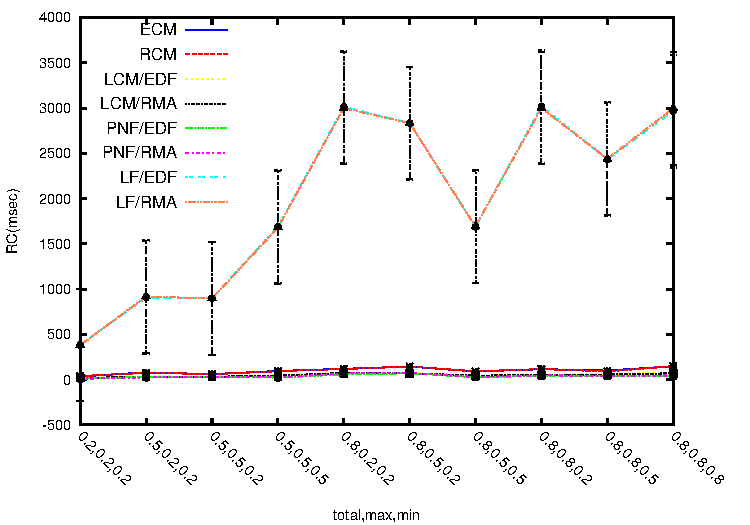
\includegraphics[scale=0.7]
{figures/Abr_dur_4t_5obj_all_100wr}
\label{fig:results_1_obj_all_4_tasks}
}
~
\subfigure[8 tasks]{
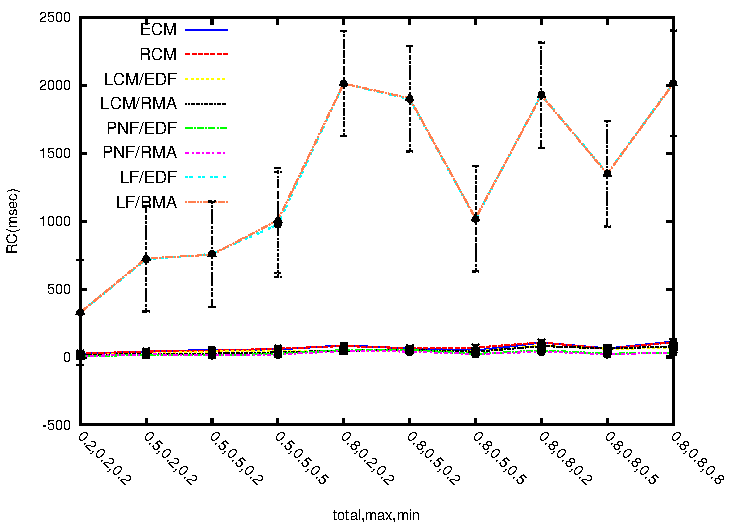
\includegraphics[scale=0.7]
{figures/Abr_dur_8t_9obj_all_100wr}
\label{fig:results_1_obj_all_8_tasks}
}
~
\subfigure[20 tasks]{
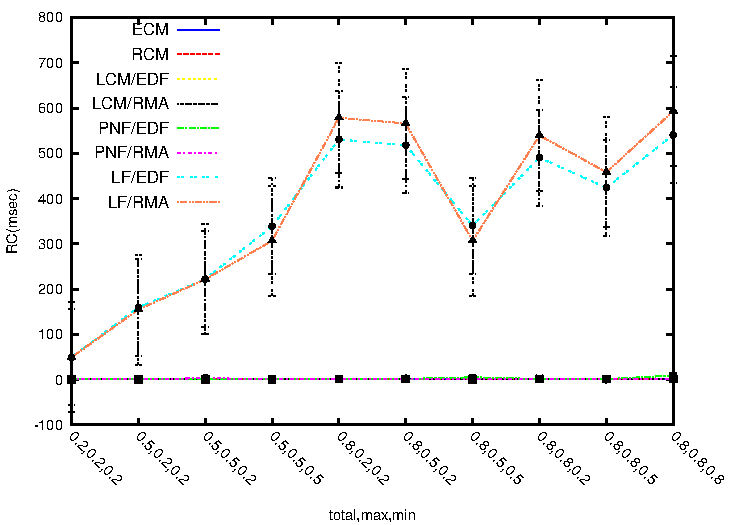
\includegraphics[scale=0.7]
{figures/Abr_dur_20t_21obj_all_100wr}
\label{fig:results_1_obj_all_20_tasks}
}
\caption{Average retry cost for 1 object per transaction for different values of total, maximum and minimum atomic section length under all synchronization techniques}
\label{fig:pnf_results_1_obj_all}
\end{figure}

\begin{figure}
\centering

\subfigure[4 tasks]{
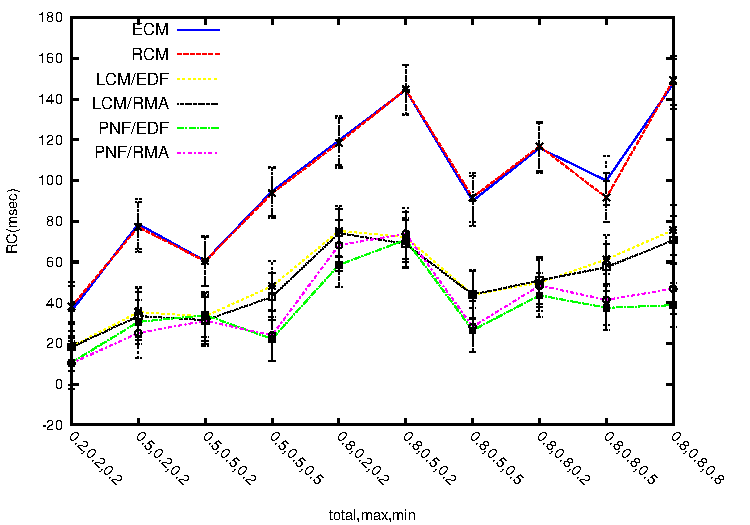
\includegraphics[scale=0.7]
{figures/Abr_dur_4t_5obj_100wr}
\label{fig:pnf_results_1_obj_cm_4t}
}
~
\subfigure[8 tasks]{
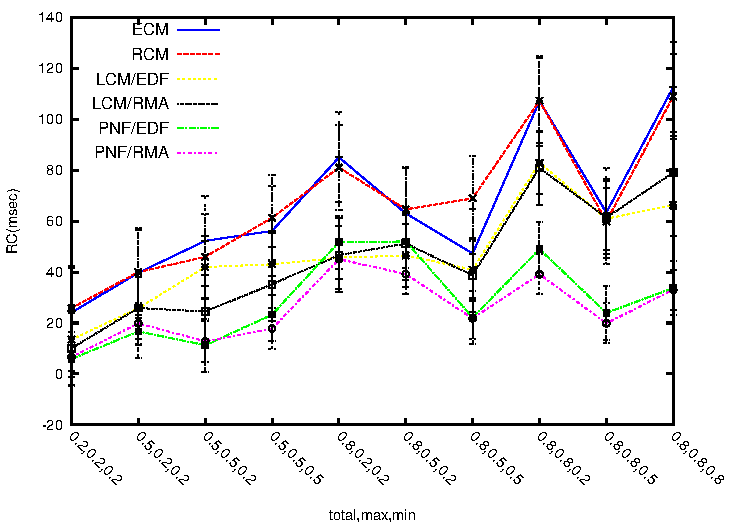
\includegraphics[scale=0.7]
{figures/Abr_dur_8t_9obj_100wr}
\label{fig:pnf_results_1_obj_cm_8t}
}
~
\subfigure[20 tasks]{
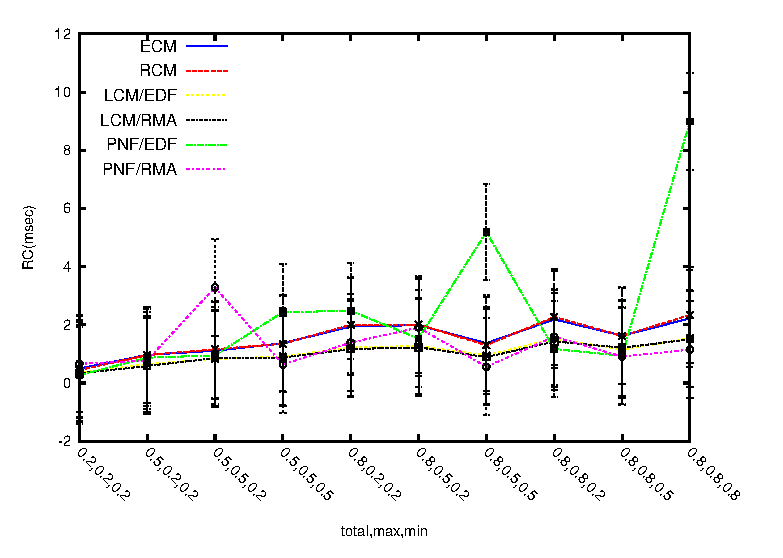
\includegraphics[scale=0.7]
{figures/Abr_dur_20t_21obj_100wr}
\label{fig:pnf_results_1_obj_cm_20t}
}
\caption{Average retry cost for 1 object per transaction for different values of total, maximum and minimum atomic section length under contention managers only}
\label{fig:pnf_results_1_obj_without_lock_free}
\end{figure}
%%%%%%%%%%%%%%%%%%%%%%%%%%%%%%%%
\begin{figure}
\centering

\subfigure[4 tasks]{
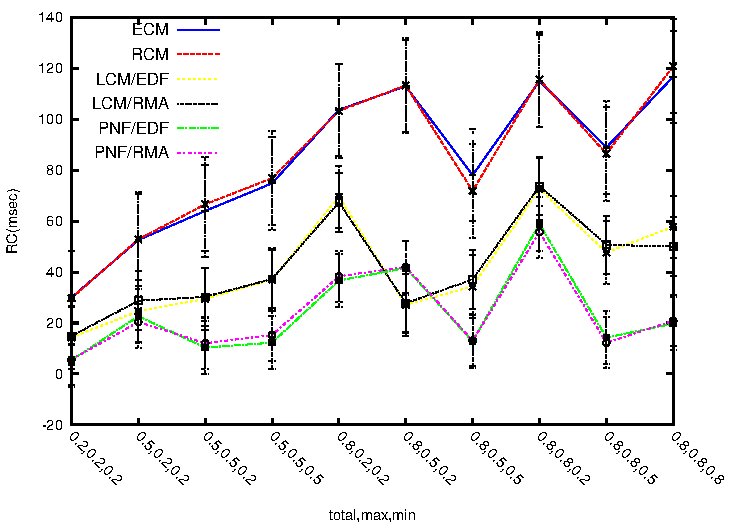
\includegraphics[scale=0.7]
{figures/Abr_dur_4t_50obj_40wr}
\label{fig:4t_ecm_rcm_lcm_pnf_50obj_40wr}
}
~
\subfigure[8 tasks]{
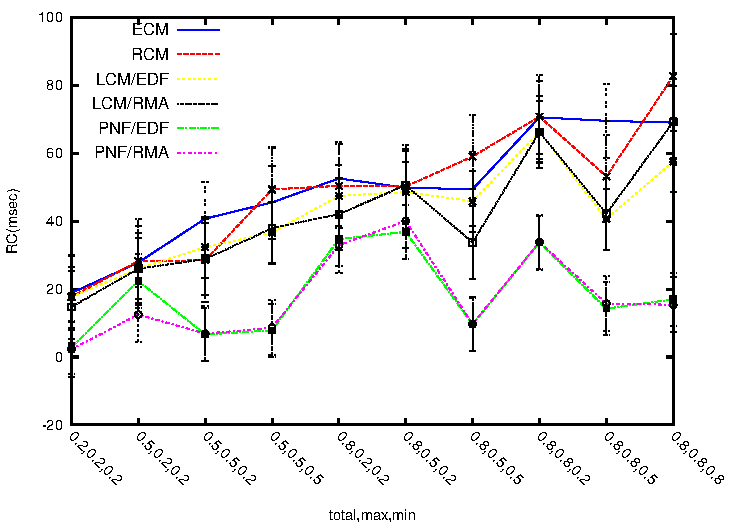
\includegraphics[scale=0.7]
{figures/Abr_dur_8t_90obj_40wr}
\label{fig:8t_ecm_rcm_lcm_pnf_90obj_40wr}
}
~
\subfigure[20 tasks]{
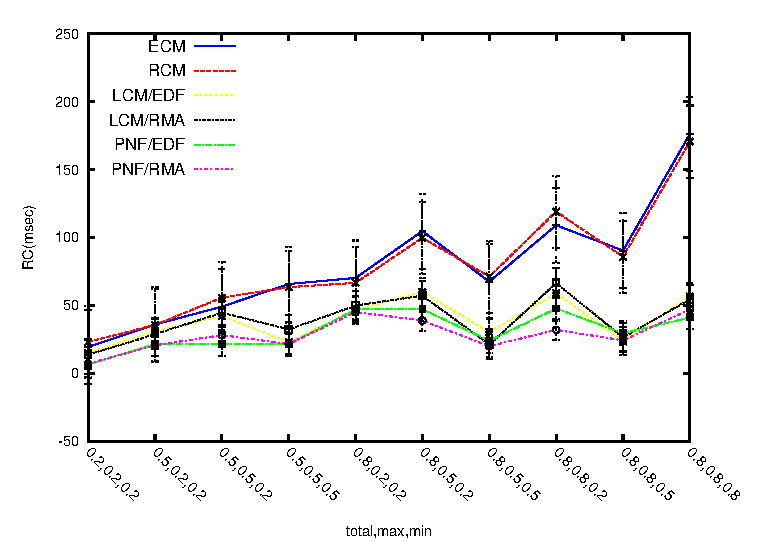
\includegraphics[scale=0.7]
{figures/Abr_dur_20t_210obj_40wr}
\label{fig:20t_ecm_rcm_lcm_pnf_210obj_40wr}
}
\caption{Average retry cost for 20 objects per transaction, 40\% write operations for different values of total, maximum and minimum atomic section length under different CMs}
\label{fig:cm_20obj_per_tx_40wr}
\end{figure}
%%%%%%%%%%%%%%%%%%%%%%%%%%%%%%%%%%%%%%%%%%%%%%%%%%%%%%
%%%%%%%%%%%%%%%%%%%%%%%%%%%%%%%%
\begin{figure}
\centering

\subfigure[4 tasks]{
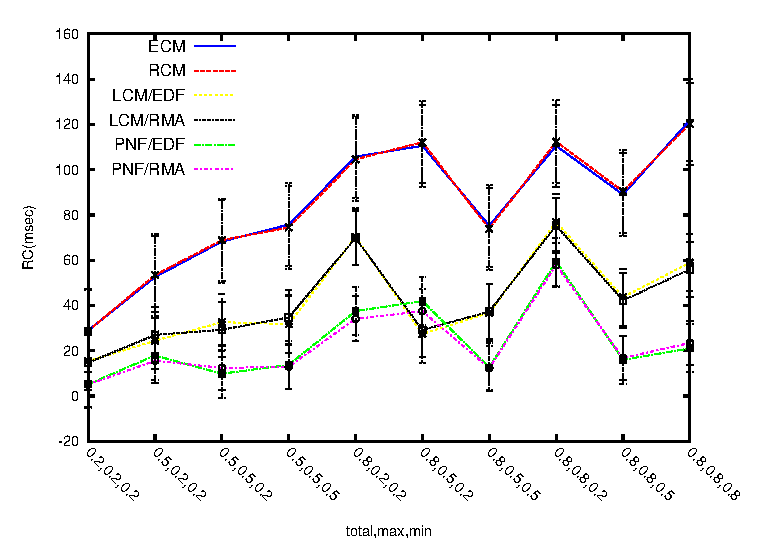
\includegraphics[scale=0.7]
{figures/Abr_dur_4t_50obj_80wr}
\label{fig:4t_ecm_rcm_lcm_pnf_50obj_80wr}
}
~
\subfigure[8 tasks]{
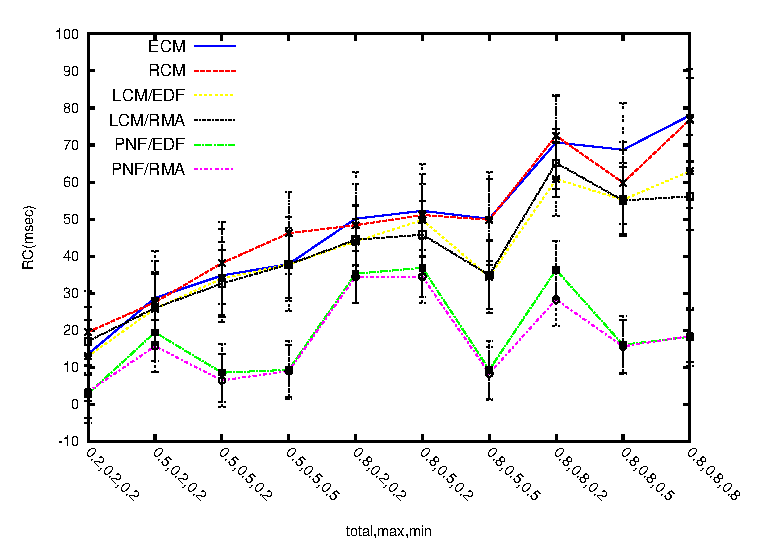
\includegraphics[scale=0.7]
{figures/Abr_dur_8t_90obj_80wr}
\label{fig:8t_ecm_rcm_lcm_pnf_90obj_80wr}
}
~
\subfigure[20 tasks]{
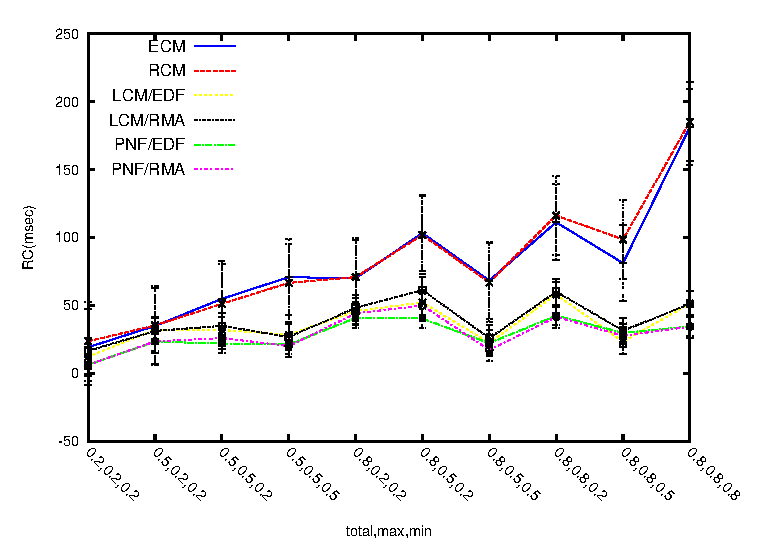
\includegraphics[scale=0.7]
{figures/Abr_dur_20t_210obj_80wr}
\label{fig:20t_ecm_rcm_lcm_pnf_210obj_80wr}
}
\caption{Average retry cost for 20 objects per transaction, 80\% write operations for different values of total, maximum and minimum atomic section length under different CMs}
\label{fig:cm_20obj_per_tx_80wr}
\end{figure}
%%%%%%%%%%%%%%%%%%%%%%%%%%%%%%%%%%%%%%%%%%%%%%%%%%%%%%
\begin{figure}
\centering

\subfigure[4 tasks]{
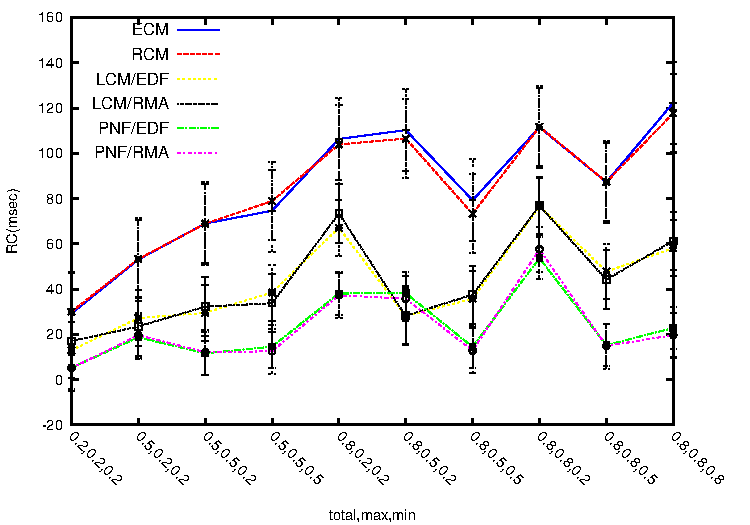
\includegraphics[scale=0.7]
{figures/Abr_dur_4t_50obj_100wr}
\label{fig:4t_ecm_rcm_lcm_pnf_50obj_100wr}
}
~
\subfigure[8 tasks]{
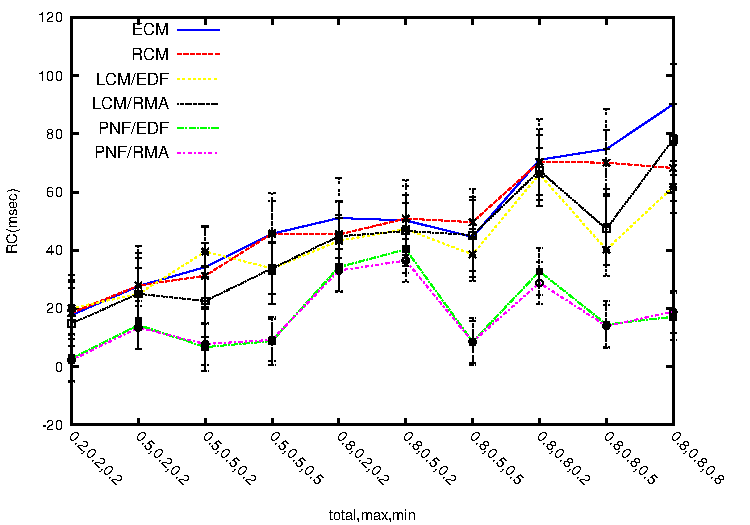
\includegraphics[scale=0.7]
{figures/Abr_dur_8t_90obj_100wr}
\label{fig:8t_ecm_rcm_lcm_pnf_90obj_100wr}
}
~
\subfigure[20 tasks]{
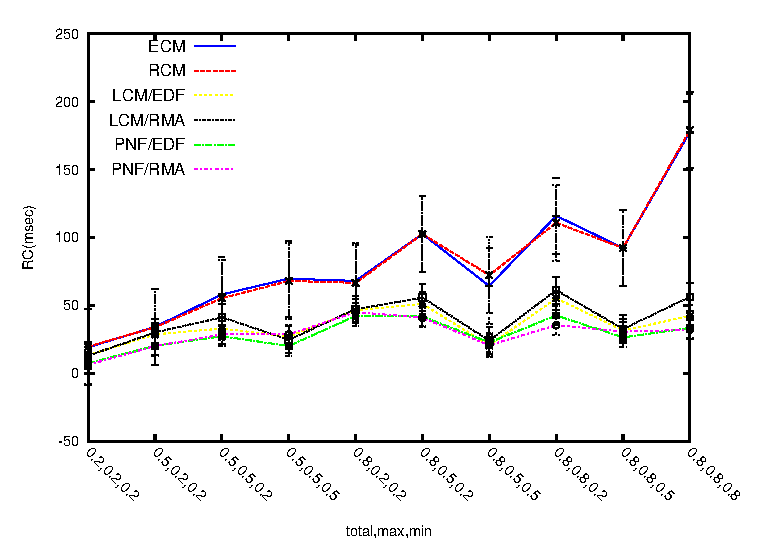
\includegraphics[scale=0.7]
{figures/Abr_dur_20t_210obj_100wr}
\label{fig:20t_ecm_rcm_lcm_pnf_210obj_100wr}
}
\caption{Average retry cost for 20 objects per transaction, 100\% write operations for different values of total, maximum and minimum atomic section length under different CMs}
\label{fig:cm_20obj_per_tx_100wr}
\end{figure}
%%%%%%%%%%%%%%%%%%%%%%%%%%%%%%%%%%%%%%%%%%%%%%%%%%%%%%
\begin{figure}
\centering

\subfigure[4 tasks]{
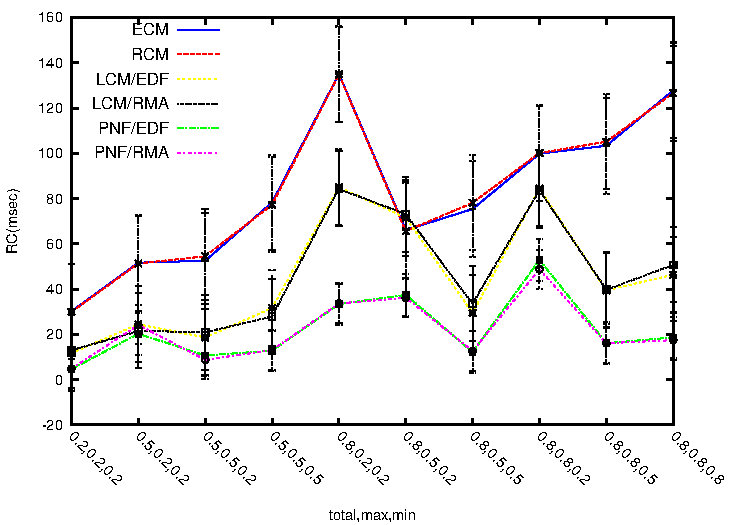
\includegraphics[scale=0.7]
{figures/Abr_dur_4t_100obj_40wr}
\label{fig:4t_ecm_rcm_lcm_pnf_100obj_40wr}
}
~
\subfigure[8 tasks]{
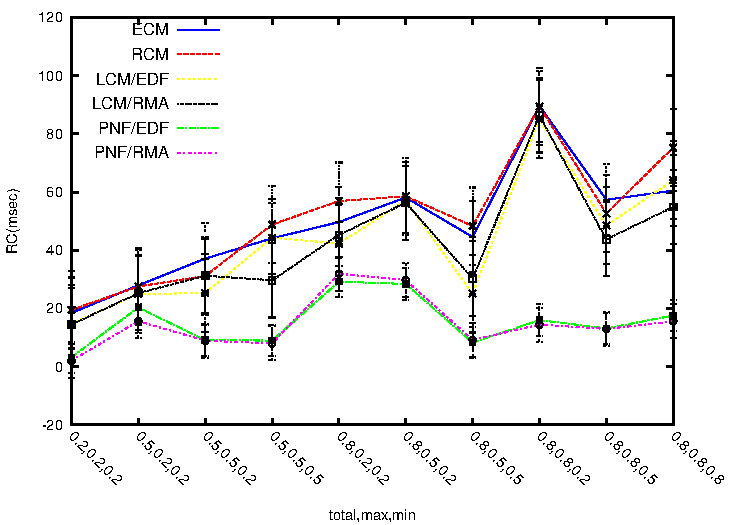
\includegraphics[scale=0.7]
{figures/Abr_dur_8t_180obj_40wr}
\label{fig:8t_ecm_rcm_lcm_pnf_180obj_40wr}
}
~
\subfigure[20 tasks]{
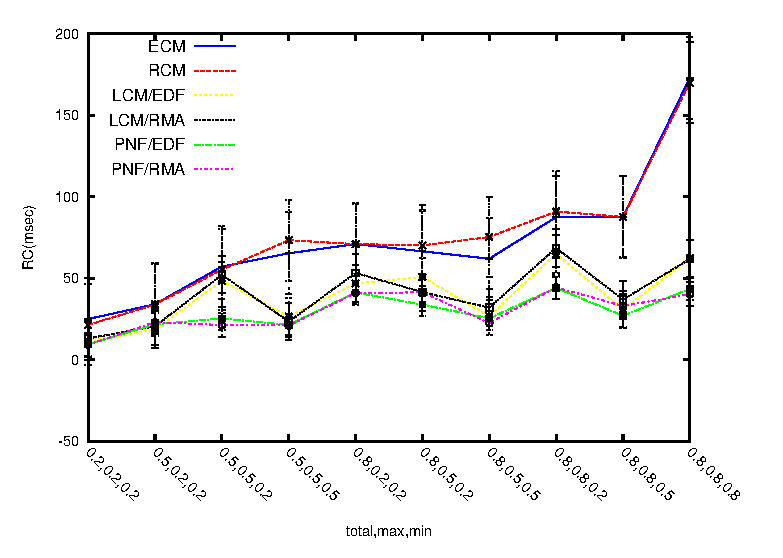
\includegraphics[scale=0.7]
{figures/Abr_dur_20t_420obj_40wr}
\label{fig:20t_ecm_rcm_lcm_pnf_420obj_40wr}
}
\caption{Average retry cost for 40 objects per transaction, 40\% write operations for different values of total, maximum and minimum atomic section length under different CMs}
\label{fig:cm_40obj_per_tx_40wr}
\end{figure}
%%%%%%%%%%%%%%%%%%%%%%%%%%%%%%%%%%%%%%%%%%%%%%%%%%%%%%
\begin{figure}
\centering

\subfigure[4 tasks]{
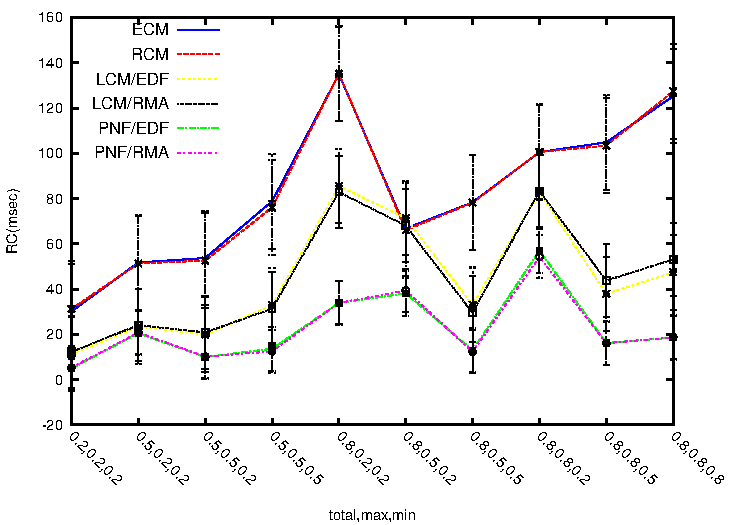
\includegraphics[scale=0.7]
{figures/Abr_dur_4t_100obj_80wr}
\label{fig:4t_ecm_rcm_lcm_pnf_100obj_80wr}
}
~
\subfigure[8 tasks]{
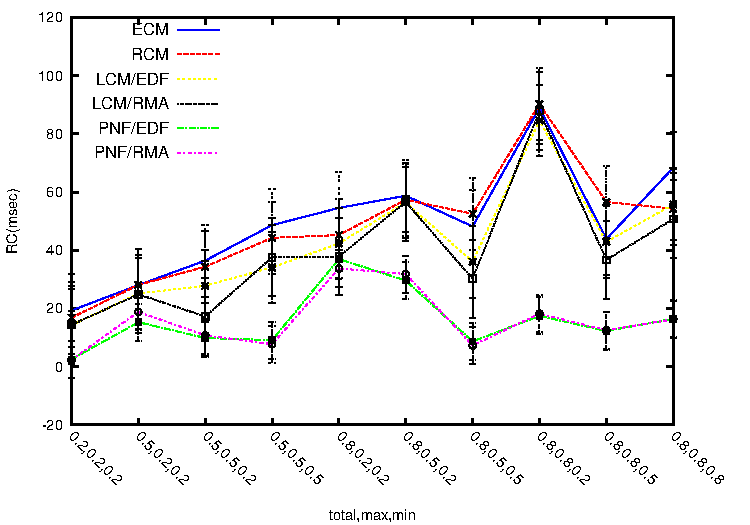
\includegraphics[scale=0.7]
{figures/Abr_dur_8t_180obj_80wr}
\label{fig:8t_ecm_rcm_lcm_pnf_180obj_80wr}
}
~
\subfigure[20 tasks]{
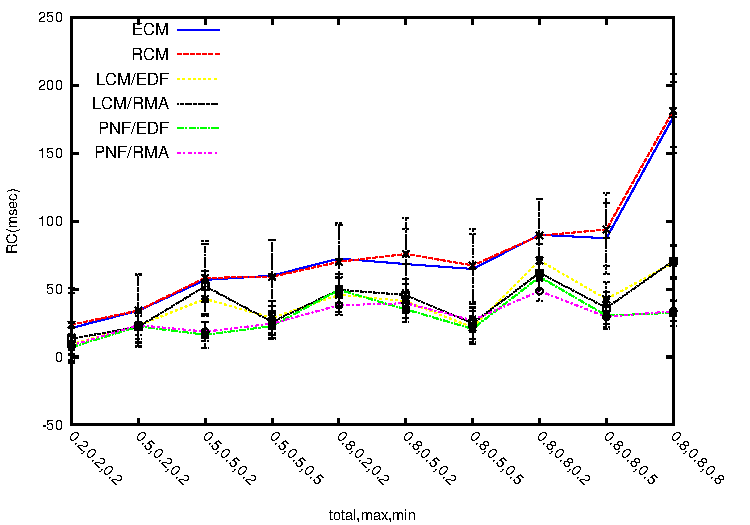
\includegraphics[scale=0.7]
{figures/Abr_dur_20t_420obj_80wr}
\label{fig:20t_ecm_rcm_lcm_pnf_420obj_80wr}
}
\caption{Average retry cost for 40 objects per transaction, 80\% write operations for different values of total, maximum and minimum atomic section length under different CMs}
\label{fig:cm_40obj_per_tx_80wr}
\end{figure}
%%%%%%%%%%%%%%%%%%%%%%%%%%%%%%%%%%%%%%%%%%%%%%%%%%%%%%
\begin{figure}
\centering

\subfigure[4 tasks]{
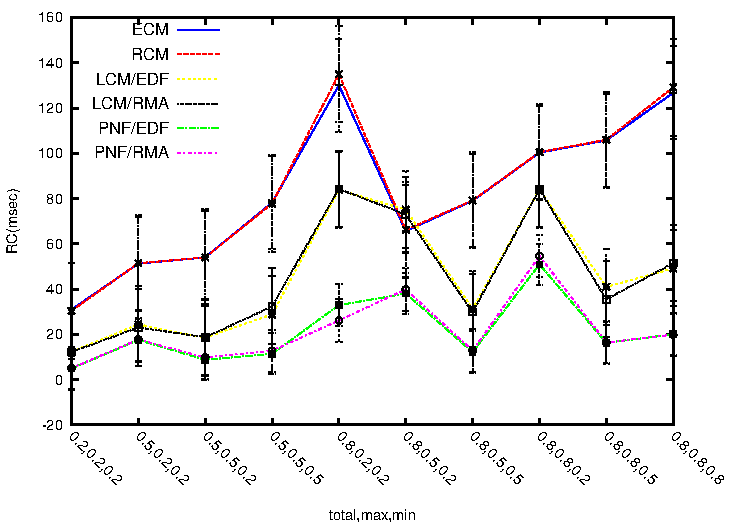
\includegraphics[scale=0.7]
{figures/Abr_dur_4t_100obj_100wr}
\label{fig:4t_ecm_rcm_lcm_pnf_100obj_100wr}
}
~
\subfigure[8 tasks]{
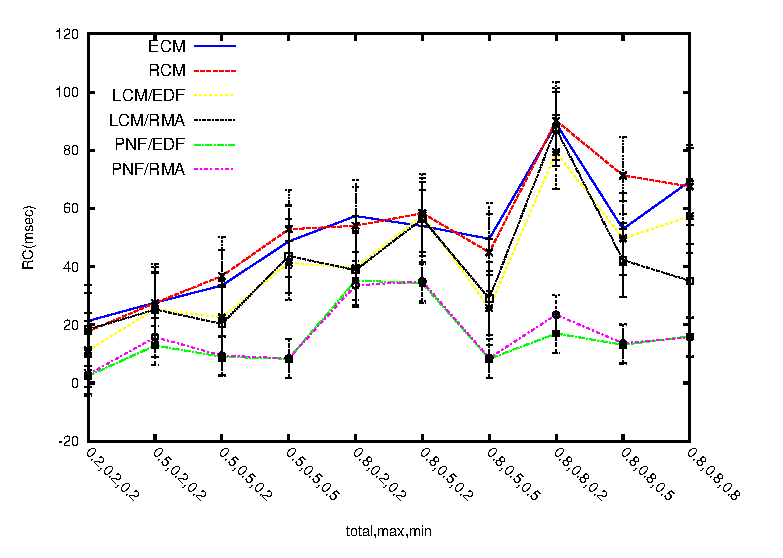
\includegraphics[scale=0.7]
{figures/Abr_dur_8t_180obj_100wr}
\label{fig:8t_ecm_rcm_lcm_pnf_180obj_100wr}
}
~
\subfigure[20 tasks]{
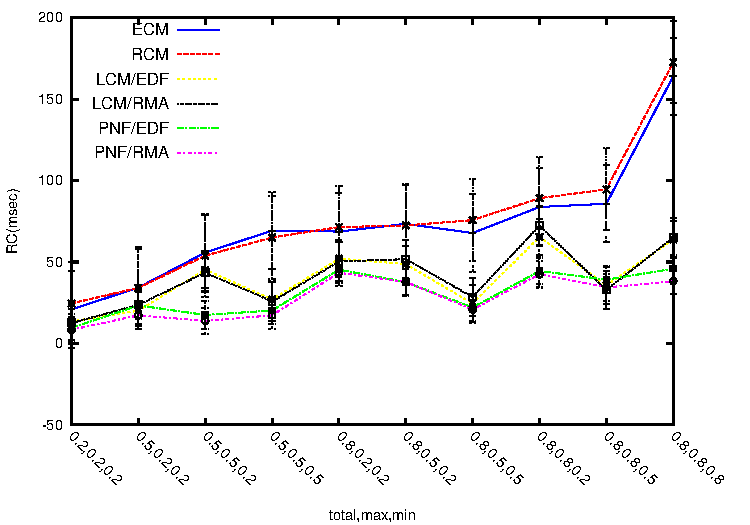
\includegraphics[scale=0.7]
{figures/Abr_dur_20t_420obj_100wr}
\label{fig:20t_ecm_rcm_lcm_pnf_420obj_100wr}
}
\caption{Average retry cost for 40 objects per transaction, 100\% write operations for different values of total, maximum and minimum atomic section length under different CMs}
\label{fig:cm_40obj_per_tx_100wr}
\end{figure}
%%%%%%%%%%%%%%%%%%%%%%%%%%%%%%%%%%%%%%%%%%%%%%%%%%%%%%

\chapter{\label{conclusions}Conclusions and Proposed Post Preliminary Exam Work}
\markright{Mohammed El-Shambakey \hfill Chapter~\ref{conclusions}. Conclusions and Proposed Post Preliminary Exam Work \hfill}

\section{Conclusions}

In this dissertation, we designed, analyzed, and experimentally evaluated four real-time CMs. Designing real-time CMs is straightforward. The simplest logic is to use the same rationale as that of the underlying real-time scheduler. This was shown in the design of ECM and RCM. ECM allows the transaction with the earliest absolute deadline (i.e., dynamic priority) to commit first. RCM allows the transaction with the smallest period (i.e., fixed priority) to commit first. We established upper bounds for retry costs and response times under ECM and RCM, and identified the conditions under which they have better schedulability than lock-free synchronization. 

Under both ECM and RCM, a task incurs $2.s_{max}$ retry cost for each of its atomic sections due to a conflict with another task's atomic section. Retries under RCM and lock-free synchronization are affected by a larger number of conflicting task instances than under ECM. While task retries under ECM and lock-free are affected by all other tasks, retries under RCM are affected only by higher priority tasks. 

STM and lock-free synchronization have similar parameters that affect their retry costs -- i.e., the number of conflicting jobs and how many times they access shared objects. The $s_{max}/r_{max}$ ratio determines whether STM is better or as good as lock-free. For ECM, this ratio cannot exceed 1, and it can be 1/2 for higher number of conflicting tasks. For RCM, for the common case, $s_{max}$ must be 1/2 of $r_{max}$, and in some cases, $s_{max}$ can be larger than $r_{max}$ by many orders of magnitude.

LCM, which can be used with both G-EDF and G-RMA, tries to compromise between priority of transactions (which is the priority of the underlying tasks), and the remaining execution time of the interfered transaction. As the remaining execution time of the interfered transaction decreases, it is not effective to abort the transaction when it can shortly commit. The parameters $\alpha$ and $\psi$ are used to determine whether or not to abort the interfered transaction. $\alpha$ ranges between 0 and 1. When $\alpha \rightarrow 0$, LCM defaults to FCFS. When $\alpha\rightarrow1$, G-EDF/LCM defaults to ECM, and G-RMA/LCM defaults to RCM. We also derived upper bounds on retry costs and response times under LCM, and compared the schedulability of LCM with ECM, RCM, and lock-free synchronization. Also, we identified the conditions under which LCM performs better than the other synchronization techniques. LCM reduces the retry cost  of each atomic section to $(1+\alpha_{max})s_{max}$, instead of $2.s_{max}$ as in ECM and RCM. In ECM and RCM, tasks do not retry due to lower priority tasks, whereas in LCM, they do so. In G-EDF/LCM, retry due to a lower priority job is encountered only from a task $\tau_{j}$'s last job instance during $\tau_{i}$'s period. This is not the case with G-RMA/LCM, because,  each higher priority task can be aborted and retried by any job instance of lower priority tasks. 

Schedulability of G-EDF/LCM and G-RMA/LCM is better or equal to ECM and RCM, respectively, by proper choices for $\alpha_{min}$ and $\alpha_{max}$. Schedulability of G-EDF/LCM and G-RMA/LCM is better or equal to lock-free synchronization as long as $s_{max}/r_{max}$ does not exceed 0.5. By proper choice of $\alpha$s, $s_{max}/r_{max}$ can be increased to 2 under G-EDF/LCM, and to larger values under G-RMA/LCM.

ECM, RCM, and LCM are affected by transitive retry. Transitive retry occurs when a transaction accesses multiple objects. It causes a transaction to abort and retry  due to another non-conflicting transaction. PNF avoids transitive retry, and and also optimizes the processor usage by reducing the priority of the aborted transaction. This way, other tasks can proceed if they do not conflict with other executing transactions. 

We upper bounded PNF's retry cost and response time. We also compared PNF's schedulability to other synchronization techniques. PNF has better schedulability than lock-free synchronization as long as $s_{max}$ does not exceed $r_{max}$. 

We also implemented the CMs and conducted experimental studies. Our experimental studies revealed that the CMs' have shorter retry costs than lock-free synchronization. In particular, PNF has shorter retry costs than others as long as transitive retry and contention exist. However, PNF's implementation is relatively complex. 



\section{Proposed Post Preliminary Exam Research}

We propose the following research directions:

\subsection{Supporting Nested Transactions} 

Transactions can be nested \textit{linearly}, where each transaction has at most one pending transaction~\cite{Moss2006186}. Nesting can also be done in \textit{parallel}, where transactions execute concurrently within the same parent~\cite{volos2009nepaltm}. Linear nesting can be \textit{1) flat:} If a child transaction aborts, then the parent transaction also aborts. If a child commits, no effect is taken until the parent commits. Modifications made by the child transaction are only visible to the parent until the parent commits, after which they are externally visible. 
%
\textit{2) Closed:} Similar to \textit{flat nesting}, except that if a child transaction conflicts, it is aborted and retried, without aborting the parent, potentially improving concurrency over flat nesting. 
%
\textit{3) Open:} If a child transaction commits, its modifications are immediately externally visible, releasing memory isolation  of objects used by the child, thereby potentially improving concurrency over closed nesting. However, if the parent conflicts after the child commits, then compensating actions are executed to undo the actions of the child, before retrying the parent and the child. 


We propose to develop real-time contention managers that allow these different nesting models and establish their retry and response time upper bounds. Additionally, we propose to formally compare their schedulability with nested critical sections under lock-based synchronization. Note that, nesting is not viable under lock-free synchronization.


The real-time CMs proposed so far can be directly extended for different types of nesting. On conflict, the CM should decide on which transaction must be  aborted. In case of flat nesting, the outer transaction should be aborted and restarted. In case of closed and open nesting, only the interfered transaction should be restarted. In flat nesting, it will be useful to delay a lower priority transaction when it interferes with a higher priority one. Thus, the lower priority transaction need not be restarted from the beginning. This can reduce retry costs, especially when the inner most transaction is the conflicting one.


ECM and RCM can use the same criteria to determine which transaction to abort or wait. LCM may need a redefinition of the $\alpha$ parameter. Each child transaction can have its own $\alpha$. So, for each depth of nesting, there is a corresponding $\alpha$. Alternatively, there can be only one $\alpha$ for the outer transaction. Inner transactions do not have their $\alpha$s. The first choice may be suitable for closed and open nesting, while the second choice seems more suitable for flat nesting. 


PNF can be used directly with all types of nesting. The only requirement is that each transaction checks for conflicts with itself, as well as its inner transactions. Executing transactions under PNF are non-preemptive. Thus, any nested transaction will not be aborted. This requirement for PNF simplifies implementation, but makes no use of the nesting structure (i.e., PNF deals with transactions as if they are not nested). The previous requirement for PNF can be alleviated by checking for conflicts of any inner transaction only when the inner transaction begins. So, when a transaction starts, it checks its own objects -- not inner transactions -- against objects of executing transactions. If no conflict is found, the transaction executes. Consequently, when an inner transaction starts, it can detect a conflict with already executing transactions. Thus, the inner transaction should wait until other conflicting executing transactions commit. This choice for the PNF implementation may add additional waiting time to inner transactions. Different choices thus impose different tradeoffs. 


Worst case response time analysis, similar to the design of CMs, needs modifications  to cope with nested transactions. The simplest method is to combine all accessed objects in all nested transactions into one group, and consider that this group is accessed by only one non-nested transaction. This simplifies calculations but loosens the upper bounds, especially with closed and open nesting. Since closed and open nesting only restarts the inner aborted transaction, it is of no use to include the length of the outermost parent in the response time calculations.


\subsection{Combining and Optimizing LCM and PNF} 

LCM is designed to reduce the retry cost of a transaction when it is interfered close to the end of its execution. In contrast, PNF is designed to avoid transitive retry when transactions access multiple objects. An interesting direction is to combine the two contention managers to obtain the benefits of both algorithms. 

An important problem in developing such a LCM/PNF combination is that LCM allows aborts of running transactions depending on the $\alpha$ value, whereas PNF does not permit aborts of any executing transaction. Thus, the first approach to combine LCM and PNF is by considering the transitive retry level. If the transitive retry level is high, then PNF could be used. Otherwise, LCM could be used. Another way to combine LCM and PNF is to change the $\alpha$ value with time. Thus, at some time point, $\alpha$ can equal $0$. This means that the current transaction cannot be aborted by any other transaction. This is similar to executing transactions in PNF. However, $\alpha$ should not be $0$ all the time. Thus, $\alpha$ should change with time.

For such a combined LCM/PNF contention manager, importantly, we must  understand what are its schedulability advantages over that of LCM and PNF individually, and how such a combined CM behaves in practice. 


The current implementation of PNF is centralized. In this implementation, PNF acts as a centralized contention manager that controls all transactions. Contention managers are usually decentralized, as described in Section~\ref{sec:contention manager}. Each transaction usually maintains its own contention manager; this reduces overhead and transaction blocking. Thus, one optimization direction is to develop a decentralized implementation of PNF, to reduce overhead and blocking. Moreover, the current implementation of PNF uses locks, which increases overhead. Another optimization direction is therefore to develop a lock-free PNF implementation.


Design optimizations of LCM and PNF may also be possible to reduce their retry costs and response times, by considering additional criteria for resolving transactional conflicts. 

Developing a LCM/PNF combination and optimizing PNF and LCM implementations and designs constitute  our second research direction. 

\subsection{Formal and Experimental Comparison with Real-Time Locking} 

Lock-free synchronization offers numerous advantages over locking protocols, but (coarse-grain) locking protocols have had significant traction in real-time systems due to their good programmability (even though their concurrency is low).  Example such real-time locking protocols include PCP and its variants~\cite{chen1990dynamic,6031129,Rajkumar:1991:SRS:532621,sha1990priority}, multicore PCP (MPCP)~\cite{lakshmanan2009coordinated,rajkumar2002real}, SRP~\cite{Buttazzo:2004:HRC:1027504, baker1991stack}, multicore SRP (MSRP)~\cite{gai2003comparison}, PIP~\cite{easwaran2009resource}, FMLP~\cite{key-4,brandenburg2008implementation,holman2006locking}, and OMLP~\cite{Baruah:2007:TMG:1338441.1338647}. FMLP has been established to be superior to other protocols~\cite{brandenburg2008comparison}. How does their schedulability compare with that of the proposed contention managers? How do they compare in practice? These questions constitute our third research direction. 

OMLP~\cite{key-3} is similar to FMLP, and is simpler in implementation. OMLP does not require changes in the underlying scheduler (i.e., G-EDF) as FMLP does. Under OMLP, each resource has a FIFO queue of length at most equals number of processors, $m$, and a priority queue. Requests for each resource are enqueued in the corresponding FIFO queue. If the FIFO queue is full, requests are added to the priority queue according to the requesting job's priority. The head of the FIFO queue is the resource holding task. Other queued requests are suspended until their turn arrives. Under suspension oblivious analysis for OMLP, each job has a maximum blocking time that is proportional to number of processors. In suspension oblivious, the suspension time is added to task execution, in contrast to suspension aware analysis. This is why
OMLP is asymptotically optimal under suspension oblivious analysis. We intend to implement OMLP in the ChronOS real-time OS. We also propose to analytically and experimentally compare OMLP against different CMs, including that for nested and non-nested transactions.



% If you are using BibTeX, uncomment the following:
% \thebibliography
%
% Otherwise, uncomment the following:
% \chapter*{Bibliography}

%%%%%%%%%%%%%%%%%%%%%%%%%%%%%%%%
\pagebreak 
\markright{Mohammed El-Shambakey \hfill Bibliography \hfill}
\bibliographystyle{plain}
\bibliography{/e/lectures/real-time/PhD-work/STM/writing/global_bibliography/global_bibliography}


% \appendix

% In LaTeX, each appendix is a "chapter"
% \chapter{Program Source}
%%%%%%%%%%%%%%%%%
%
% Include an EPS figure with this command:
%   \epsffile{filename}
%

%%%%%%%%%%%%%%%%
%
% Do tables like this:


\end{document}